% This sample file is dedicated to the public domain.
\documentclass[12pt]{myucthesis}

%\nofiles
% The above command prevents latex from writing its auxiliary
% files. This is useful if you want to manually tweak them before you
% generate your final PDF.


% Page layout. The fancyhdr package may complain about the need for a
% larger headheight, depending on how long chapter titles are; if left
% unspecified in the geometry setup, it defaults to 12pt. The
% "showframe" option causes the geometry package (version >= 5.0) to
% show a frame around the margins on every page, which is great for
% checking that you don't overflow anywhere.

%\usepackage[letterpaper,includehead,margin=1in,headheight=15pt,showframe]{geometry}
\usepackage[letterpaper,includehead,margin=1in,headheight=15pt]{geometry}
\usepackage{fancyhdr}
\pagestyle{fancyplain}
\lhead[\fancyplain{\thepage}{\thepage}]{\fancyplain{}{\scshape\rightmark}}
\rhead[\fancyplain{}{\scshape\leftmark}]{\fancyplain{\thepage}{\thepage}}
\chead{}
\cfoot{}
\lfoot{}
\rfoot{}


% Bibliography stuff:
\newcommand{\newblock}{\par} % need this for some natbib internal bug
\usepackage{natbib}
\citestyle{aa}
\bibliographystyle{yahapj}
\setlength{\bibsep}{0ex} % single-space entries
\def\bibpreamble{\addcontentsline{toc}{chapter}{Bibliography}} % get a good TOC entry


% Other setup:

\usepackage[T1]{fontenc} % see http://tinyurl.com/67zdxwf
\usepackage[colorlinks,urlcolor=blue,citecolor=blue,linkcolor=blue,pdfusetitle]{hyperref}
\usepackage{pdflscape} % allows landscape-oriented figures with PDF page rotation
\usepackage{aasmacros,amsmath,amssymb,graphicx}
\usepackage{mydeluxetable} % deluxetable customized to play well with ucthesis


\begin{document}
\ssp % single spacing
\hypersetup{pageanchor=false}
\title{Methods for the Detection of the Epoch of Reionization}
\author{Carina Cheng} % must match BearFacts!
\degreesemester{Spring}
\degreeyear{2019}
\degree{Doctor of Philosophy}
\numberofmembers{3}
\chair{Professor Aaron Parsons}
\othermembers{
Professor Stuart Bale \\
Professor Mariska Kriek 
}
\field{Astrophysics}
\campus{Berkeley}

\maketitle
\copyrightpage

\begin{abstract}
The Epoch of Reionization is one of the last unexplored eras of our Universe's history. Beginning about a billion years after the Big Bang, this epoch is characterized by the births of the first stars and galaxies, whose light subsequently altered the nature of the gas surrounding them. There are several experiments aiming to detect the phase transition of this gas as it changes from neutral hydrogen to ionized hydrogen. Such a detection would open a wealth of information about our early Universe, revealing details about the nature of the first luminous sources and the evolution of structure formation.

Interferometers such as the Precision Array for Probing the Epoch of Reionization (PAPER) and the Hydrogen Epoch of Reionization Array (HERA) seek to measure the 21\,cm signal from neutral hydrogen and map its evolution over spatial and temporal scales. A successful detection of reionization, however, is a difficult measurement. Though the 21\,cm signal is a powerful topological probe of the intergalactic medium, it is easily buried underneath bright foreground signals and instrumental systematics. A clean detection of reionization is ambitious and requires analysis methods that maximize data sensitivity and increase confidence in results.

The work presented in this thesis addresses many of the key challenges that face the current field of 21\,cm cosmology. This includes algorithms to locate contaminated data, methods to ensure accurate power spectrum measurements, and techniques for removing unwanted systematics while preserving the reionization signal. These developments serve as the foundation of the latest 21\,cm measurements from the PAPER-64 and PAPER-128 arrays, whose results lie at the forefront of the field. These methods are also fundamental to HERA and future experiments, as they provide a strong foundation for the continued exploration of our cosmic dawn.

\end{abstract}

\hypersetup{pageanchor=true}
\begin{frontmatter}

\begin{dedication}
\null\vfil
{\large
\begin{center}
\textit{to my parents}
\end{center}}
\null\vfil
\end{dedication}

\tableofcontents
\listoffigures % optional
\listoftables % optional

% If using code.sty, can also add:
%% \listofcodes
%% \addcontentsline{toc}{chapter}{List of Code Examples}

\begin{acknowledgements}
% Feel free to modify or remove this acknowledgment:
%This dissertation was typeset using the
%\href{https://github.com/pkgw/ucastrothesis}{\textsf{ucastrothesis}}
%\LaTeX\ template.
This thesis may be filled with new scientific methods, exciting astronomical insights, and technical jargon. But what it doesn't capture, is what I'm most proud of --- the life lessons I've learned about what it means to be a scientist, what it means to do good science, and how to learn and preservere despite challenges. For that, I must thank many people.


\end{acknowledgements}
\end{frontmatter}

\chapter{Introduction}
\label{c.intro}

\section{The Epoch of Reionization}

Our Universe has a complex, rich history, of which enormous progress has been made in the past few decades to unravel its story. Much has been learned about the very beginnings of the Universe, from the Big Bang's large explosion of energy to the relatively smooth and simple cosmic background radiation that was leftover. Additionally, observational feats have revealed the status of the present-day Universe and the intricate \textit{cosmic web}, or large scale structure, of galaxies today. 

The Epoch of Reionization (EoR) ties these two bookends together, occurring about a billion years after the Big Bang when the very first stars and galaxies formed. How did the tiny density fluctuations from the cosmic microwave background develop into the structure we see today? How did the first luminous structures form, and how did they evolve and influence the gas around them? Exploring the reionization era opens up a new chapter of our Universe's story - a chapter that promises to connect the dots between our past and present.

\subsection{Cosmic History}

As the Universe expanded and cooled after the Big Bang, electrons and protons eventually combined to form neutral hydrogen atoms. At the young age of $\sim$ $380,000$ years, the Universe's ordinary baryonic content was almost entirely neutral hydrogen, while most of its total matter was dark matter (\citealt{loeb_furlanetto_2013}). Then, for the next several hundred million years, the \textit{Dark Ages} proceeded, with concentrations of dark matter setting the foundations for the formation of the first luminous structures. More specifically, the tiny, primordial density fluctuations that were established at the release of the CMB grew with inflation and the expansion of the Universe. The densest regions then collapsed to form dark matter halos, inside of which hydrogen gas could cool, condense, and fragment into stars (\citealt{dodelson_cosmology}).

The first luminous structures are thought to have formed at an age of $\sim$ $200$ million years (z $\sim$ 20) and are predicted to have been massive stars with high luminosities and large ionizing powers (\citealt{loeb_furlanetto_2013}). The ionizing photons from the first stars carved out pockets of ionized hydrogen gas around the densest, most massive dark matter halos, and as the number of sources grew, an increased number of ionized bubbles emerged and overlapped. Eventually, the first generations of stars and galaxies succeeded in ionizing most all of the neutral hydrogen in the Universe, with reionization complete by about one billion years after the Big Bang (z $\sim$ 6) (\citealt{furlanetto_et_al2006}). 

\begin{figure}
	\centering
	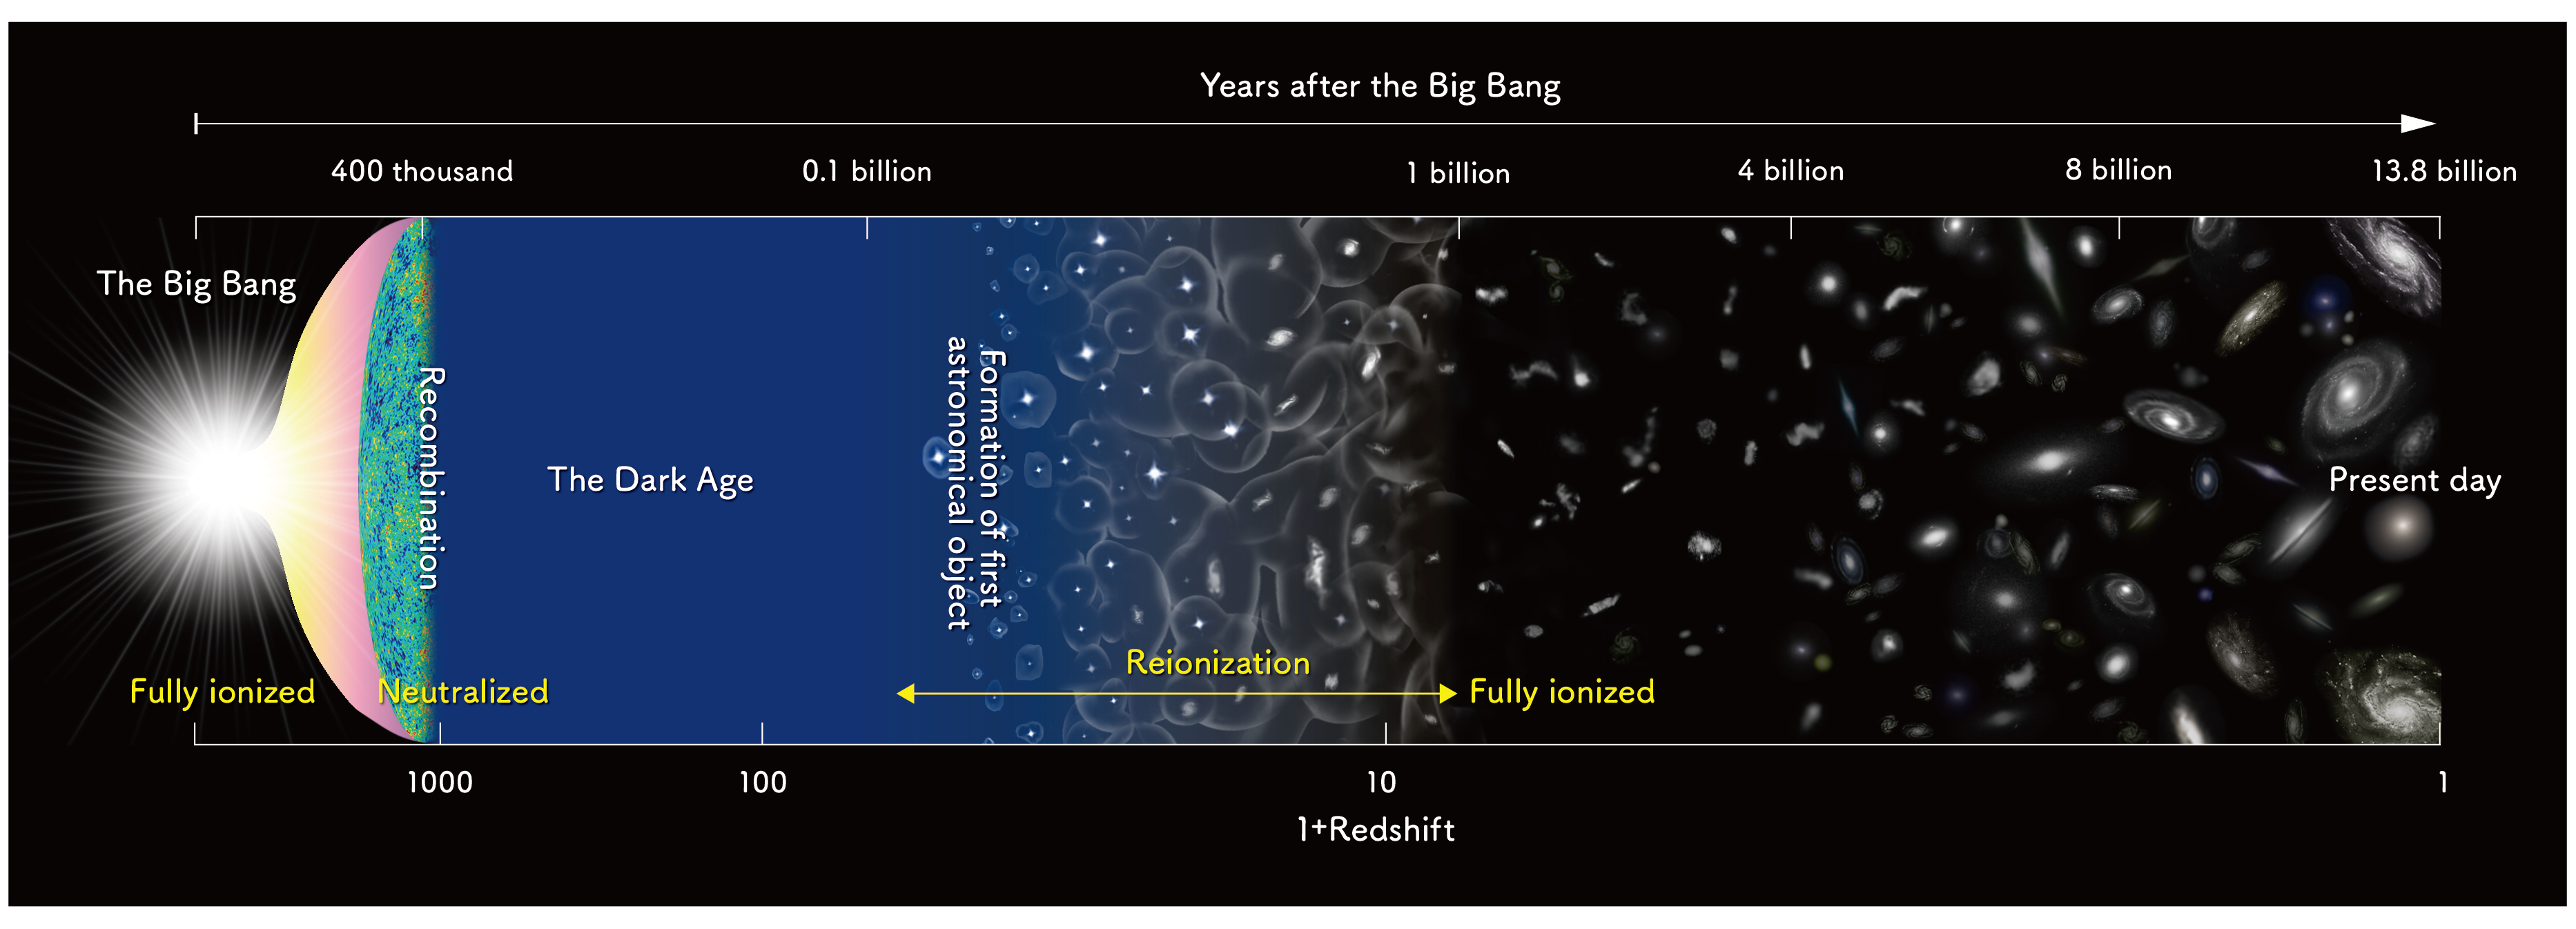
\includegraphics[width=\columnwidth]{plots/timeline_history.jpg}
	\caption{Timeline of the history of the Universe. The Epoch of Reionization marks the era when the first stars and galaxies formed and ionized the neutral hydrogen in the Universe. Image credit: NAOJ.}
	\label{fig:timeline_history}
\end{figure}

The exact timescale and details of the reionization process, which are shown within the context of the history of the Universe in Figure \ref{fig:timeline_history}, are current research questions in the field of cosmology. The physics of reionization depends on several factors, including the nature of the first stars (masses, luminosities, ionizing photons) and the surrounding gas (efficiency of the ionizing photons, feedback effects). Turning the argument around, deep investigations of the reionization era would lead to new understandings about the properties of the first stars and the intergalactic medium (IGM). There are several ways to approach the study of this epoch, with CMB measurements working to constrain the duration of reionization, galaxy measurements unveiling the end of reionization, and direct hydrogen measurements attempting to map out the changing nature of the gas over time. All of these probes serve to illuminate this watershed era between a Universe dominated by darkness and a Universe defined by light.

\subsection{CMB and Galaxy Measurements}

There are several observational probes of the reionization epoch, and we highlight two broad categories in this section. The first is the study of CMB anisotropies, which carry with them an imprint of the early Universe from the time of its release. But that's not the only imprint it has - CMB photons can scatter off of free electrons after reionization, and these scatterings leave behind polarization and temperature imprints (\citealt{haiman_knox_1999}). For example, the amplitude of the CMB is sensitive to scatterings, as an increased number of scatterings is akin to mixing different parts of the CMB together as photons are scattered in all directions. In other words, this scattering washes out anisotropies in the CMB and lowers its overall amplitude. 

A useful parameter to quantify the amount of electron scattering that occurs is the optical depth, $\tau_{es}$, defined as:

\begin{equation}
\tau_{es} = \int n_{e}\sigma_{T} dl,
\end{equation}
where $n_{e}$ is the number density of free electrons, $\sigma_{T}$ is the Thompson cross-section, and the integral is taken over a proper length $dl$. Once reionization begins, the number of free electrons increases, contributing to increasingly higher values of $\tau_{es}$. Hence, an earlier start for reionization would yield higher optical depths than a late reionization scenario. 

Observations of the CMB by WMAP and Planck have placed constraints on the optical depth parameter (\citealt{hinshaw_et_al2013}; \citealt{planck2016}), with the more recent Planck result suggesting a value of $\tau_{es} \sim 0.07$. This value suggests that reionization ends at a redshift of $z \sim 6$, with instantaneous reionization (``mean" reionization) at $z \sim 8.8$ (\citealt{planck2016}).

Currently, the results from CMB measurements are in agreement with a second powerful probe of EoR --- broadly speaking, that of galaxy observations. This probe comes in many flavors. For example, the spectra of distant quasars at high redshifts can illuminate the end of reionization. Quasars, being extraordinarily bright and energetic objects, are detectable at very far distances and their spectra reveal the amount of absorption their light has undergone due to neutral hydrogen. While nearby quasar spectra exhibit sharp absorption lines, distant ones show the Gunn-Peterson trough, implying that the quasar light was entirely suppressed by hydrogen absorption (i.e., neutral hydrogen existed). Studying the absorption features of quasars at different redshifts implies that reionization has indeed ended by $z \sim 6$ (\citealt{becker_et_al2001}). 

In addition to quasar observations, high-redshift galaxy observations can also reveal important characteristics about the state of the IGM. Namely, distant star-forming galaxies can be detected using a variety of techniques, such as narrow-band imaging to find Lyman-$\alpha$ emitters (radiation that is produced by recombination near young stars) or broad-band observations to find Lyman-break galaxies (spectral breaks associated with absorption by neutral hydrogen). High-redshift galaxy observations can then be used to construct luminosity functions (number of stars per luminosity interval) and star formation histories, which in turn impact the evolution of the IGM. 

More specifically, if star-forming galaxies dominated the reionization process, then the ionization rate can be related to the following star-formation parameters:

\begin{equation}
\dot{n}_{\rm ion} = f_{\rm esc}\xi_{\rm ion}\rho_{\rm SFR},
\end{equation}
where $\dot{n}_{\rm ion}$ is the cosmic ionization rate, $f_{\rm esc}$ is the escape fraction of photons into the IGM, $\xi_{\rm ion}$ is the rate of production of ionizing photons for a stellar population, and $\rho_{\rm SFR}$ is the star formation rate density. All three parameters influence the rate at which the IGM is ionized, and the star formation rate density is able to be constructed from galaxy luminosity functions. For example, \citet{robertson_et_al2015} used data from the Hubble Space Telescope to construct a star formation rate history out to high redshifts, backing out an optical depth parameter that is consistent with that of Planck. 

While galaxy measurements can be used to constrain the EoR, they are ultimately doing so by unveiling the properties of old, distant stars and galaxies. A similar, new technique that also aims to reconstruct the histories of the first luminous structures is observing nearby, metal-poor Local Group galaxies. Called ``galactic archaeology," observations of nearby star-forming ancestors can be used to constrain the faint-end slope of the luminosity function. Determining the shape of this function has important implications on the number of galaxies needed to drive reionization and the types of sources dominating this epoch (\citealt{weisz2017}). Additionally, studies of nearby metal-poor stars and galaxies can provide insight into the contents of the first generation of stars and the dynamics of high-redshift star formation, as observations of ultrafaint dwarf galaxies around the Milky Way suggest they are relatively clean tracers of the first generations of stars (\citealt{loeb_furlanetto_2013}).

Galaxy observations for reionization studies have been primarily driven by observations taken by the Hubble Space Telescope. In the coming years, the James Webb Space Telescope (JWST), a 6.5\,m infrared space telescope, will be optimally primed for the detection of faint galaxies, including galaxies whose roots extend as far back as the cosmic dawn and who may exhibit signatures of first generation Population III stars. In addition to JWST, several large infrared ground telescopes are also underway, including the European Extremely Large Telescope (EELT), the Giant Magellan Telescope (GMT), and the Thirty Meter Telescope (TMT). 

Although both CMB measurements and galaxy observations have much to look forward to, they currently each have their limitations. For example, CMB measurements can only reveal the integrated quantity of $\tau_{es}$, therefore unable to provide insight into the evolution of reionization as it progresses over time. Similarly, galaxy observations are currently limited by sensitivity, able to hover only around the tail end of the reionization era. A different, but complimentary, probe is needed to unlock the entire window into the EoR.

\subsection{Measurements of HI}

A direct measurement of neutral hydrogen gas over time would provide a fundamental way to track the IGM over the reionization process. Such a probe, which is made possible by the spin-flip transition of hydrogen, is a powerful technique that allows the tracing of gas over time, and it is this technique that serves as the basis for the remainder of this thesis (\citealt{furlanetto_et_al2006}; \citealt{barkana_and_loeb2008}; \citealt{morales_and_wyithe2010}; \citealt{pritchard_and_loeb2010}; \citealt{pritchard_loeb2012}). 

The spin-flip transition of neutral hydrogen occurs when a hydrogen atom changes energy state between two hyperfine levels. Namely, if a hydrogen atom moves from an aligned energy state (the proton and electron have parallel spins) to an anti-aligned state (the proton and electron have antiparallel spins), the energy difference is released in the form of a photon with a wavelength of $21$\,cm. 

Because this transition has a well-defined wavelength, the signal can be directly mapped to a distance, or redshift, by measuring its wavelength upon detection. For example, a $21$\,cm photon that was initially emitted at a redshift of $z = 6$ would have expanded by a factor of ($1+z$) due to the expansion of the Universe and be $1.5$\,m long when it arrives at our telescopes. Hence, observing longer wavelengths of the hydrogen signal means that it has traveled for a greater distance (and has stretched out more) and thus comes from farther away at a higher redshift. This means that the $21$\,cm signal is a powerful tracer of neutral hydrogen at any distance (i.e., as a function of time), as long as it exists. This technique is especially compelling because it allows the direct exploration of the EoR as reionization occurs, whereas CMB measurements and galaxy measurements surround this era from the beginning and end only, respectively (Figure \ref{fig:timeline_circle}).

\begin{figure}
	\centering
	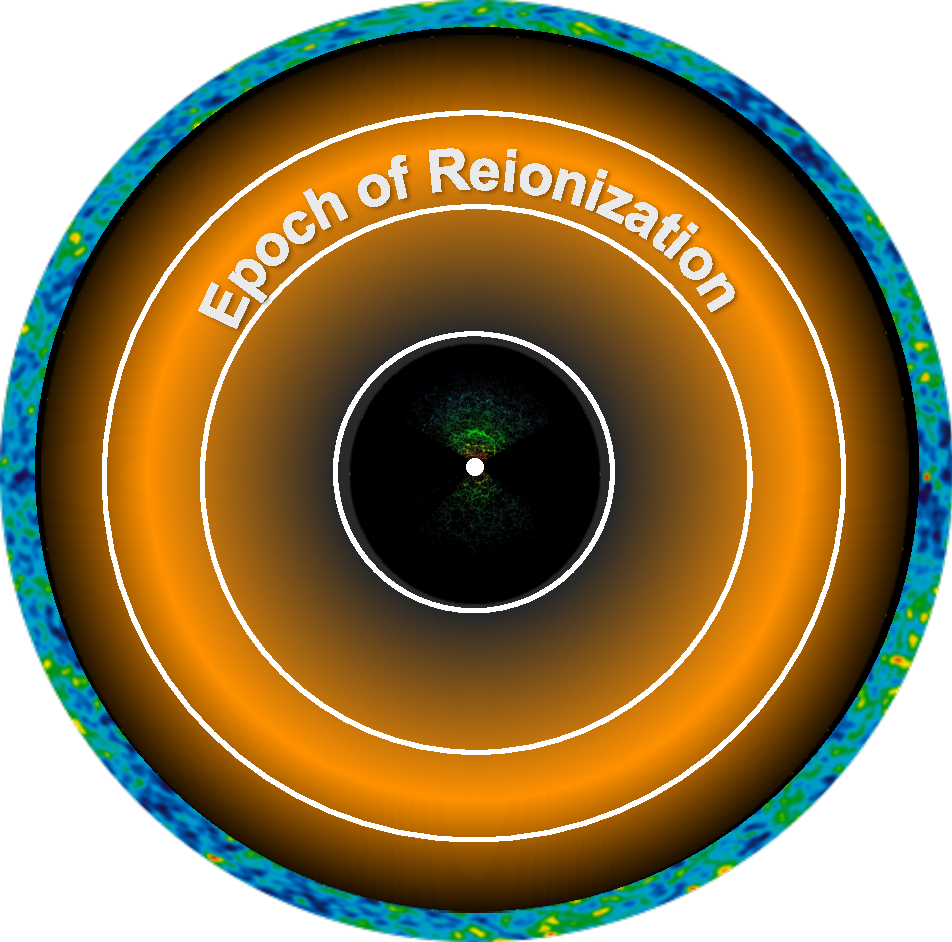
\includegraphics[width=0.5\textwidth]{plots/timeline_circle.pdf}
	\caption{A cartoon diagram of the observable Universe, centered on us. Close-by, galaxy observations have mapped out cosmic web structure in our nearby Universe (image credit: SDSS). Far-away, the cosmic microwave background is observed at a redshift of $z \sim 1100$ (image credit: WMAP). The Epoch of Reionization represents a largely unexplored era between the two, and can be probed by measuring red-shifted $21$\,cm radiation from neutral hydrogen.}
	\label{fig:timeline_circle}
\end{figure}

\begin{figure}
	\centering
	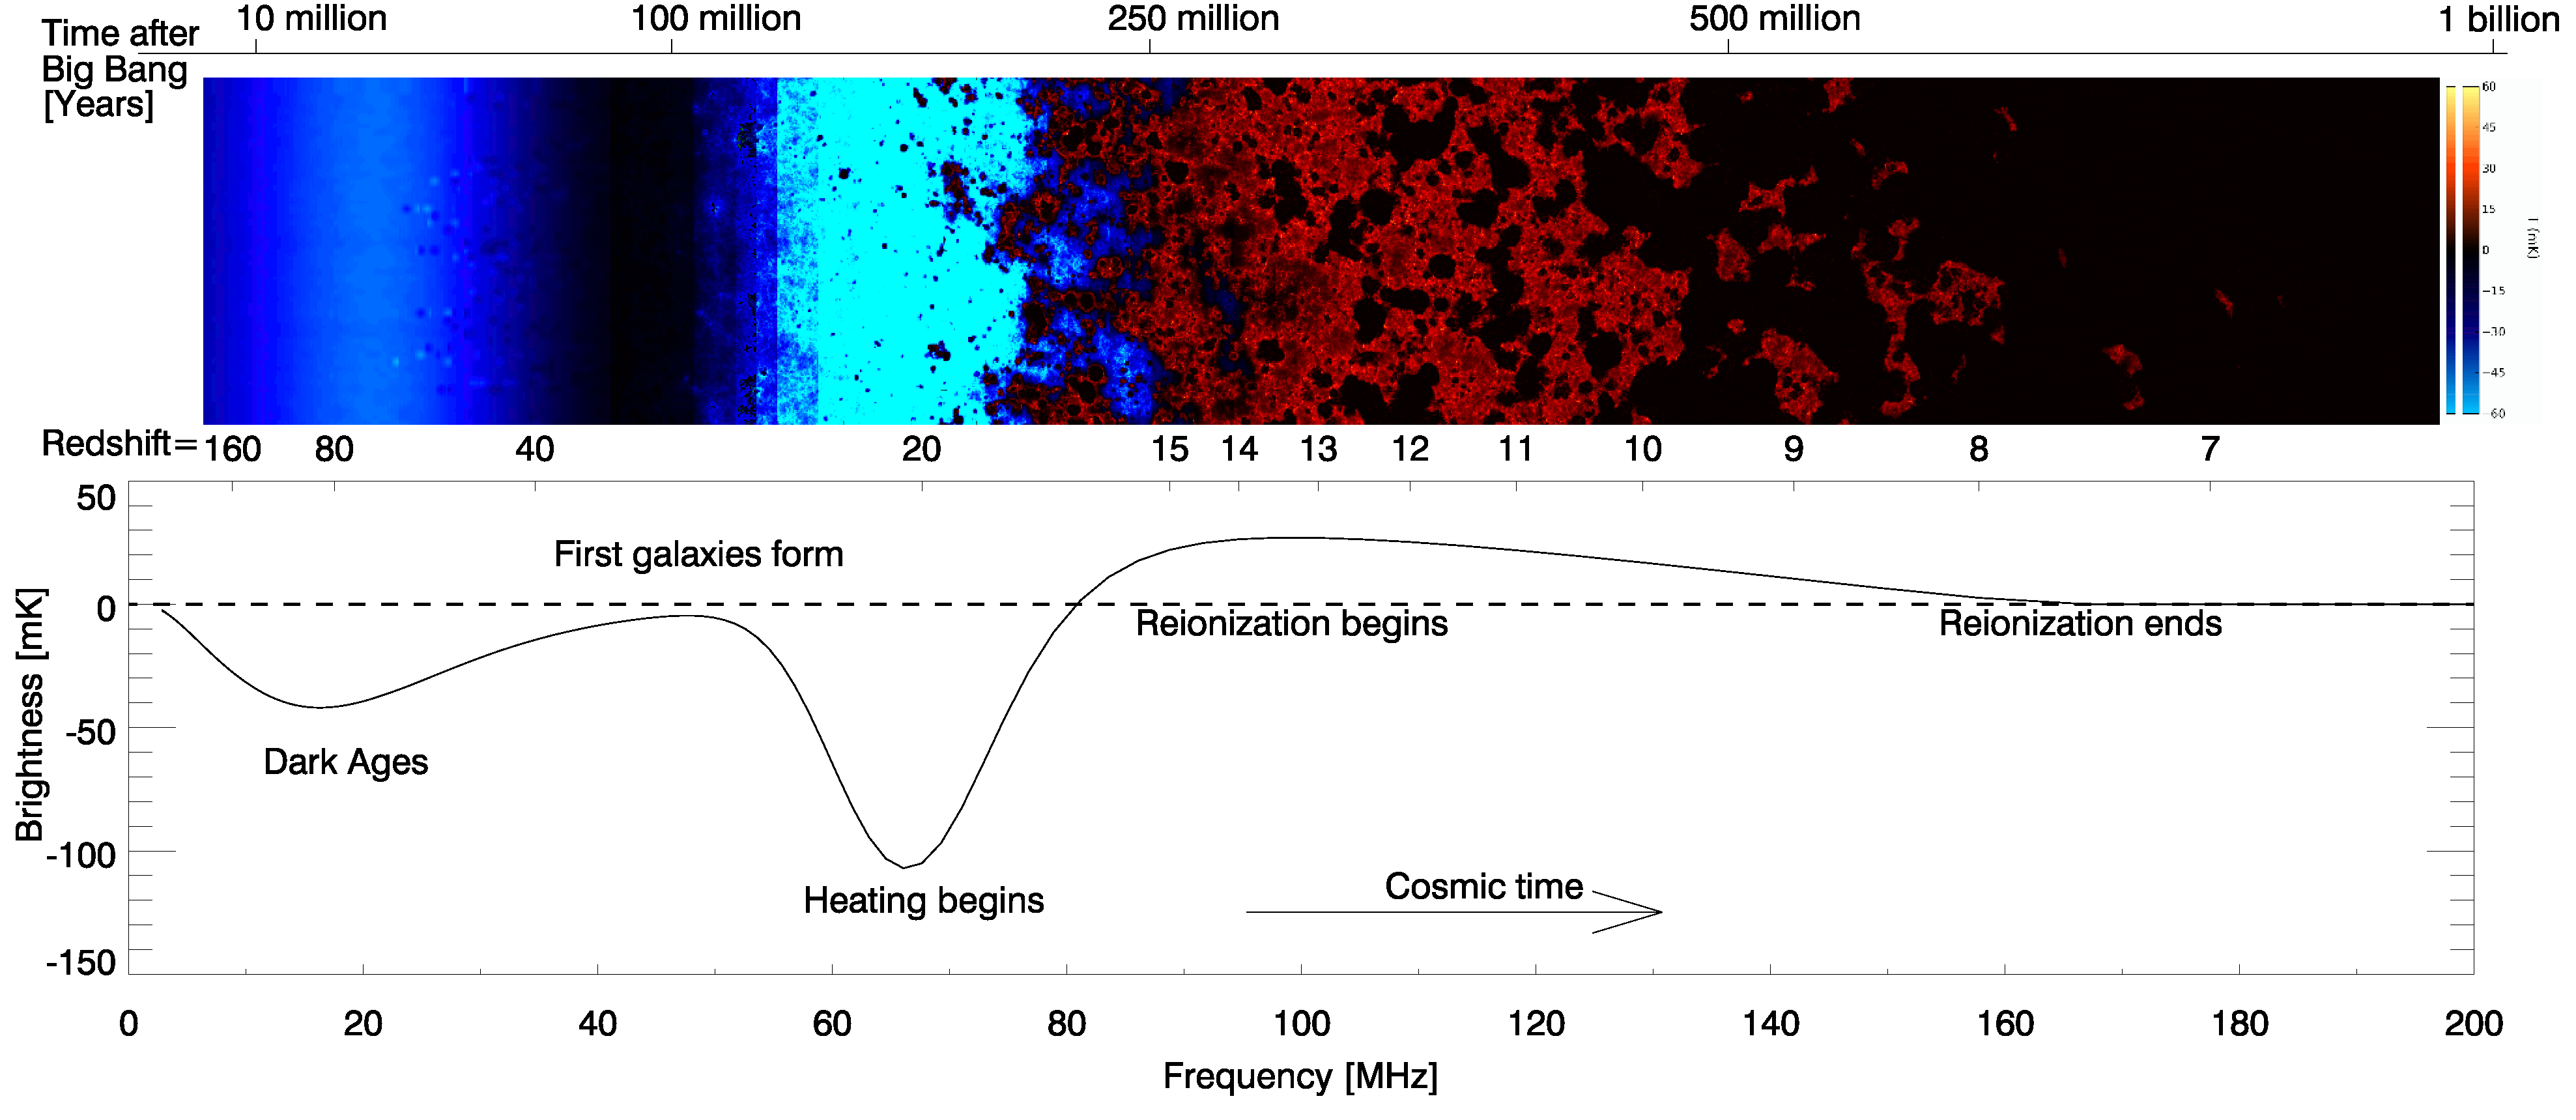
\includegraphics[width=\columnwidth]{plots/timeline_global.pdf}
	\caption{The evolution of the global $21$\,cm signal, starting with the Dark Ages, through galaxy formation and reionization (image credit: \citet{pritchard_loeb2012}). The work in this thesis mainly focuses on a redshift range of $6 < z < 12$ when reionization is expected to progress and complete.}
	\label{fig:timeline_global}
\end{figure}

In practice, the $21$\,cm signal is encapsulated by the quantity $T_{\rm spin}$ (spin temperature), which measures the relative number of hydrogen atoms in the excited (aligned) versus ground (anti-aligned) spin-flip state. A high spin temperature means that the hydrogen gas is more likely to emit $21$\,cm photons, whereas a low $T_{\rm spin}$ implies that the gas is more likely to absorb $21$\,cm photons. 

The spin temperature is always measured with respect to the temperature of the CMB ($T_{\rm CMB}$), which serves as a backlight for our measurement. During different stages of our cosmic history, $T_{\rm CMB}$ and $T_{\rm spin}$ take turns in the spotlight, with the \textit{differential brightness temperature} $\delta T_{b}$ describing their evolution:

\begin{equation}
\label{eq:Tb}
\delta T_{b} \propto (1+\delta_{b})x_{HI}\Big(1-\frac{T_{\rm CMB}}{T_{\rm spin}}\Big).
\end{equation}
Equation \eqref{eq:Tb} captures the EoR signal that $21$\,cm experiments seek to measure, where $\delta_{b}$ is the fractional over-density of matter and $x_{HI}$ is the fraction of neutral hydrogen ($1$ if all neutral, $0$ if all ionized). The differential brightness temperature can be measured in multiple ways --- in Chapter \ref{sec:interferometry} we explain how interferometry (multiple telescopes) can be used to measure the correlations of $\delta T_{b}$ on various spatial scales on the sky. Here we describe the evolution of the sky-averaged $\delta T_{b}$, called the \textit{global signal}, in order to summarize how it is expected to behave during our cosmic dawn and through reionization.

A theoretical prediction for the evolution of $\delta T_{b}$ is shown in Figure \ref{fig:timeline_global}. At the very far left, a cool, neutral IGM remains after recombination and the release of the CMB. Residual electrons collide off of both CMB photons and the hydrogen gas, driving couplings between $T_{\rm gas}$ and $T_{\rm CMB}$, and $T_{\rm gas}$ and $T_{\rm spin}$, respectively. Hence, we expect to see no signal ($\delta T_{b} = 0$) at this time.

During the Dark Ages, collisions still couple $T_{\rm gas}$ and $T_{\rm spin}$, but Compton scattering becomes rarer as the CMB dilutes with the expansion of the Universe. While the CMB dilutes as $T_{\rm CMB} \propto 1/a$, where $a$ is the scale factor, the gas now follows an adiabatic expansion ($T_{\rm gas} \propto 1/a^{2}$). Thus, the gas cools quicker than the CMB, and since it is still coupled to the spin temperature, $T_{\rm spin} < T_{\rm CMB}$ and the signal is expected to be seen in absorption. By the time the first galaxies begin forming, however, the gas is expected to be so dilute that it is no longer coupled to the spin temperature. The spin temperature therefore couples once again to the CMB, and no signal is produced.

As the first stars in the first galaxies begin emitting Lyman-$\alpha$ photons, they are resonantly scattered off of hydrogen via the Wouthuysen-Field effect (the absorption and emission of Lyman-$\alpha$ photons redistributes the spin-flip states), coupling $T_{\rm spin}$ and $T_{\rm gas}$ (\citealt{pritchard_and_loeb2010}). The gas, still cool from adiabatic expansion, implies that $T_{\rm spin} < T_{\rm CMB}$ and the signal is seen in absorption. Eventually, due to their long mean free paths, x-rays from the first sources are thought to be the primary drivers behind heating of the cooled, low-density gas (\citealt{furlanetto_et_al2006}). This drives both the gas and spin temperatures above that of the CMB, where the signal is expected to be seen in emission for the first time. 

Finally, even though the timing and details of reionization are unknown, UV photons from the first luminous structures are believed to eventually ionize all the neutral hydrogen, leaving no signal to be detected by a redshift of $z \sim 6$. 

The shape of the global signal holds important science implications about our early Universe. For example, the timing of the heating trough reveals the types of sources responsible for heating (i.e., late heating implies harder x-ray spectras for x-ray binaries, as shown in \citet{fialkov_et_al2014}). It also contains information regarding the sizes of the dark matter halos hosting those first sources and the cooling mechanisms responsible for star formation (\citealt{fialkov_et_al2014b}). The shape of the absorption feature is also dependent on a number of factors, such as x-ray and Lyman-$\alpha$ emissivities, which in turn are dependent on the nature of the first sources and properties of star formation. For high Lyman-$\alpha$ production rates, a deep trough would be present due to strong couplings between $T_{\rm spin}$ and $T_{\rm gas}$ as the gas cools. An even more pronounced absorption signature, such as the first tentative detection from the Experiment to Detect the Global Epoch of Reionization Signature (EDGES), requires additional physical explanations beyond known physics and commonly accepted scenarios (\citealt{bowman_et_al2018}). 

If the global signal's primary absorption feature unlocks clues about the first sources, the reionization peak and its subsequent decay hold the key for understanding the evolution of the neutral fraction $x_{HI}$. Namely, a direct measurement of $\delta T_{b}$ during this time would shed light about the duration and rate of the reionization process, which in turn can be translated into an evolution for $x_{HI}$. A long reionization duration, for example, would yield a slowly varying neutral fraction evolution, while a more instantaneous reionization would produce a sharp drop-off feature (\citealt{pritchard_and_loeb2010}). One thing is for certain though --- as the field continues to investigate our cosmic dawn through HI measurements (both the global signal and statistical fluctuations), we can expect to learn much about the constituents that make up the Universe and their complex interactions during this era.

\subsection{This Thesis}

Although $21$\,cm observations promises an uninterrupted window into the EoR, from which we can learn much about galaxy formation and the properties of the IGM, there are many challenges facing this field of cosmology. In general, the $21$\,cm signal is extremely faint, with bright foregrounds (mostly synchrotron radiation from our own Galaxy) and radio interference easily overshadowing the target signal. As a consequence, instruments need to be extremely well-understood, precisely calibrated, and sensitive enough for a successful detection. In addition, analysis techniques must be innovative and rigorously construed so as to be able to extract clean and accurate measurements.

In this thesis, I present work associated with data from radio interferometers seeking to measure $21$\,cm fluctuations during the EoR. While a confirmed detection by an interferometer remains elusive at this time, this work serves as a huge leap forward in working with large datasets and extracting measurements of the cosmological signal with confidence. The rest of this thesis thus focuses on the characterization of data from large telescope arrays in order to place accurate, stringent limits on the EoR signal. This field is still young, and the work in this thesis serves as a foundation of what promises to be an eye-opening adventure to-come.

\section{Interferometry}
\label{sec:interferometry}

Multiple radio telescopes (i.e., an interferometer) can be used in combination to probe $21$\,cm fluctuations. Rather than a single element, or aperture, many antennas can be used to increase the effective aperture size of the telescope.

As a simplistic example, two antennas may observe the same sky but each receives the sky signal at slightly different times, with a time delay determined by the antenna spacing, or baseline orientation and length, with respect to the sky. The two voltage streams from the antennas can then be correlated to form an output response with an amplitude dependent on the sky's intensity and a phase dependent on the time delay between the two elements and the frequency of the light. The power received by this baseline, as we will see, represents one sample in the large ``synthesized" aperture of the interferometer. Knowledge of the entire sky can be built up by having a large number of antennas and many different types, and copies, of baselines.

\subsection{The Visibility Equation}

The output measurement from correlating signals between two antennas is called a \textit{visibility}. The visibility can be written as:

\begin{equation}
\label{eq:vis}
V_{ij}(\nu) = S(\nu) e^{-2\pi i\frac{\vec{b}_{ij}\cdot \hat{s}}{\lambda}},
\end{equation}
where $i$ and $j$ represent a pair of antennas, $S(\nu)$ is the sky flux density, $\vec{b}_{ij}$ is the baseline vector, $\hat{s}$ is a unit-vector in the direction of a source in the sky, and $\lambda$ is the wavelength of the signal. The fractional term in the exponential reflects the changing number of wavelengths between the two antennas as a signal goes in and out of phase as the source passes overhead. The entire exponential term represents the phase of the visibility, which can also be described as the fringe pattern, or diffraction, or interference pattern, between two antenna elements. 

Equation \eqref{eq:vis} represents a visibility measurement for one direction on the sky. In practice, we compute the integrated visibility over the entire angular sky $d\Omega$:

\begin{equation}
V_{ij}(\nu,\Omega) = \int A(\nu,\Omega)I(\nu,\Omega) e^{-2\pi i\frac{\vec{b}_{ij}\cdot \hat{s}(\Omega)}{\lambda}}d\Omega,
\end{equation}
where the amplitude component has been broken up into a primary beam component $A(\nu,\Omega)$ and sky intensity component $I(\nu,\Omega)$. The primary beam describes the power pattern of an antenna element and determines its field of view. The total power received by an antenna can therefore be thought of as a combination of the intensity distribution on the sky and how receptive the antenna is, or more specifically, the convolution between the two terms (\citealt{thompson_et_al2001}).

The visibility equation can be re-interpreted as the 2-dimensional Fourier-transform of the sky, or a sample of the \textit{uv}-plane, where $u$ and $v$ are sine-waves in a 2D image. In other words, every baseline measures a different Fourier-mode of the sky. To form an image, the Fourier-transform of a visibility would produce a \textit{dirty image} of the sky, from which the true sky can be reconstructed by de-convolving out information from the antenna beam. In this thesis, however, we focus on the 3D Fourier-transform of the sky, or the power spectrum (Chapter \ref{sec:PSoverview}), instead of making images. Hence, we work directly with visibilities as a starting point, which has already taken two Fourier-transforms for us. 

\subsection{The $21$\,cm Power Spectrum}
\label{sec:PSoverview}

In this thesis, we focus on cross-correlations, or power spectral measurements, of visibilities. Recalling that we seek to measure the differential brightness temperature on various spatial scales of the sky, we can form the quantity:

\begin{equation}
\label{eq:PSdef}
\langle \delta \tilde{T}_{b}(\vec{k})^{\ast} \delta \tilde{T}_{b}(\vec{k})\rangle = (2\pi)^{3} \delta^{D}(\vec{k}-\vec{k}')P_{21}(\vec{k}) ,
\end{equation}
where $\delta \tilde{T}_{b}(\vec{k})$ is the Fourier-transform of the differential sky brightness as a function of cosmological wavenumber $\vec{k}$ (i.e., our visibility measurement, up to scaling factors), $\delta^{D}$ is the Dirac-delta function, and $P_{21}$ is the $21$\,cm power spectrum quantity we are interested in eventually forming.

Simply speaking, because our visibility measurements have already taken two spatial Fourier-transforms out of the three needed for a 3D power spectrum, we need only to take one last Fourier-transform (along frequency), and then multiply and average the visibilities together for a given baseline in order to compute a power spectral measurement. Having repeated baseline copies then increases the sensitivity to a given Fourier-mode on the sky, while having different types of baselines makes it possible to measure multiple Fourier-modes and build up an image of the sky. Since the EoR signal is expected to be present everywhere on the sky, in this work we focus on the former technique in order to maximize our sensitivity to the cosmological signal.

We note that the wavenumber $\vec{k}$ can be broken up into a perpendicular component $\vec{k}_{\perp}$ and a parallel component $k_{\parallel}$, where $\vec{k}_{\perp}$ is proportional to the (x,y) spatial coordinates on the sky and $k_{\parallel}$ is proportional to the line-of-sight direction on the sky (i.e., frequency). Every unique baseline probes a single $\vec{k}_{\perp}$, and it's worth noting that, because we focus on redundant baselines in the analysis to follow, most of our power spectrum sensitivity comes from the frequency-direction. Accounting for cosmological distance, a 1D wavenumber has units of Mpc$^{-1}$, so that the 3D power spectrum has units of mK$^{2}\cdot$Mpc$^{3}$. Visibility measurements typically have units of Janskys.

Just as the shape of the global signal provides insight about the early Universe, the shape of the cross-power spectrum, as defined by Equation \eqref{eq:PSdef}, also delivers a wealth of information. Figure \ref{fig:PS_evolution} shows the $21$\,cm ``dimensionless" power spectrum $\Delta^{2}(k)$ (units of mK), defined as:

\begin{equation}
\Delta^{2}(k) = \frac{k^{3}}{2\pi^{2}}P_{21}(k),
\end{equation}
as a function of the magnitude of $k$. This figure shows the expected evolution of the power spectrum, where the overall signal moves to small scales (large $k$) as more hydrogen becomes ionized (the large regions of neutral hydrogen turn into smaller and smaller pockets). This effect can be seen by both the steepening of the spectrum as the neutral fraction decreases, and the time-evolution of the spectrum at a specific (large) $k$.

The $21$\,cm power spectrum therefore encodes important information about the spatial and temporal evolution of reionization, and the shape of the spectrum can be directly mapped to sizes of the ionized bubbles as they grow. Additionally, the power spectrum, which is a function of the differential brightness temperature, can be used to constrain both $T_{\rm spin}$ (and $T_{\rm gas}$, since they're coupled during this era) and $x_{HI}$ via Equation \eqref{eq:Tb}. It is thus a powerful tool for unlocking the properties of the IGM.

\begin{figure}
    \centering
    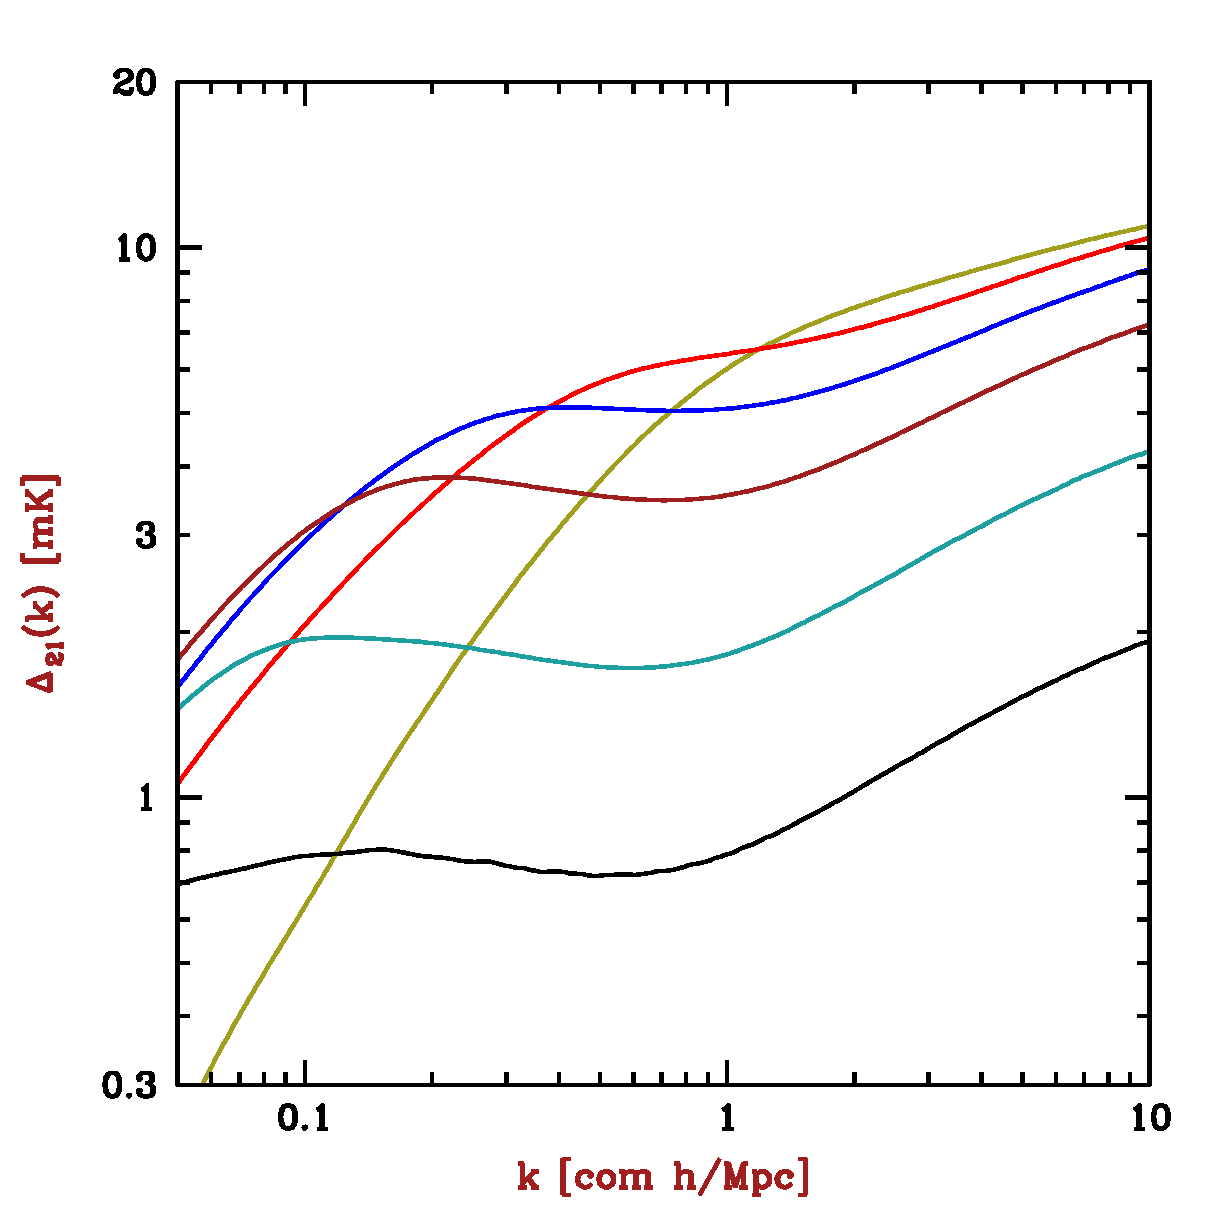
\includegraphics[width=0.45\textwidth]{plots/PS_evolution.eps}
    \caption{The theoretical evolution of the cross-$21$\,cm power spectrum for a specific model (image credit: \citet{barkana2009}), where the neutral fraction $x_{HI} = 10\%, 30\%, 50\%, 70\%, 90\%$, and $98\%$ from top to bottom at large $k$. This figure shows the expected evolution of the power spectrum which interferometers seek to measure.}
    \label{fig:PS_evolution}
\end{figure}

\subsection{Calibration}

We now transition to a brief overview of key data processing steps that are often standard routines when going from visibilities to power spectra. We speak broadly about these steps in this chapter, and go into detail about them for specific experiments in later chapters.

As discussed previously, an interferometer measures a visibility for every baseline pair and every time integration. Repeated baseline types and multi-day observations can be stacked to gain sensitivity to Fourier-modes on the sky. However, ensuring clean measurements at EoR sensitivities requires many other crucial processing steps, including calibration, which we give an overview of in this section.

We've seen that the visibility measurement is dependent on the sky, baseline, and antenna beam, but it is also affected by instrumental systematics. For example, certain components in the signal chain of an instrument can contribute variable noise, losses can arise from reflections, and blockage and scattering may occur. These are all effects that must be considered in order to accurately extract the EoR signal. 

Many of these effects can be mitigated through precise calibration. There are two main types of calibration used by $21$\,cm interferometers: \textit{redundant} calibration and \textit{absolute} calibration. We will briefly describe each here.

Redundant calibration is a type of calibration based on the redundant nature of baselines. For experiments like PAPER and HERA, which have many repeated copies of baselines, redundant calibration can be used to bring all identical baselines into agreement (i.e., it calibrates out deviations between baselines of the same type). This calibration is a powerful technique because it does not use any knowledge of the sky, yet can correct for instrumental-induced gain and phase effects brought on by differences in the signal chain attributable to antennas, cables, and receivers (\citealt{liu_et_al2010}).

Mathematically, the visibility $v_{ij}$ of every baseline can be written as:

\begin{equation}
v_{ij} = g_{i}^{\ast}g_{j}y_{ij} + n_{ij},
\end{equation}
where $g_{i}$ and $g_{j}$ are the complex gains of each antenna, $y_{ij}$ is the ``true" model visibility for that particular baseline type, and $n_{ij}$ is noise. The goal of redundant calibration is to solve for the gain of each antenna and the ``true" visibility of each baseline type. This can be accomplished by setting up a system of linear equations containing every visibility measurement (the method used by PAPER and HERA is detailed in Chapter \ref{sec:PSA64overview}). If there are more measurements than the sum of the number of unique baselines and antennae, then it is a solvable system. 

The complex gains can be further broken down to be written as $g_{i} = e^{\eta_{i} + i\phi_{i}}$ (\citealt{liu_et_al2010}). In other words, by solving for the gains, we are solving for both an amplitude component and a phase offset for each antenna. The gains can then be divided out of every visibility measurement, producing redundantly-calibrated measurements across the whole array.

While redundant calibration is a clever technique for the internal calibration of an interferometer, the calibrated visibility measurements are still on an arbitrary gain scale that has not been matched up to the sky. Hence, absolute calibration refers to using sources in the sky of known brightness (or sky models) in order to solve for the two remaining internal degrees of freedom: an overall gain and an overall phase. Interferometers typically use a standard self-calibration routine to accomplish this, where $y_{ij}$ is known for specific sky sources.

Ultimately, calibration is a crucial step in preparing interferometric data for a power spectrum analysis. A precisely-calibrated instrument will result in cleaner data from which the EoR signal can be accessed.

\subsection{Foreground Filtering}

Arguably the largest challenge of processing $21$\,cm data is in removing bright foregrounds. There are several techniques to do this, which fall into two main categories: foreground subtraction and foreground avoidance. The former consists of modeling and subtracting out foreground sources, while the latter involves making EoR measurements in a domain where foregrounds are minimal. 

For interferometers with imaging capabilities, foreground removal techniques include modeling approaches to spatially localize and remove contaminants (e.g., \citealt{santos_et_al2005}; \citealt{wang_et_al2006}; \citealt{jelic_et_al2008}; \citealt{liu_et_al2009}; \citealt{bowman_et_al2009}; \citealt{harker_et_al2009}; \citealt{chapman_et_al2016}). This can be done by fitting polynomials to data or by using non-parametric methods, which make fewer assumptions about the form of the foregrounds. While foreground subtraction would be ideal if done accurately, modeling is difficult and subtraction poses the risk of cosmological signal loss.

The other method commonly used, foreground avoidance, is a strategy employed by both PAPER and HERA. Foreground avoidance was originally suggested as an alternate method to the subtraction method, which has stringent requirements in order to yield uncontaminated results. In order to understand foreground avoidance, we must first define the ``EoR Window".

A 3D power spectrum can be split into two directions along $k_{\perp}$ and $k_{\parallel}$, which correspond to modes perpendicular to the line-of-sight and along the line-of-sight, respectively. In this two-dimensional space, there are two main regions --- one relatively free of foregrounds (the ``EoR Window") and one contaminated by foregrounds (the ``wedge"), as shown in Figure \ref{fig:wedge} (e.g., \citealt{datta_et_al2010}; \citealt{vedantham_et_al2012}). We can see this by thinking of the $k_{\parallel}$ direction to be akin to the physical time delay associated with light hitting two antennas (a good approximation, especially for short baselines). As $k_{\perp}$, which is proportional to baseline length, increases, the maximum time delay also increases because it is set by the length of the baseline (i.e., a maximum delay occurs when a source is at the horizon; therefore, the time delay is simply the time it takes for the light to travel the distance of the baseline). Hence, the ``wedge" is formed, representing a region where smooth-spectrum foregrounds are expected to be contained. Said differently, foregrounds are expected to be bound by the light-crossing time between two antennas, and therefore there is a maximum limit for $k_{\parallel}$ (time delay) given a $k_{\perp}$ (baseline). 

Delay-filtering is the process by which foregrounds within the wedge are filtered out, leaving a relatively clean window behind from which the cosmological signal can be extracted (\citealt{parsons_et_al2012b}). This approach limits the number of modes for which the measurement can be made and can suffer from some foreground leakage as explained in Chapter \ref{sec:BiasOverview}, but its advantages include its simplicity and conservativeness (i.e., it leaves all the cosmological signal within the window in tact).

\begin{figure}
    \centering
    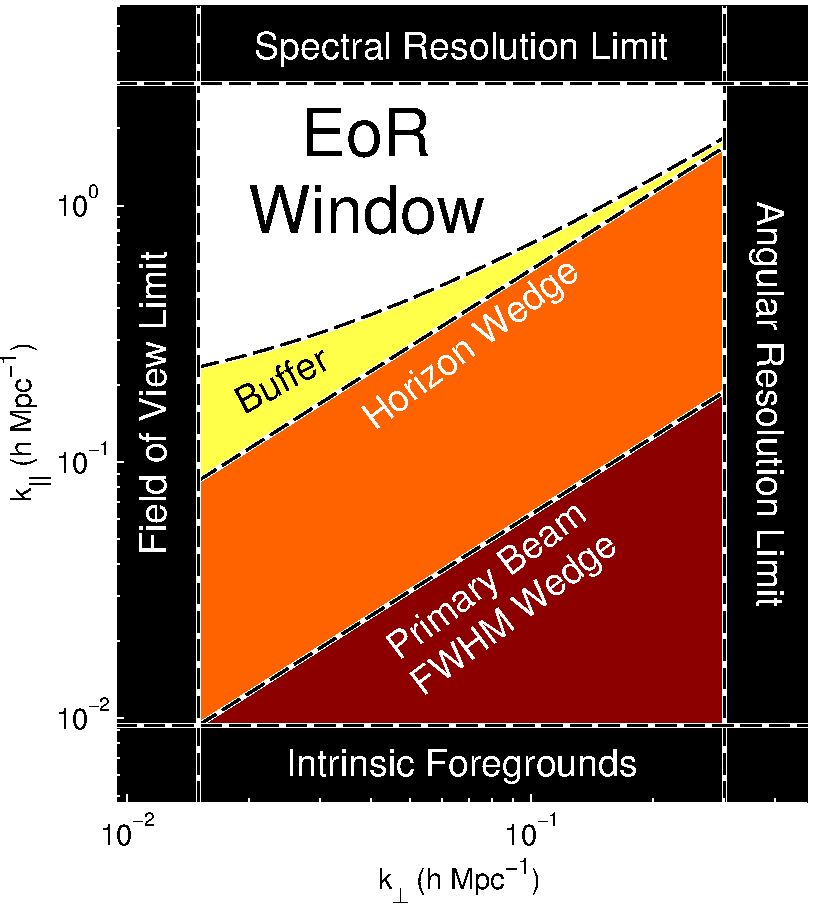
\includegraphics[width=0.45\textwidth]{plots/wedge.pdf}
    \caption{A cartoon diagram of the ``EoR Window" and ``wedge" of foreground contamination in Fourier space (image credit: \citet{dillon_et_al2015b}). A foreground avoidance approach makes power spectrum measurements in the window, while a foreground subtraction approach subtracts out foregrounds so that measurements can be made in the wedge. The overall power spectrum measurement space is limited by an interferometer's field of view and angular resolution along the horizontal axis, and spectral resolution and intrinsic foregrounds along the vertical axis.}
    \label{fig:wedge}
\end{figure}

Whether it's avoidance or removal, there have been many approaches at tackling the challenge of foregrounds (summarized in \citet{chapman_et_al2016}). But, regardless of the method used, removing Galactic and extragalactic foregrounds from $21$\,cm data is absolutely a critical step for analyses seeking the EoR signal. 

\subsection{Fringe-rate Filtering}

The final analysis technique to introduce in this section is fringe-rate filtering, a filtering scheme carried out in a domain which is the Fourier-dual to time. This type of filtering aims to optimize the process of combining time-ordered data and has been investigated in \citet{roshi_perley2003}, \citet{parsons_backer2009}, \citet{offringa_et_al2012}, and \citet{parsons_et_al2016}.

A ``fringe-rate" is the rate at which the sky moves relative to the fringe pattern of an interferometer. As sources pass overhead, they walk in and out of the interference pattern of two antennas, and the rate at which this movement happens is dependent on the source's declination and hour angle. For example, a source located near a celestial pole has a zero fringe-rate, as it does not appear to move in the sky as the Earth rotates. However, a source located on the celestial equator will have a maximum fringe-rate set by the rate of Earth's rotation. The sky can therefore be decomposed into fringe-rate bins, each of which forms a concentric circle of constant fringe-rate around the celestial sphere.

One initial advantage of filtering in fringe-rate space is that it allows the filtering of noise that is not associated with movement locked on the sky (i.e., filtering out fringe-rates greater than the maximum allowed by the Earth's rotation). This excess noise can come from the instrument itself or from signals with an origin not on the sky. Additionally, one can up-weight and down-weight certain portions of the sky by choosing different linear combinations of fringe-rates (\citealt{parsons_et_al2016}). This allows what is effectively a beam-sculpting operation, where the most sensitive parts of one's beam can be up-weighted compared to others.

A third advantage of this type of filtering is that it can also be used to integrate visibilities in time. Depending on the shape of the filter in the fringe-rate domain, the effect in the time domain can be an averaging operation along time. This is advantageous because it allows an optimal way of combining measurements (by weighting fringe-rates differently based on signal-to-noise ratios in each fringe-rate bin, for example) compared to a more traditional boxcar average, which does not use information from individual fringe-rate bins.

Broadly, fringe-rate filtering can be thought of as a tailored filtering step that can increase the sensitivity of a measurement by differentiating between noise- and signal-like modes in data. When carefully chosen, a fringe-rate filter can enhance modes containing emission from the celestial sphere, where the $21$\,cm signal lies.

\section{Instruments}

The recent exploration of our cosmic dawn has led to the development of multiple experiments that are aiming to detect the $21$\,cm signal from neutral hydrogen during reionization. In this section we will first highlight the two main radio interferometers whose data is used in this thesis, and then discuss other similar experiments along with the current status of the field.

\subsection{The Precision Array for Probing the Epoch of Reionization}

The Precision Array for Probing the Epoch of Reionization (PAPER) is a first generation EoR experiment. Its history dates back to 2007, when an initial four dipole antennas observed the sky from Western Australia. A year later, the array increased to eight stations and moved to Green Bank, West Virginia. These first two deployments are summarized in \citet{parsons_et_al2010} and were used to characterize important aspects of the instrument, including system performance, beam models, instrumental temperatures, and sensitivity to radio frequency interference (RFI). 

PAPER then moved to the Karoo Desert in South Africa, near the Square Kilometre Array South Africa (SKA-SA). The PAPER array doubled in size each year, starting with 32 antennas in 2011 and ending with 128 a few years later. PAPER's observing seasons using these three arrays (PAPER-32, PAPER-64, and PAPER-128) have primarily been used to develop analysis techniques, understand instrumental design, and begin to place limits on the EoR and connect them to science implications.

A brief overview of the PAPER instrument and digital backend follows. The PAPER dipole itself (Figure \ref{fig:paper_dipole}) is made from two rods of copper sandwiched between two aluminum disks. The sizes of each are fine-tuned to produce an antenna frequency response between 100-200\,MHz. Each PAPER antenna is sensitive to two orthogonal polarizations, those being the East/West and North/South directions (XX and YY linear polarizations) given the antenna's orientation on the ground. A grounding structure, made of wire-mesh and held in place by PVC pipes, is both underneath the dipole and surrounds it as four angled panels. The design of the antenna's framework was driven by the desire to produce spectrally and spatially smooth beam responses as discussed in \citet{parsons_et_al2010} and \citet{pober_et_al2012}. Altogether, an entire PAPER dipole measures about 2\,m on each side and sits still while the Earth's rotation moves the sky above (``drift-scan" mode). When photons hit the dipoles' copper rods, electrons are excited and their movement turns the electric field into a voltage that can be measured.

\begin{figure}
    \centering
    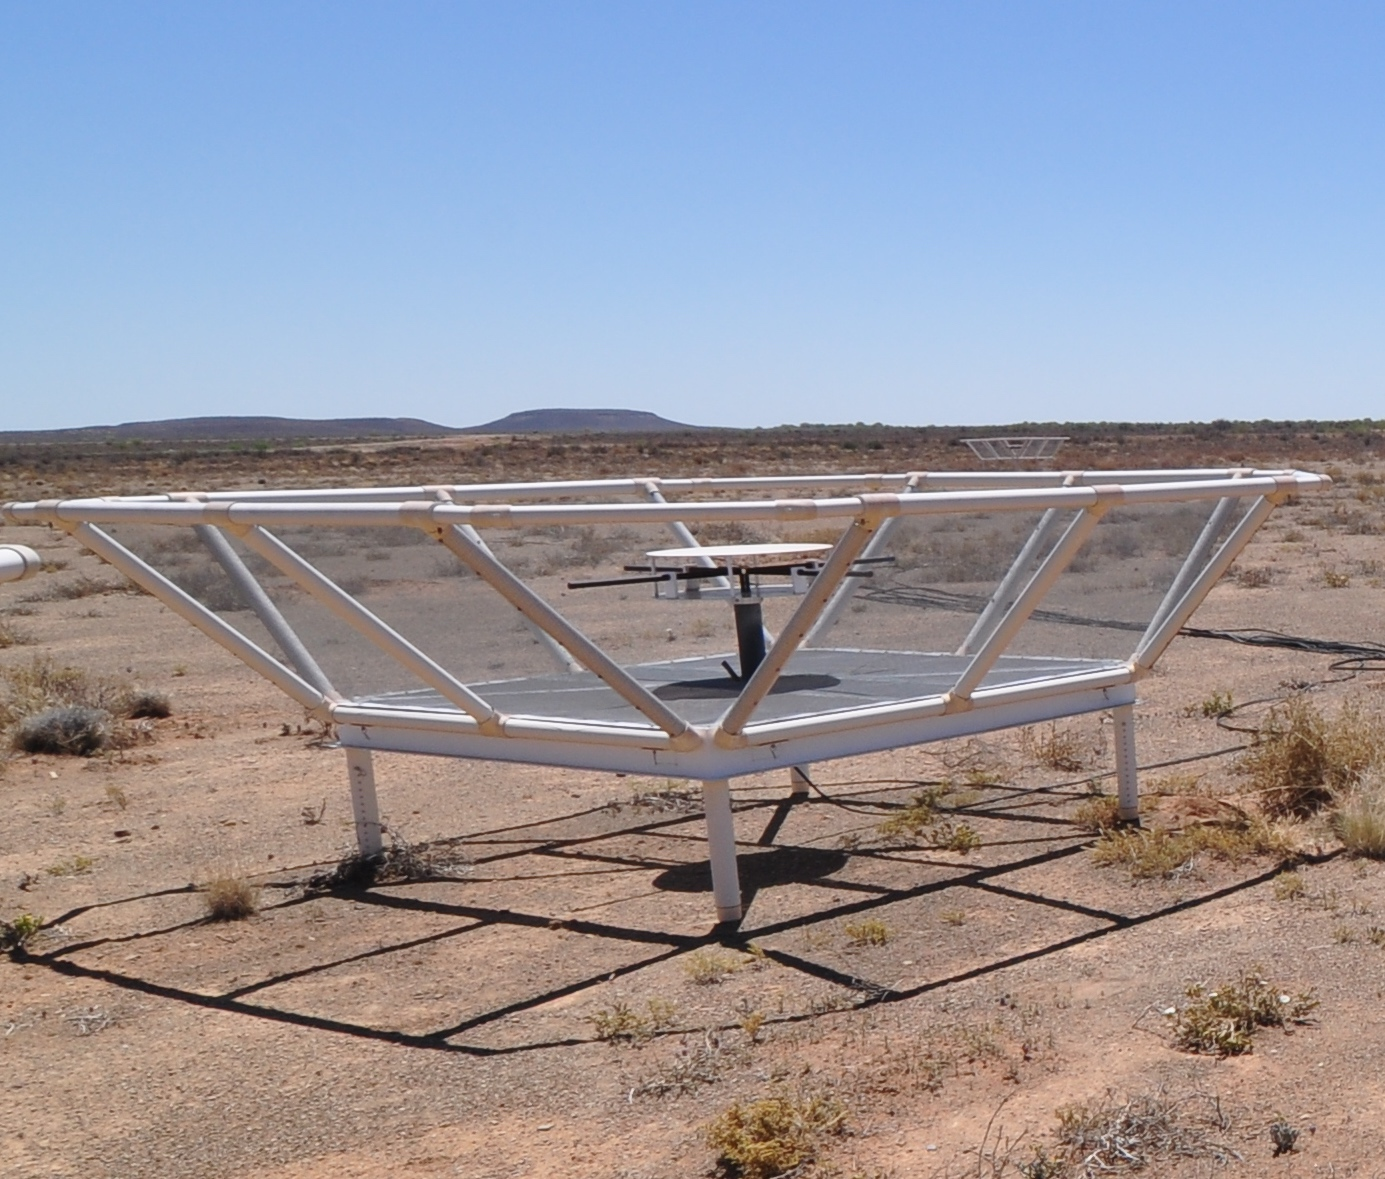
\includegraphics[width=0.5\textwidth]{plots/paper_dipole2.jpg}
    \caption{A PAPER antenna in the Karoo Desert in South Africa. A dual-polarization dipole sits at the center, surrounded by wire mesh panels that measure 2\,m on each side.}
    \label{fig:paper_dipole}
\end{figure}

In short, PAPER's analog system consists of a balun attached to each dipole element (which measures the voltage and amplifies the signal) and coaxial cables which transport the antenna signals. The signals then travel to dual-channel receiver boards which are cooled inside thermal enclosures in order to prevent the introduction of high gains from temperature fluctuations. The receivers both amplify and filter (in frequency) the signals before sending them to the digital system. 

PAPER's digital system is housed inside a refrigerated container on the observing site. The bulk of the processing is carried out by a series of real-time digital FX correlators which cross-correlate pairs of antenna signals to form visibility measurements. More specifically, the FX correlators comprise of ``F-engines" which digitize, down-convert, and channelize antenna inputs, a switch that divides the data into frequency subsets and routes the packets, GPUs which cross-multiply signals from all antenna pairs and integrate in time (``X-engines"), and finally another switch and computer which collect the data, writes it to disk, and sends the final products over an ethernet connection as ``raw" visibility data products that are ready to be analyzed. 

Much of PAPER's digital signal processing (DSP) system has been made possible due to the development of hardware by the Center for Astronomy Signal Processing and Electronics Research (CAPSER). We rely on their Field-programmable Gate Array (FPGA) processors which can quickly perform the fast Fourier-transforms required to produce visibilities. The development of FPGA's into PAPER's DSP system has been critical in allowing for the scalable expansion of the array. 

PAPER's first power spectrum limits on the EoR came from its 32-element array (\citealt{parsons_et_al2014}). PAPER-32 observed in a redundantly-configured layout from 2011-2012, producing a published $2\sigma$ upper limit on the $21$\,cm power spectrum of (41\,mK)$^{2}$ for $k=0.27\, h$\,Mpc$^{-1}$ at $z=7.7$ (\citealt{parsons_et_al2014}). This result, while orders of magnitude above predicted EoR signals, was used to generate constraints on the brightness temperature of $21$\,cm emission for various reionization models and rule out cold reionization scenarios (i.e., some heating of the IGM is necessary by $z=7.7$ to be consistent with PAPER-32's results).

PAPER expanded to 64 elements in 2012, keeping its redundant layout in order to maximize power spectrum sensitivity. The analysis and initial results for PAPER-64's observing season is outlined in \citealt{ali_et_al2015}, where a $2\sigma$ upper limit on the EoR is published as (22\,mK)$^{2}$ for $0.15 < k < 0.5\,h$\,Mpc$^{-1}$ at $z=8.4$. A result at this sensitivity can begin to place more interesting limits on IGM heating models and on the temperature of the IGM during this time (\citealt{pober_et_al2015}).

From 2013-2015, PAPER-128 marked the last era for the PAPER experiment. The data collected with this array has not been published publicly and work is ongoing to process and analyze this data. While most of this thesis focuses on PAPER-64, specifically on analysis methods developed to revise the initial (incorrect) PAPER-64 results (Chapter \ref{c.PSmethods}) and what those new limits should be (Chapter \ref{c.PSA64}), we also present a first-look at PAPER-128 and discuss how PAPER's final observing season has influenced analysis metrics for next generation experiment HERA (Chapter \ref{c.PSA128}).

The PAPER experiment as a whole has been absolutely fundamental to the growth of the field of $21$\,cm cosmology. This first generation experiment set a standard for other similar experiments and has provided countless lessons in all aspects of the signal chain. The array may be retired, but its influence will not be forgotten.

\subsection{The Hydrogen Epoch of Reionization Array}

The development of the Hydrogen Epoch of Reionization Array (HERA) was largely driven by the need for increased sensitivity, as even PAPER-128 lacked the collecting area for a significant detection of the EoR. HERA is a second generation EoR experiment currently being built in the Karoo. It features a staged build-out of parabolic dishes with 14\,m diameters, with construction beginning in 2015 and an eventual 350 dishes planned to be completed by the end of 2019.

A HERA dish (Figure \ref{fig:hera_dish}) is made up of wire-mesh, PVC pipes, and wooden support structures. The size, shape, and total number of the dishes were chosen in order to optimize sensitivity (i.e., minimize chromatic effects that would leak power into the EoR window), minimize costs, and be easily scalable and robust for a five year lifetime (\citealt{deboer_et_al2017}). While work on a new feed design (with a wider bandwidth) is ongoing, the first observations from HERA use recycled PAPER dipoles. Suspended upside-down with a wire pulley-system, the PAPER dipoles are surrounded by a wire-mesh backplane structure that minimizes cross-coupling between antennas while optimizing beam efficiency, frequency response, and polarization match (\citealt{deboer_et_al2017}). Similarly, the first stages of the HERA array are using the existing PAPER signal chain and hardware, while work is progressing towards an underground node-based architecture that will house the DSP system and minimize cable reflections by allowing for shorter cable paths. 

\begin{figure}
    \centering
    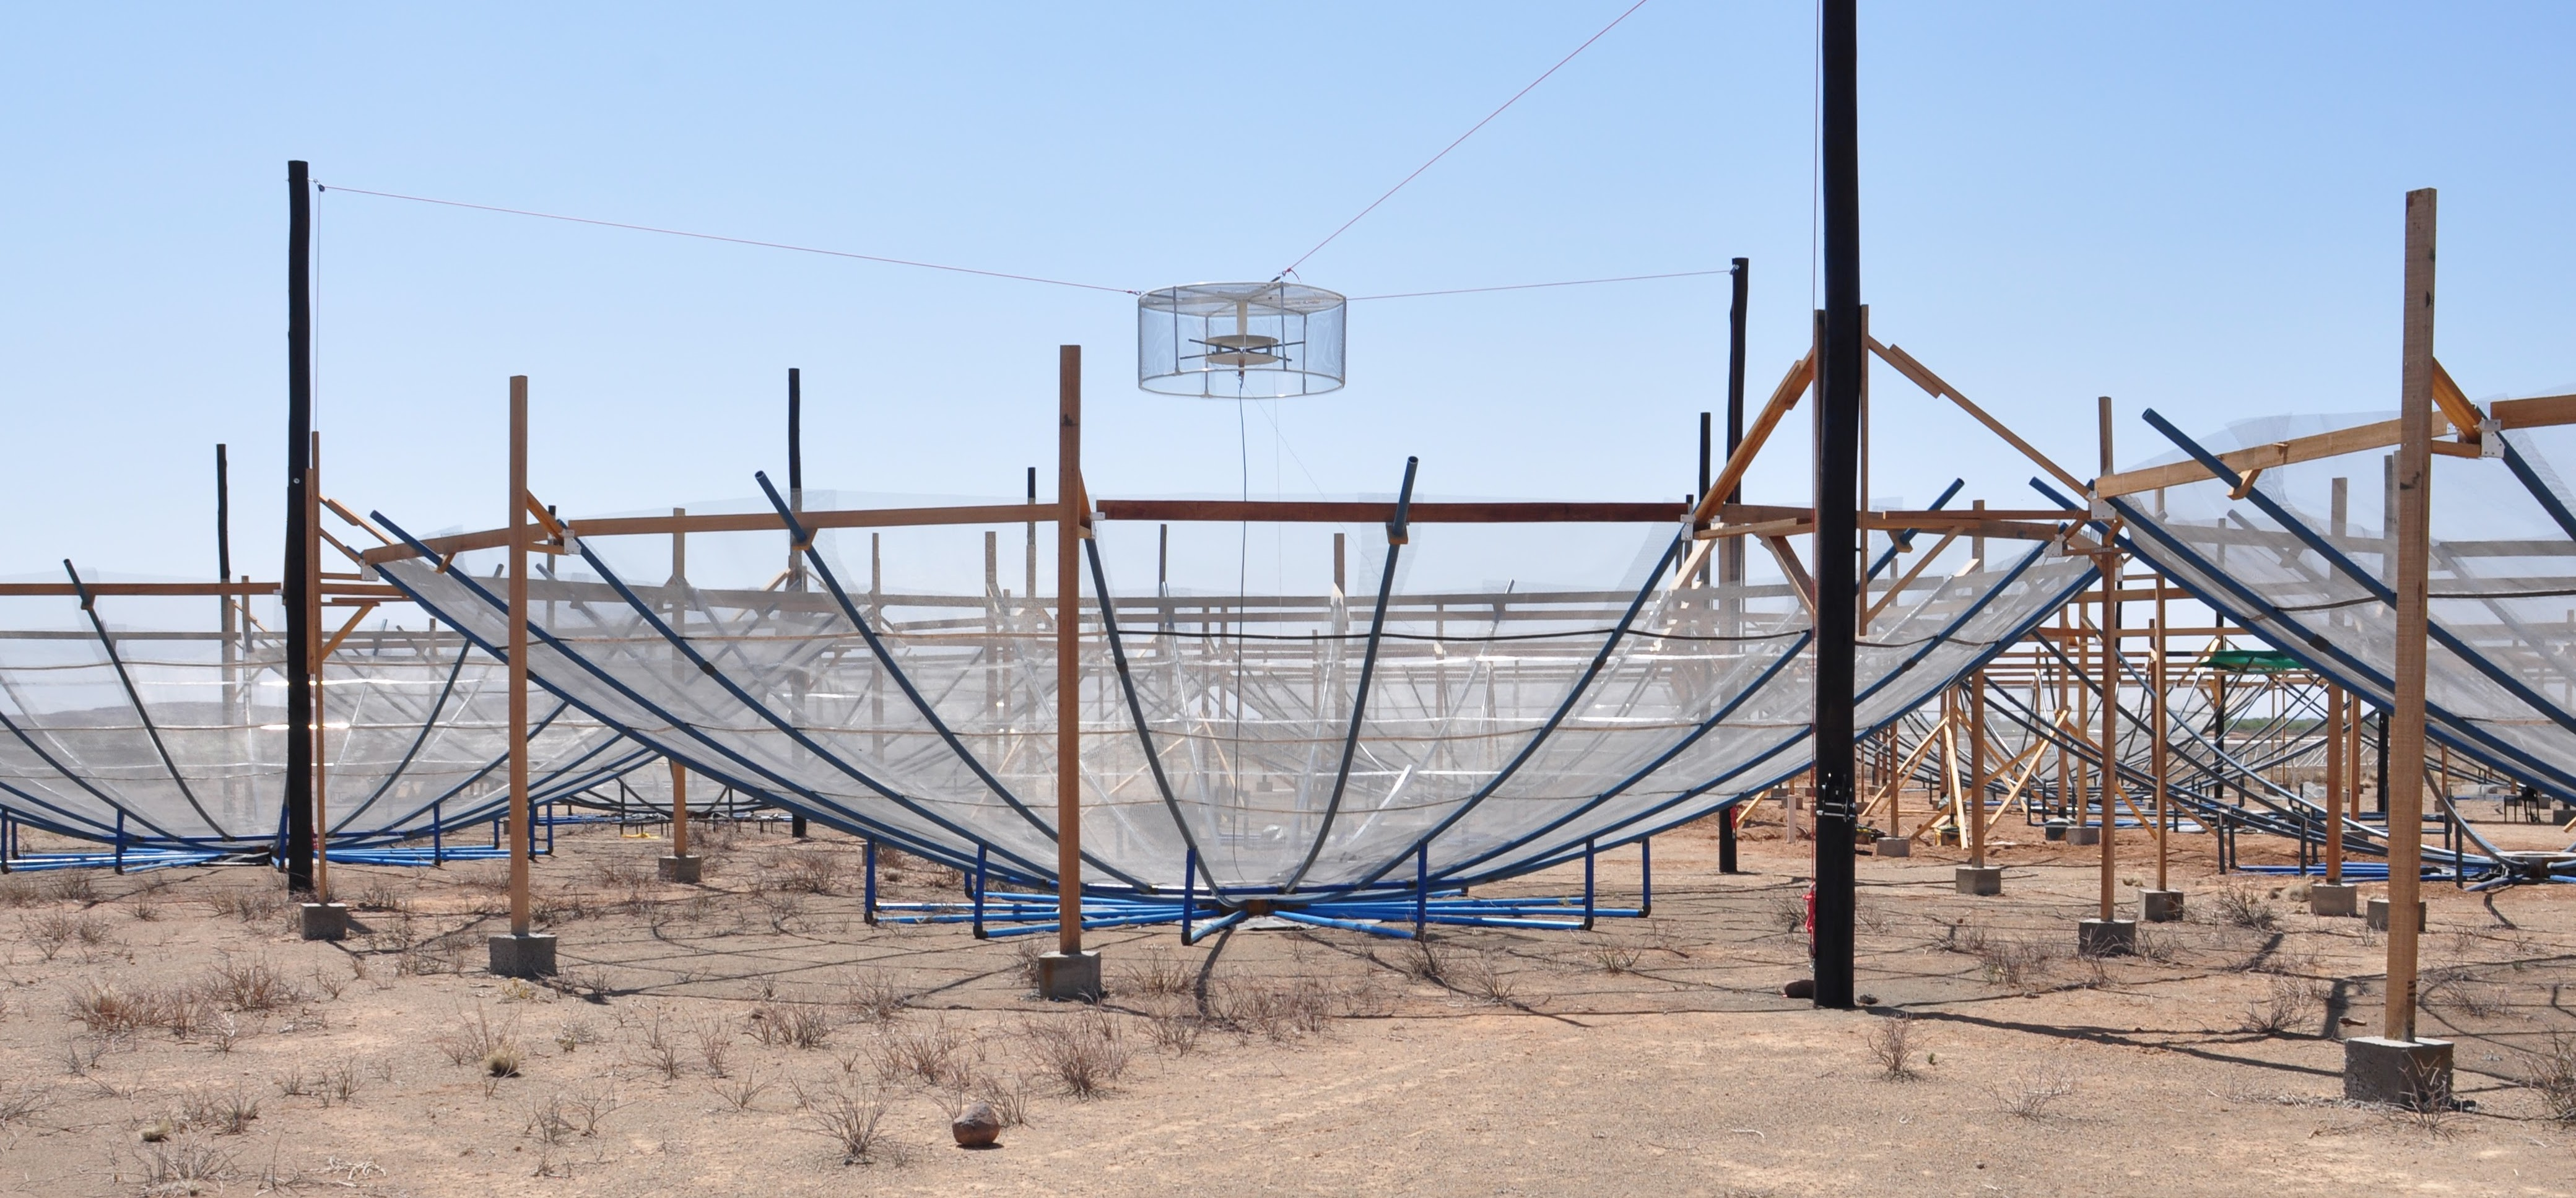
\includegraphics[width=1\textwidth]{plots/hera_dish.jpg}
    \caption{A HERA dish in the Karoo Desert in South Africa. Wire-mesh, PVC pipes, and wooden structures serve as the foundation for the 14\,m diameter parabola. A PAPER dipole is suspended upside-down with a wire pulley-system and surrounded by a prototype wire-mesh skirt structure. HERA-350 will use an updated design for its feed; however, HERA's initial data releases use the old PAPER infrastructure as depicted here.}
    \label{fig:hera_dish}
\end{figure}

The configuration of HERA, like PAPER, is highly redundant and optimized for a robust foreground avoidance approach. Because this power spectrum approach requires short baselines (which minimize the wedge), the HERA antennas are densely-packed next to each other into a main core. This core is segmented into three displaced sections, whose sectioning is designed to improve HERA's imaging ability (\citealt{dillon_parsons2016}). Additionally, there will be 30 outrigger elements joining the full array, allowing for a more complete \textit{uv}-plane coverage and imaging capabilities that can be leveraged for a foreground removal approach. The full HERA array is depicted in Figure \ref{fig:hera_array}. 

\begin{figure}
    \centering
    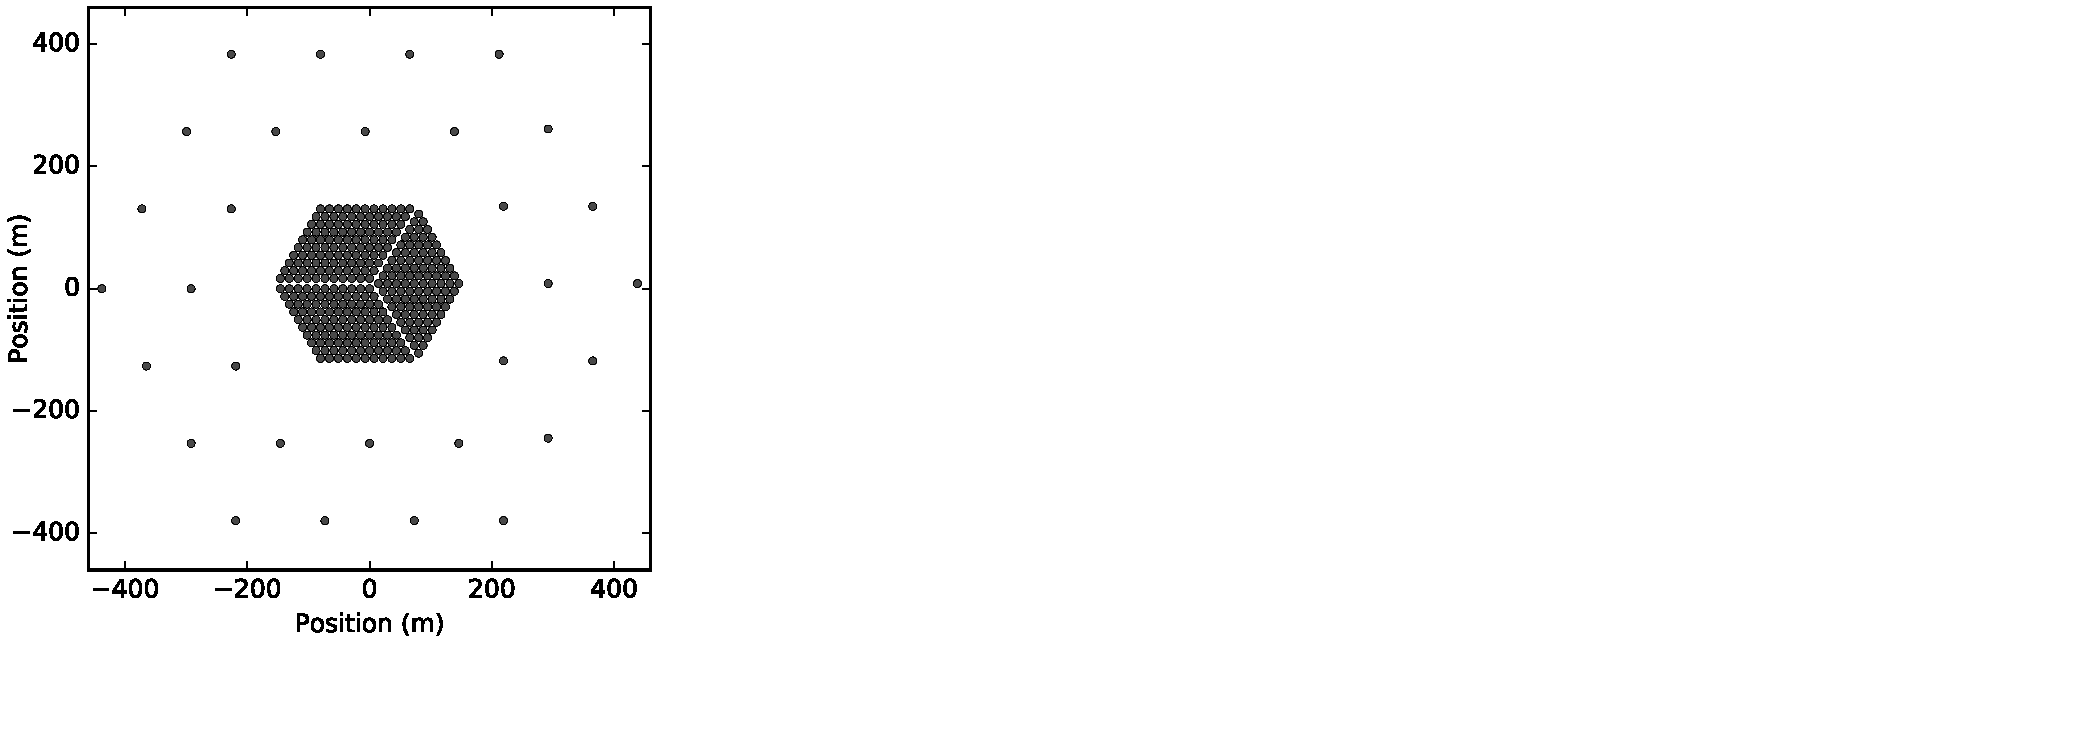
\includegraphics[width=0.5\textwidth]{plots/hera_array.pdf}
    \caption{The full HERA-350 array (image credit: \citet{deboer_et_al2017}). The array is comprised of a segmented densely-packed core (to optimize redundancy for a foreground avoidance approach) and surrounding outrigger elements (for imaging capabilities).}
    \label{fig:hera_array}
\end{figure}

The primary science goal of HERA is to make a high-significance detection of the cosmological signal in order to constrain the timing and morphology of reionization. With precision constraints on the EoR, we can begin to understand the role of the first stars and galaxies in driving reionization, their complex interactions with their environments, and the evolution of cosmic structure. With the full array and an upgraded feed sensitive from 50-250\,MHz, secondary science goals of the instrument include precision cosmology, imaging of the reionization epoch, and an investigation of the pre-reionization heating epoch (\citealt{deboer_et_al2017}). HERA, with a collecting area of $\sim0.1$\,km$^{2}$, is well-poised for these challenges (\citealt{pober_et_al2014}) and has already undergone numerous tests and simulations to ensure that its design meets specification (\citealt{neben_et_al2016}; \citealt{ewall-wice_et_al2017}; \citealt{patra_et_al2018}). As the fully realized HERA soon approaches, there is much to look forward to in the coming years from this array.

\subsection{Other Experiments and Status of Field}

Although this thesis focuses mostly on PAPER data and analysis methods that will be used by HERA, these two arrays are not alone in their quest for the EoR. Other radio interferometers which seek to measure statistical power spectra include the Giant Metre-wave Radio Telescope located in India (GMRT; \citealt{paciga_et_al2013}), the LOw Frequency ARray in Europe (LOFAR; \citealt{van_haarlem_et_al2013}), the Murchison Widefield Array in Australia (MWA; \citealt{tingay_et_al2013}), the 21 Centimeter Array in China (21CMA; \citealt{peterson_et_al2004}; \citealt{wu2009}), and the Square Kilometre Array in South Africa (SKA; \citealt{koopmans_et_al2015}).

Several of these experiments have succeeded in placing upper limits on the EoR, including results from the 32-tile MWA (\citealt{dillon_et_al2014}), 128-tile MWA (\citealt{dillon_et_al2015}; \citealt{beardsley_et_al2016}), GMRT (\citealt{paciga_et_al2013}), and LOFAR (\citealt{patil_et_al2017}). PAPER has also previously published results using 32 antennas (\citealt{parsons_et_al2014}; \citealt{jacobs_et_al2015}) and 64 antennas (\citealt{ali_et_al2015}), though we highlight the errors found in PAPER's analysis pipeline throughout this thesis and thus refer the reader to Chapter \ref{c.PSA64} for updated results from PAPER.

The work in the 21\,cm community that has led to these power spectrum limits (Figure \ref{fig:statusfield}) has largely revolved around the key challenge of controlling foregrounds and systematics. To accomplish this, significant progress has been made in all aspects of the experimental process, ranging from carefully designed interferometers (\citealt{lonsdale_et_al2009}; \citealt{parsons_et_al2012a}; \citealt{dillon_parsons2016}), to novel methods for understanding and dealing with foregrounds (e.g., \citealt{morales_et_al2006}; \citealt{datta_et_al2010}; \citealt{sullivan_et_al2012}; \citealt{moore_et_al2013}; \citealt{hazelton_et_al2013}; \citealt{pober_et_al2013b}; \citealt{liu_et_al2014a}; \citealt{liu_et_al2014b}; \citealt{thyagarajan_et_al2015}), to statistical analysis techniques for precise calibration and power spectrum estimation (e.g., \citealt{liu_et_al2010}; \citealt{trott_et_al2012}; \citealt{liu_et_al2014b}; \citealt{zheng_et_al2014}; \citealt{dillon_et_al2014}; \citealt{jacobs_et_al2016}). PAPER's foreground avoidance strategies have, in particular, led to detailed understandings of redundant calibration and the effects of filtering on the EoR window, while MWA's foreground subtraction techniques have provided complementary improvements in imaging capabilities. While the experiments with published results currently lack the sensitivities needed for an EoR detection, both the delay-filtering and map-making methods, along with hybrid approaches (\citealt{trott_et_al2016}), have set a strong foundation for controlling foregrounds by future, more sensitive interferometers.

Related to the fundamental goal of simultaneously maximizing sensitivity and minimizing contaminants, some other challenges that face current $21$\,cm experiments include polarization leakage from Faraday-rotated emission (\citealt{moore_et_al2013}; \citealt{kohn_et_al2016}; \citealt{nunhokee_et_al2017}), direction-dependent beam effects, and other low level sources of chromaticity induced by the instrument or calibration. These effects will require thorough investigations as experiments approach EoR sensitivities.

\begin{figure}
    \centering
    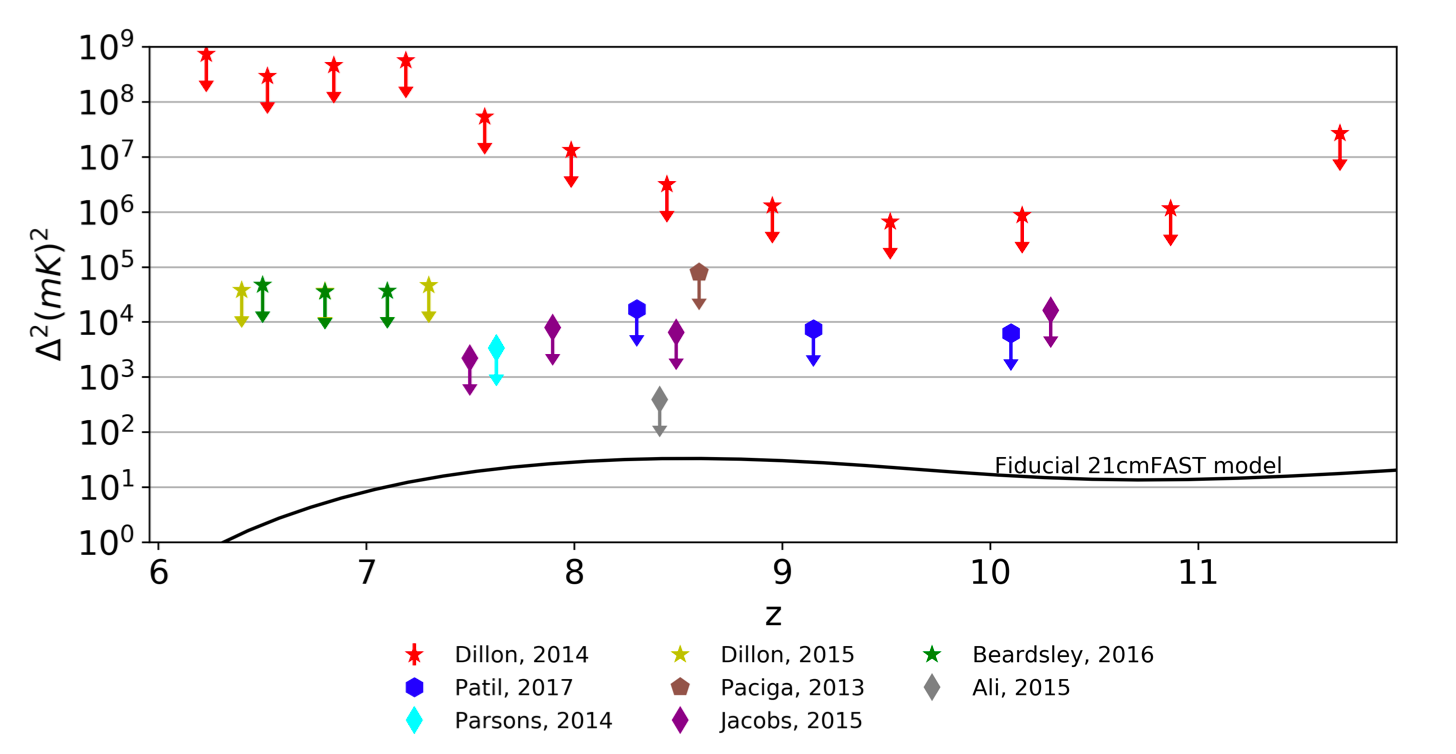
\includegraphics[width=1\textwidth]{plots/statusfield.png}
    \caption{Published upper limits on the EoR placed by different $21$\,cm experiments, prior to the work in this thesis. All PAPER results shown (PAPER-32 is in cyan and magenta, and PAPER-64 is in blue) are suspect to the errors discussed throughout this work and are superseded by the ones presented in Chapter \ref{c.PSA64}.}
    \label{fig:statusfield}
\end{figure}

In addition to power spectrum experiments, there are several complementary experiments that aim to measure the sky-averaged global $21$\,cm signal (i.e., the mean brightness temperature of the EoR relative to the CMB). These include the Experiment to Detect the Global EoR Signature (EDGES; \citealt{bowman2010}), the Large Aperture Experiment to Detect the Dark Ages (LEDA; \citealt{bernardi_et_al2016}), the Dark Ages Radio Explorer (DARE; \citealt{burns2012}), the Sonda Cosmol\'ogica de las Islas para la Detecci\'on de Hidr\'ogeno NeutroSciHi (SCI-HI; \citealt{voytek2014}), the Broadband Instrument for Global HydrOgen ReioNisation Signal (BIGHORNS; \citealt{sokolowski2015}), and the Shaped Antenna measurement of the background RAdio Spectrum (SARAS; \citealt{patra2015}).

Like the power spectrum experiments, global signal experiments also face challenges of bright foregrounds and instrumental systematics. In particular, they require extremely precise calibration in order to avoid overfitting when subtracting foregrounds, and they also face additional challenges when observing the lowest frequencies, such as ionospheric fluctuations and brighter foregrounds (\citealt{vedantham_et_al2014}; \citealt{datta_et_al2014}).

However, most global signal telescopes consist of single elements and can therefore be more easily constructed. Additionally, EoR sensitivities can be reached with relatively short observations. Thus, global signal experiments are actively being worked on as a complementary view into the evolution of the $21$\,cm signal. Accurate detections of the features of the global signal will delineate the different epochs in the early Universe, and their shapes will carry important implications about the nature of the IGM and the first sources.

For example, the first potential detection of the $21$\,cm signal has been made by the global signal experiment EDGES (\citealt{bowman_et_al2018}). This exciting result suggests the presence of an absorption feature in the sky-averaged spectrum at 78\,MHz, thought to be the result of the absorption of CMB photons by HI gas. Because the detected feature is best-fit by an amplitude much larger than what is consistent with expectations for the $21$\,cm signal during this epoch, alternate scientific explanations have been offered, such as the influence of dark matter on baryons and the effect of their interaction on the temperature of the gas (\citealt{barkana2018}; \citealt{slatyer_wu2018}), . Measurements from other experiments in the future will certainly be informative in shaping the community's confidence in this detection, and this result marks just the beginning of many more in the field to come.





\defcitealias{ali_et_al2015}{A15}

\chapter{Power Spectrum Methods}
\label{c.PSmethods}

% change "Chapter" to "Chapter"

\section{Power Spectrum Themes and Techniques}

The major challenge that faces all 21\,cm experiments is isolating a small signal that is buried underneath foregrounds and 
instrumental systematics that are, when combined, four to five orders of magnitude brighter \citep[e.g.,][]{santos_et_al2005, ali_et_al2008, deOliveiraCosta_et_al2008, jelic_et_al2008, bernardi_et_al2009, bernardi_et_al2010, ghosh_et_al2011, pober_et_al2013b, bernardi_et_al2013, dillon_et_al2014, kohn_et_al2016}. A clean measurement therefore requires an intimate understanding of the instrument and a rigorous study of data analysis choices. With continual progress being made 
in the field and HERA on the horizon, it is becoming increasingly important to understand how the methods we choose interact 
with each other to affect power spectrum results. More specifically, it is imperative to develop techniques and tests that ensure 
the accuracy and reliability of a potential EoR detection. In this chapter and the next, we discuss three topics (signal loss, error estimation, and bias) that are essential to investigate 
for a robust 21\,cm power spectrum analysis. We also highlight four power spectrum techniques (fringe-rate filtering, weighting, bootstrapping, jackknife testing) and their trade-offs, potential 
pitfalls, and connections to the themes. We first approach the themes from a broad perspective (Chapter \ref{c.PSmethods}), introducing the themes of our focus and using toy models to develop intuition into each one. We then perform a detailed 
case study (Chapter \ref{c.PSA64}) using data from the 64-element configuration of PAPER, highlighting key changes from the methods used in the previously published result in \citet{ali_et_al2015}, henceforth known as \citetalias{ali_et_al2015}, which have led to a 
revised PAPER-64 power spectrum result. In these two chapters we use a subset of PAPER-64 data to illustrate our revised analysis methods, while Chapter \ref{c.PSA64_results} builds off of the methods to finally present revised PAPER-64 results for multiple redshifts and baseline types.

We note that this thesis as a whole adds to the growing foundations of lessons which have been documented, for example, in \citet{paciga_et_al2013}, \citet{Patil2016}, and \citet{jacobs_et_al2016}, by the GMRT, LOFAR, and MWA projects respectively. These lessons are imperative as the community moves towards higher sensitivities and potential EoR detections.

There are many choices a 21\,cm data analyst must consider. How can time-ordered measurements be combined? How can the 
variance of the data be estimated? In what way(s) can the data be weighted to suppress contaminated modes while not 
destroying an EoR signal? How can a statistically significant detection of a signal be properly identified? Many common techniques, such as 
averaging data, weighting, bootstrapping, and jackknife testing, address these issues but harbor additional trade-offs. For 
example, an aggressive filtering method may succeed in eliminating interfering systematics but comes at the cost of losing 
some EoR signal. A chosen weighting scheme may theoretically maximize sensitivity but fail to suppress foregrounds in practice. 

Though there are many data analysis choices, measuring the statistical 21\,cm power spectrum ultimately requires robust 
methods for determining accurate confidence intervals and rigorous techniques to identify and control systematics.  In this 
thesis, we focus on three 21\,cm power spectrum themes that encapsulate this goal and discuss four techniques that interplay 
with each other and impact the themes. We will give brief definitions now, and build intuition for each theme in the sections to 
follow.

\begin{itemize}
\item \textbf{Signal Loss} (Chapters \ref{sec:SiglossOverview} and \ref{sec:SiglossMath}): Signal loss refers to attenuation of the target \textit{cosmological} signal 
in a power spectrum estimate. Certain analysis techniques can cause this loss, and if the amount of loss is not quantified accurately, it could lead to false non-detections and overly aggressive upper limits. Determining whether an analysis pipeline is lossy, and estimating the amount of loss if so, has subtle challenges but is necessary to ensure the accuracy of any result. 
\item \textbf{Error Estimation} (Chapter \ref{sec:ErrorOverview}): Confidence intervals on a 21\,cm power spectrum result 
determine the difference between a detection and a null result, which have two very different implications. Additionally, accurate error estimation is crucial for the comparison of results to theoretical models. Errors can be 
estimated in a variety of ways, and we will discuss a few of them.
\item \textbf{Bias} (Chapter \ref{sec:BiasOverview}): There are several possible sources of power offset in a visibility 
measurement that can show up as a detection in a power spectrum, such as bias from noise and foregrounds. In particular, a 
successful EoR detection would also imitate a bias. Proving that a bias is an EoR detection may be the most difficult challenge for future 21\,cm 
analyses, as it is crucial to be able to distinguish a detection of foreground leakage, for example, from that of EoR. In this chapter,
we will highlight some sources of bias, discuss ways to mitigate their effects, and describe example tests that a true EoR detection must 
pass.
\end{itemize}

The following techniques each have advantages when it comes to maximizing sensitivity and understanding systematics in 
data. However, some have limitations, and we will discuss circumstances in which there are trade-offs. We choose to focus on 
these four techniques because they represent major steps in PAPER's power spectrum pipeline, with several of them also 
being standard steps in general 21\,cm analyses.
\begin{itemize}
\item \textbf{Fringe-rate filtering:} Fringe-rate filtering is an averaging scheme for time-ordered data 
(\citealt{parsons_et_al2016}). Broadly, a fringe-rate filter, as described in more detail in Chapter \ref{sec:frf_intro}, averages visibilities in time to produce a smaller number of more sensitive 
independent samples. However, such a filter also affects the presence 
of foregrounds and systematics. We explain the trade-offs of filtering in more detail in Chapter \ref{sec:toymodel_frf}.
\item \textbf{Weighting:} A data set can be weighted to emphasize certain features and minimize others. One particular flavor of 
weighting employed by previous PAPER analyses is inverse covariance weighting in frequency, which is a generalized version of inverse variance 
weighting that also takes into account frequency correlations (\citealt{liu_tegmark2011}; \citealt{dillon_et_al2013a}; \citealt{liu_et_al2014a}; \citealt{liu_et_al2014b}; \citealt{dillon_et_al2014}; \citealt{dillon_et_al2015}). Using such a technique enables the down-weighting of contaminant modes that obey a different covariance structure from that of cosmological modes. However, a challenge of inverse covariance 
weighting is in estimating a covariance matrix that is closest to the true covariance of the data; the discrepancy between the two can have large impacts on signal loss. We investigate the impact of different types of weighting on signal loss in Chapter \ref{sec:SiglossOverview}.
\item \textbf{Bootstrapping:} In addition to using theoretical models for covariance matrices and theoretical error estimation 
methods, bootstrapping is one way to estimate errors. Namely, bootstrapping is a useful method for estimating errors of a data set from 
itself (\citealt{andrae2010}). By randomly drawing many subsamples of the data, we obtain a sense of its inherent variance, though there are subtleties to 
consider such as the independence of values in a data set. We explore this potential pitfall of bootstrapping in Chapter \ref{sec:ErrorOverview}.
\item \textbf{Jackknife testing:} A resampling technique useful for estimating bias, jackknives can be taken along different 
dimensions of a data set to cross-validate results. In particular, null tests can be used to verify whether results are free of 
systematics, as done with CO power spectra (\citealt{keating_et_al2016}) and CMB measurements (see e.g., \citealt{ade_et_al2008}; \citealt{chiang_et_al2010}; \citealt{bischoff_et_al2011}; \citealt{das_et_al2011b}; \citealt{araujo_et_al2012}; \citealt{crites_et_al2015}; \citealt{ade_et_al2016}; \citealt{ade_et_al2017}; \citealt{sherwin_et_al2017}). An EoR detection must pass both jackknife and null tests, which we highlight in Chapter \ref{sec:JackknifeOverview}.
\end{itemize}

In this chapter, we study each theme in depth, focusing on how power spectrum technique trade-offs affect each. 
We use toy data models to develop intuition into why certain analysis choices may be appealing and discuss ways in which 
they are limited. We highlight problems that can arise regarding each theme and offer suggestions to mitigate the issues. 
Ultimately, we show that rigorous investigations into signal loss, error estimation, and bias must be performed for robust 21\,cm results.

\section{Signal Loss Toy Model}
\label{sec:SiglossOverview}

Signal loss can arise in a variety of ways in an analysis pipeline, such as by fitting a polynomial during spectral calibration, applying a delay domain filter, or deriving weights from data and applying them to itself. Here we focus on signal loss associated with 
% JEA - we're not considering a general problem, but are really just focused on the empirical QE and its discontents, so let's say that
the use of an empirically estimated covariance matrix with the "optimal quadratic estimator'' formalism.
This loss was significantly 
%applying a weighting matrix to data, a loss that can be significant depending on the choice of weighting and one that was previously 
underestimated in the \citetalias{ali_et_al2015} analysis.

\subsection{The Quadratic Estimator Method}
\label{sec:QE}

%AAAICW

We begin with an overview of the quadratic estimator (QE) formalism used for power spectrum estimation. The goal of power spectrum analysis is to produce an unbiased estimator of the EoR power spectrum in the presence of both noise and foreground emission. Prior to power spectrum estimation, the data will often have been prepared to have minimal foregrounds by some method of subtraction, so this foreground emission may appear either directly (because it was not subtracted) or as a residual of some subtraction process not in the power spectrum domain. If an accurate estimate of the total covariance of the data is known, including both the desired signal and any contaminants, then the "optimal quadratic estimator" formalism provides a method of producing a minimum variance, unbiased estimator of the desired signal, as shown in 
% JEA - I cut this b/c I wanted to step back and explain a bit more clearly what we were actually hoping for 
%Driven by the need to mitigate foreground bias, PAPER's previous analyses use a weighting method that aims to down-weight foregrounds. This weighting is applied to data, which is then propagated into a final estimator using the power spectrum estimation technique of quadratic estimators (QE) as done in 
\citet{liu_tegmark2011}, \citet{dillon_et_al2013a}, \citet{liu_et_al2014a}, \citet{liu_et_al2014b}, \citet{trott_et_al2012}, \citet{dillon_et_al2014}, \citet{dillon_et_al2015}, \citet{switzer_et_al2015}, and \citet{trott_et_al2016}. 
%Before showing how signal loss can arise when using different weighting matrices, we first summarize QE as performed in the PAPER analysis.

% JEA - The discussion of dimensions here is confusing ... "a baseline" is mentioned, but it's not clear if the redundant baseline averaging has already happened or what.  I believe we are only considering covariance between frequencies, but this isn't explicitly said, and the matrix equations don't make sense unless all the dimensions are N_f N_t.  
%We begin with our 
Suppose that the measured visibilities for a single baseline in Jy are arranged as a data vector, $\textbf{x}$. It has length $N_{t} N_{f}$,
% JEA - not sure this helps
%, but in practice we manipulate it as an array with dimensions ($N_{f}, N_{t}$), 
where $N_{t}$ is the number of time integrations and $N_{f}$ is the number of frequency channels. The covariance of the data is given by 
\begin{equation}
\textbf{C} \equiv \langle\textbf{xx}^{\dagger}\rangle = \textbf{S} + \textbf{U}
\end{equation}
where the average over an ensemble of data realizations produces the true covariance, and we further assume it may be written as the sum of the desired cosmological signal $\textbf{S}$ and other terms $\textbf{U}$.  

We are interested in estimating the three-dimensional power spectrum of the EoR.  
Visibilities are measurements of the Fourier transform of the sky along two spatial dimensions (using the flat-sky approximation), and since we are interested in three-dimensional Fourier modes we only need to take one Fourier transform of our visibilities along the line-of-sight dimension.  We consider band powers $P^\alpha$ of the power spectrum of $\textbf{x}$ over some range in cosmological $\mathbf{k}$, where $\alpha$ indexes a waveband in $k_{\parallel}$ (a cosmological wavenumber $k_{\parallel}$ is the Fourier dual to frequency under the delay approximation (\citealt{parsons_et_al2012b}), which is a good approximation for the short baselines that PAPER analyzes).  The fundamental dependence of the covariance on the power spectrum band powers $P^\alpha$ is encoded as 
% JEA - Should distinguish slightly more clearly between Q and dC/dp_alpha
\begin{equation}
\textbf{S} = \sum_\alpha P^\alpha \frac{\partial\textbf{C}}{\partial P^\alpha} \equiv \sum_\alpha P^\alpha \textbf{Q}^\alpha
%\textbf{S} = p_{\alpha} \frac{\partial\textbf{C}}{\partial p_{\alpha}}
%\frac{\partial\textbf{C}}{\partial p_{\alpha}} \equiv \textbf{Q}^{\alpha}
\end{equation}
where we define $\frac{\partial\textbf{C}}{\partial P^\alpha} \equiv \textbf{Q}^{\alpha}$. In other words, $\textbf{Q}$ describes the response of the covariance to a change in the power spectrum, relating a quadratic statistic of the data (the covariance) to a quadratic statistic in Fourier-space (the power spectrum). 
% JEA - ah, the dimensions again
% which has dimensions ($N_{f}$,$N_{f}$).

The optimal quadratic estimator prescription is then to compute
\begin{equation}
\label{eq:OQE}
\widehat{P}^{\alpha}  = \sum_\beta ({\F^{-1}})^{\alpha\beta} (\widehat{q}^{\beta} - \widehat{b}^{\beta} )
\end{equation}
where $\F$ is the Fisher matrix (which determines errors on the power spectrum estimate)
\begin{equation}
F^{\alpha \beta} \equiv \frac{1}{2} \textrm{tr} \left( \C^{-1} \textbf{Q}^{\alpha} \C^{-1} \textbf{Q}^{\beta} \right),
\end{equation}
$\widehat{q}$ is the un-normalized power spectrum estimate
\begin{equation}
\label{eq:OQEQuadratic}
\widehat{q}^\alpha =  \half \textbf{x}^\dagger \invC \textbf{Q}^{\alpha}  \invC \textbf{x},
\end{equation}
and $\widehat{b}$ is the additive bias
\begin{equation}
\label{eq:OQELinear}
\widehat{b}^{\alpha} = \half \Tr\left( \mathbf{U} \invC \textbf{Q}^{\alpha} \invC \right).
\end{equation}
The power spectrum estimator in Equation \eqref{eq:OQE} is the minimum variance (smallest error bar) estimate of the power spectrum subject to the constraint that it is also unbiased; that is, the ensemble average of the estimator is equal to its true value
\begin{equation}
\label{eq:super_unbiased}
\langle \widehat{P}^{\alpha} \rangle = P^\alpha
\end{equation}
\citep{tegmark_et_al1997a,bond_et_al1998}.

Intuitively, the estimator must be capable of "suppressing" or "removing" the effects of contaminants in order to obtain an unbiased estimate of the power spectrum. By construction, the subtraction of the residual foreground and noise bias accomplishes this, removing any additive bias. However, the $\mathbf{C}^{-1}$ piece of Equation \eqref{eq:OQEQuadratic} also has the effect of suppressing residual foregrounds and noise, in both the additive bias and any contributions the residuals may have to the variance. The way in which the optimal estimator accomplishes this is illustrated with a toy model in Chapter \ref{sec:icw_appendix}. There, we show that the effect of the weighting in Equation \ref{eq:OQEQuadratic} is to project out the modes of $\textbf{U}$ with a different covariance structure than $\mathbf{S}$ in the power spectrum estimate, and the effect of Equation \ref{eq:OQELinear} is to subtract out the remaining bias. Similar effects for a realistic model of the EoR and foregrounds are shown in \citet{liu_tegmark2011}.

The toy model in Chapter \ref{sec:icw_appendix} also illustrates that if the covariance structure of the contaminants is sufficiently different from the desired power spectrum, then the linear bias term may be expected to be quite small, and it is only necessary to know $\C$ and $\textbf{Q}^{\alpha}$, but not $\mathbf{U}$. Since the foregrounds are expected to be strongly correlated between frequencies whereas the EoR is not, we expect different covariance structures and therefore a small linear bias. Moreover, because the linear bias is always positive and there is no multiplicative bias, the quadratic-only term will always produce an estimate which is {\it high} relative to the true value, and which can conservatively be interpreted as an upper limit. These considerations, and the difficulty of obtaining an estimate for $\mathbf{U}$, motivate the neglect of the linear bias in the rest of this analysis.

%We do this when forming the un-normalized power spectrum estimate $\widehat{q}_{\alpha}$:
Motivated by the desire to retain the advantageous behavior of suppressing contributions of $\mathbf{U}$ to estimates of the EoR power spectrum, we note that is possible to define a modified version of the quadratic estimator 
%which may still produce an unbiased estimate, 
where Equation \eqref{eq:OQEQuadratic} is replaced by
\begin{equation}
\label{eq:qhat}
\widehat{q}^{\alpha} = \frac{1}{2}\textbf{x}^{\dagger}\textbf{R}\textbf{Q}^{\alpha}\textbf{R}\textbf{x}
\end{equation}
where $\textbf{R}$ is a weighting matrix chosen by the data analyst.  For example, inverse covariance weighting (the optimal form of QE) would set $\textbf{R} \equiv \textbf{C}^{-1}$ and a uniform-weighted case would use $\textbf{R} \equiv \textbf{I}$, the identity matrix.
Again, the matrix $\textbf{Q}^{\alpha}$ encodes the dependence of the covariance on the power spectrum but in practice also also does other things, including implementing a transform of the frequency domain visibilities to $\mathbf{k}$-space, taking into account cosmological scalings, and converting the visibilities from Jansky to Kelvin.
%with dimensions ($N_{f}$,$N_{f}$) --- as 

%%% COME BACK HERE
% Need to still explain the motivation for this
With an appropriate normalization matrix $\textbf{M}$, the quantity
%We normalize our power spectrum estimates using the matrix $\textbf{M}$:
\begin{equation}
\label{eq:phat}
\widehat{\textbf{P}} = \textbf{M}\widehat{\textbf{q}}
\end{equation}
is a sensible \textit{estimate} of the \textit{true} power spectrum $\textbf{P}$. 

To ensure that $\textbf{M}$ correctly normalizes our power spectrum, one may take the expectation value of Equation \eqref{eq:phat} to obtain
\begin{eqnarray}
\langle \widehat{P}^\alpha \rangle &=& \frac{1}{2} \sum_{\beta \gamma} M^{\alpha \gamma}  \textrm{tr} \left( \textbf{R}\textbf{Q}^{\gamma}\textbf{R} \textbf{Q}^{\beta}\right) P^\beta +\frac{1}{2} \sum_{ \gamma}  \Tr\left( \mathbf{U} \textbf{R} \textbf{Q}^{\gamma} \mathbf{R} \right) \nonumber \\
&\equiv & \sum_{\beta} W^{\alpha \beta} P^\beta +\frac{1}{2} \sum_{ \gamma}  \Tr\left( \mathbf{U} \textbf{R} \textbf{Q}^{\gamma} \mathbf{R} \right), \label{eq:Wpplusbias}
\end{eqnarray}
where $W^{\alpha \beta}$ are elements of a window function matrix. Considering the first term of this expression (again, we are assuming that the linear bias term is significantly suppressed; and if this is not the case, we are simply assuming that we are setting a conservative upper limit), if $\mathbf{W}$ ends up being the identity matrix for our choices of $\mathbf{R}$ and $\mathbf{M}$, then we recover Equation \eqref{eq:super_unbiased} for the first term, and we have an estimator that has no multiplicative matrix bias. However, Equation \eqref{eq:super_unbiased} is a rather restrictive condition, and it is possible to violate it and still have a sensible (and correctly normalized) power spectrum estimate. In particular, as long as the rows of $\mathbf{W}$ sum to unity, our power spectrum will be correctly normalized. Beyond this, the data analyst has a choice for $
\textbf{M}$, and for simplicity throughout this thesis we choose $\textbf{M}$ to be diagonal. In a preview of what is to come, we also stress that the derivation that leads to Equation \eqref{eq:Wpplusbias} assumes that $\mathbf{R}$ and $\mathbf{x}$ are not correlated. If this assumption is violated, a simple application of the (now incorrect) formulae in this section can result in an improperly normalized power spectrum estimator that does not conserve power, i.e., one that has signal loss.
% JEA - is one really free to choose M and R independently?

% JEA - I don't think it's attractive at all
%Without a perfect model for the covariance matrix $\textbf{C}$ of our data, one attractive way to estimate it is to empirically derive it from the data $\textbf{x}$ itself. 
Given the advantages of inverse covariance weighting, a question arises of how one goes about estimating $\C$.  One method is to empirically derive it from the data $\textbf{x}$ itself.
Similar types of weightings that are based on variance information in data are done in \citet{chang_et_al2010} and \citet{switzer_et_al2015}. In previous PAPER analyses, one time-averages the data to obtain:
\begin{equation}
\widehat{\textbf{C}} \equiv \langle\textbf{xx}^{\dagger}\rangle_{t} \approx \langle  \textbf{xx}^{\dagger}\rangle,
\end{equation}
assuming $\langle\textbf{x}\rangle_{t} = 0$ (a reasonable assumption since fringes average to zero over a sufficient 
amount of time), where $\langle \rangle_{t}$ denotes a finite average over time. The weighting matrix for our empirically estimated inverse covariance weighting is then $
\textbf{R} \equiv \widehat{\textbf{C}}^{-1}$, where we use a hat symbol to distinguish the empirical covariance from the true covariance $\textbf{C}$.

In the next three sections, we use toy models to investigate the effects of weighting matrices on signal loss by experimenting with different matrices $\textbf{R}$ and examining their impact on the resulting power spectrum estimates $\widehat{\textbf{P}}$. Our goal in experimenting with weighting is to suppress foregrounds and investigate EoR losses associated with it. We note that we purposely take a thorough and pedagogical approach to describing the toy model examples given in the next few sections. The specifics of how signal loss appears in PAPER's analysis is later described in Chapter \ref{c.PSA64}.

%\item While the correct covariance will remove this contamination, there is no particular harm in having these modes be strongly correlated with the data, since we desire their projection in any case.  

As a brief preview, we summarize our findings in the following sections here:

\begin{itemize}

\item If the covariance matrix is estimated from the data, a strong correlation between the estimated modes and the data will in general produce an estimate of the signal power spectrum which is strongly biased {\it low} relative to the true value.  In this context, this is what we call "signal loss''  (Chapter \ref{sec:toymodel}).

\item The effect of the bias is worsened when the number of independent samples used to estimate the covariance matrix is reduced (Chapter \ref{sec:toymodel_frf}).

\item The rate at which empirical eigenvectors converge to their true forms depends on the sample variance in the empirical estimate and the shape of the empirical eigenspectrum. In general, larger sample variances lead to more loss (Chapter \ref{sec:toymodel_frf}).

%\item The convergence of the modes of the empirical covariance matrix to the true matrix depends on the size of the eigenvalues, with the modes with the largest eigenvalues converging more quickly (in norm) to the true eigenvector than those with smaller eigenvalues. Thus, in estimating the covariance matrix empirically, larger eigenvalue modes are likely to be more reliable (Chapter \ref{sec:toymodel_frf}).

\item Knowing these things, there are some simple ways of altering the empirical covariance matrix to decouple it from the data and produce unbiased power spectrum estimates (Chapter \ref{sec:otherweight}).

% JEA - I really struggle with whether this is intuitively obvious ... it's hard to get a sense of what "noise" is averaging down slower.  All modes have the same number of samples going into the estimate.  Should I think of the size of he eigenvalue is an estimate of its "signal/noise" in the given data realization? 
% Also, have we shown this sufficiently rigorously?  Is the toy model sufficiently general?  (Probably.)  But, for any data set you kind of have to make a decision about where you think "reliable" is, i.e., where in eigenvalue would you make a cut?  Is Figure 20 basically trying to argue for the real data that this is ~a few modes?

\end{itemize}


\subsection{Empirical Inverse Covariance Weighting}
\label{sec:toymodel}

% JEA  - This material was moved up
%One choice for the weighting matrix $\textbf{R}$ used in power spectrum analysis is an inverse covariance matrix. This type of weighting is attractive for power spectrum analyses because it yields the smallest possible error bars on a measurement. Said differently, it gives the minimum variance estimate of the power spectrum (\citealt{tegmark_et_al1997a}; \citealt{bond_et_al1998}). In \citet{liu_tegmark2011}, it was shown that inverse covariance weighting also serves as a way to down-weight some portion of foregrounds (namely, those which do not share the same covariance structure as the cosmological signal), motivating our use of the weighting for previous PAPER analyses.
%
%One important feature of weighting data by its true inverse covariance is that, while it can suppress some foregrounds, it cannot suppress the EoR signal (nor foreground modes that masquerade as signal-like modes). By construction, inverse covariance weighting in the quadratic estimator does not lead to signal loss. Therefore, in an ideal world with perfect foreground, 
%instrumental, and EoR models, we could form $\textbf{C}$ in a way that accurately describes our measured data and use inverse covariance weighting to produce minimum variance power spectrum estimates without destroying the signal. In other words, the optimal quadratic estimator is by construction an unbiased estimator of the power spectrum.

%In practice, we do not have perfect models for $\textbf{C}$, and it is the use of an estimated covariance $\widehat{\textbf{C}}$ instead of the true covariance $\textbf{C}$ that can lead to loss. 
Using a toy model, we will now build intuition into how weighting by the inverse of the empirically estimated covariance, $\widehat{\textbf{C}}^{-1}$, can give rise to signal loss.  We construct a simple data set that contains visibility data with $100$ time integrations and $20$ frequency channels. This model represents realistic dimensions of about an hour of PAPER data which might be used for a power spectrum analysis. For PAPER-64 (both the \citetalias{ali_et_al2015} analysis and our new analysis) we use $\sim8$ hours of data (with channel widths of $0.5$ MHz and integration times of $43$ seconds), but here we scale it down with no loss of generality. 

We create mock visibilities, $\textbf{x}$, and assume a non-tracking, drift-scan observation. Hence, flat spectrum sources (away from zenith) lead to measured visibilities which oscillate in time and frequency. We therefore form a mock visibility measurement of a bright foreground signal, $\textbf{x}_{\rm FG}$, as a complex sinusoid that varies smoothly in time and frequency, a simplistic but realistic representation of a single bright source. We also create a mock visibility measurement of an EoR signal $\textbf{x}_{\rm EoR}$ as a complex, Gaussian random signal. A more realistic EoR signal would have a sloped power spectrum in $p(k)$ (instead of flat, as in the case of white noise), which could be simulated by introducing frequency correlations into the mock EoR signal. However, here we treat all $k$'s separately, so a simplistic white noise approximation can be used. Our combined data vector is then $\textbf{x} = 
\textbf{x}_{\rm FG} + \textbf{x}_{\rm EoR}$, to which we apply different weighting schemes throughout Chapter \ref{sec:SiglossOverview}. The three data components are shown in Figure 
\ref{fig:toy_sigloss1}. 

\begin{figure}
	\centering
	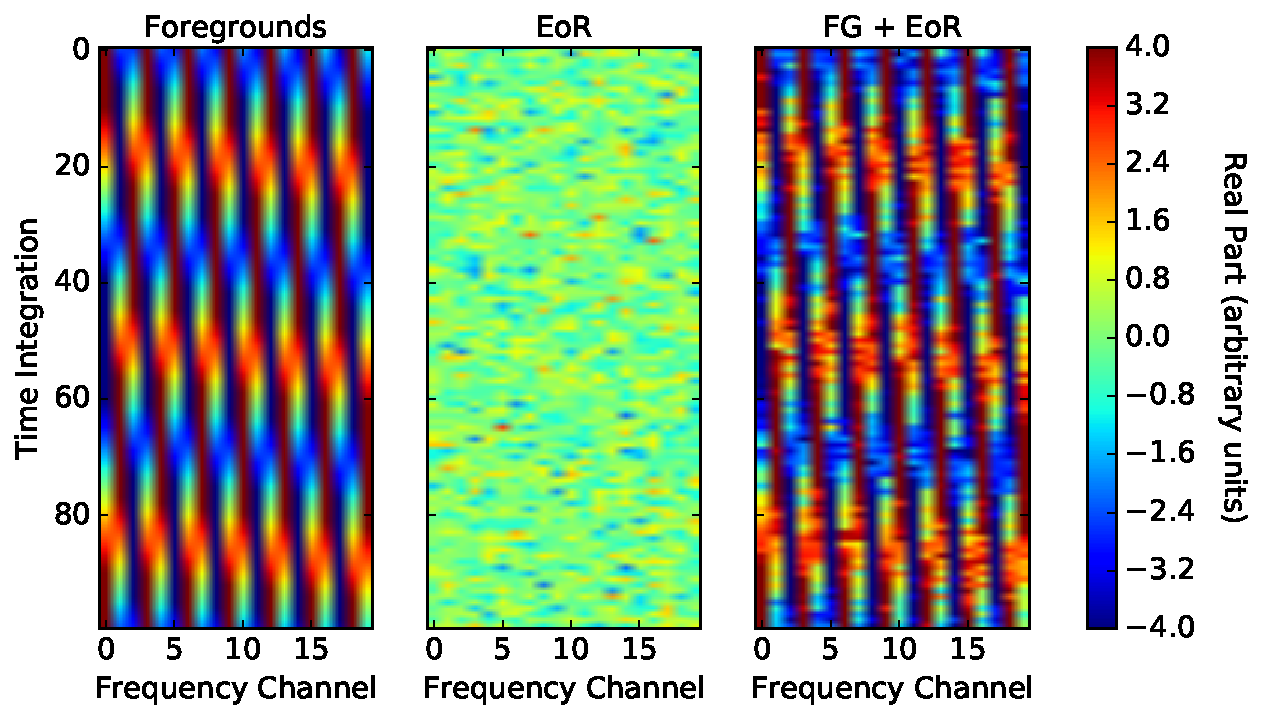
\includegraphics[trim={0cm 0cm 0cm 0cm},clip,width=0.7\textwidth]{plots/toy_sigloss1.pdf}
	\caption{Our toy model data set to which we apply different weighting schemes to in order to investigate signal loss. We model a mock foreground-only visibility with a sinusoid signal that varies smoothly in 
time and frequency. We model a mock visibility of an EoR signal as a random Gaussian signal. We add the two together to form $\textbf{x} = 
\textbf{x}_{\rm FG} + \textbf{x}_{\rm EoR}$. Real parts are shown here.}
	\label{fig:toy_sigloss1}
\end{figure}

%First, 
We compute the power spectrum of our toy model data set $\textbf{x}$ using Equations \eqref{eq:qhat} and \eqref{eq:phat}, with $\textbf{R} \equiv \widehat{\textbf{C}}^{-1}$.  Figure \ref{fig:toy_sigloss12} shows the estimated covariances of our toy model data sets along with the $\widehat{\textbf{C}}^{-1}$ weighted data. The foreground sinusoid is clearly visible in $\widehat{\textbf{C}}_{\rm FG}$.  The power spectrum result is shown in green in the left plot of Figure \ref{fig:toy_sigloss3}. Also plotted in the figure are the uniform-weighted ($\textbf{R} \equiv \textbf{I}$) power spectrum of the individual components $\textbf{x}_{\rm FG}$ (blue) and $\textbf{x}_{\rm EoR}$ (red). As shown, our $\widehat{\textbf{C}}^{-1}$ weighted result successfully suppresses foregrounds,
%For our toy model, the successful suppression of the foreground mode is 
demonstrated in Figure \ref{fig:toy_sigloss3} by the missing foreground peak in the weighted power spectrum estimate (green).  It is also evident that our result fails to recover the EoR signal --- it exhibits the correct shape, but the amplitude level is slightly low.  It is this behavior which we describe as signal loss.

\begin{figure}
	\centering
	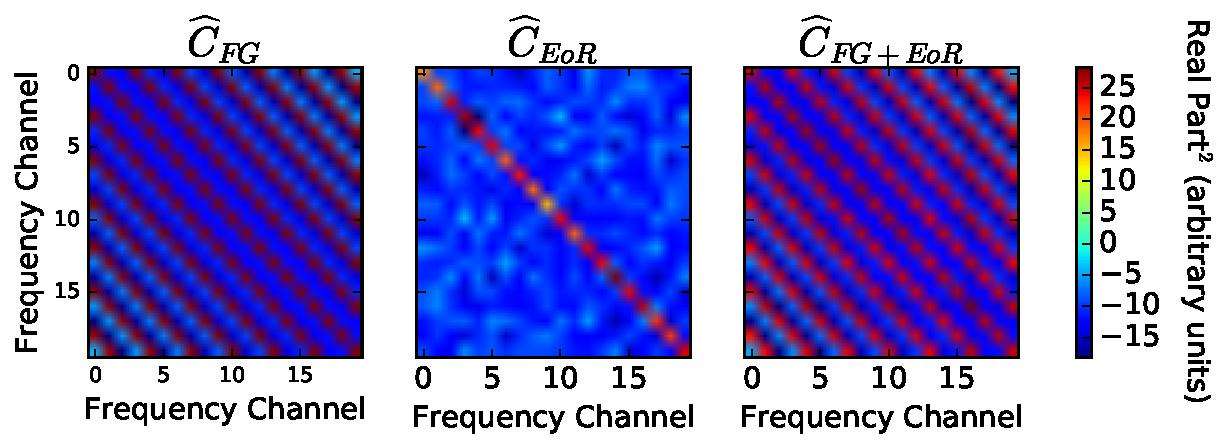
\includegraphics[trim={0cm 0cm 0cm 0cm},clip,width=0.7\textwidth]{plots/toy_sigloss12.pdf}
	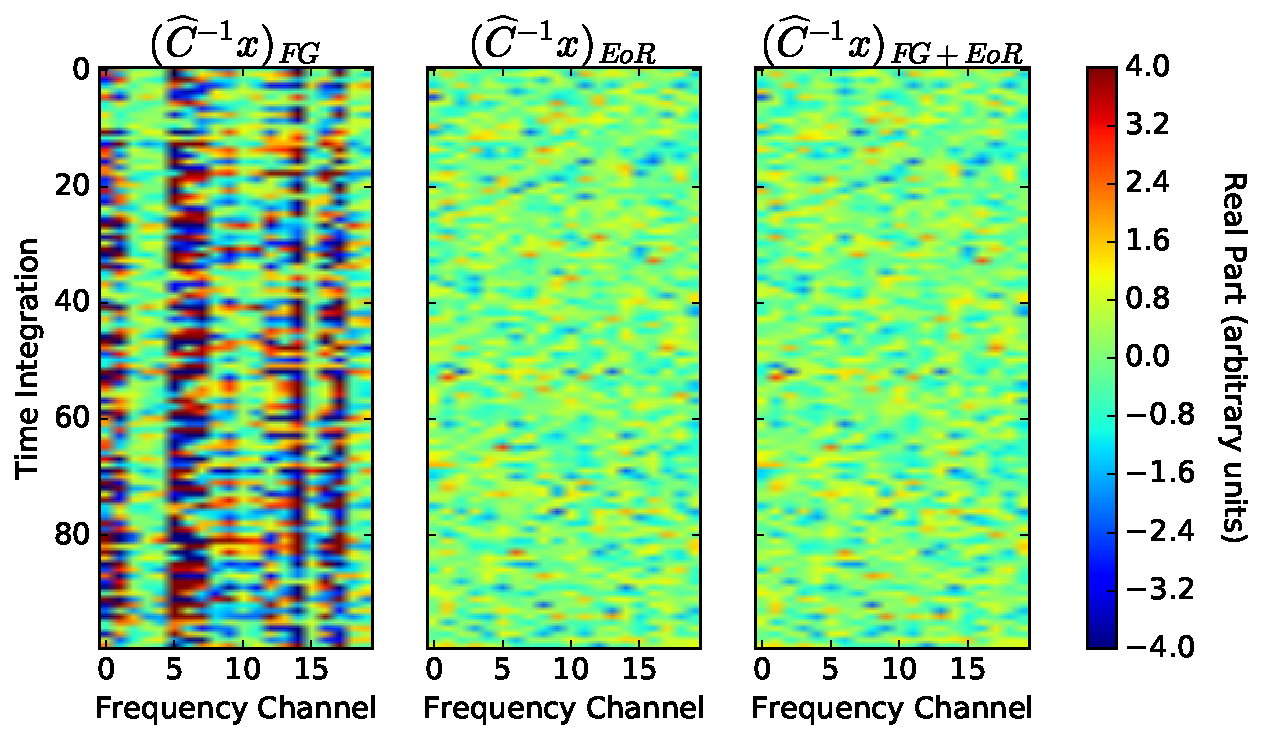
\includegraphics[trim={0cm 0cm 0cm 0cm},clip,width=0.7\textwidth]{plots/toy_sigloss13.pdf}
	\caption{The estimated covariance matrices (top row) and inverse covariance-weighted data (bottom row) for FG only (left), EoR only 
(middle), and FG + EoR (right). Real parts are shown here.}
	\label{fig:toy_sigloss12}
\end{figure}

\begin{figure*}
	\centering
	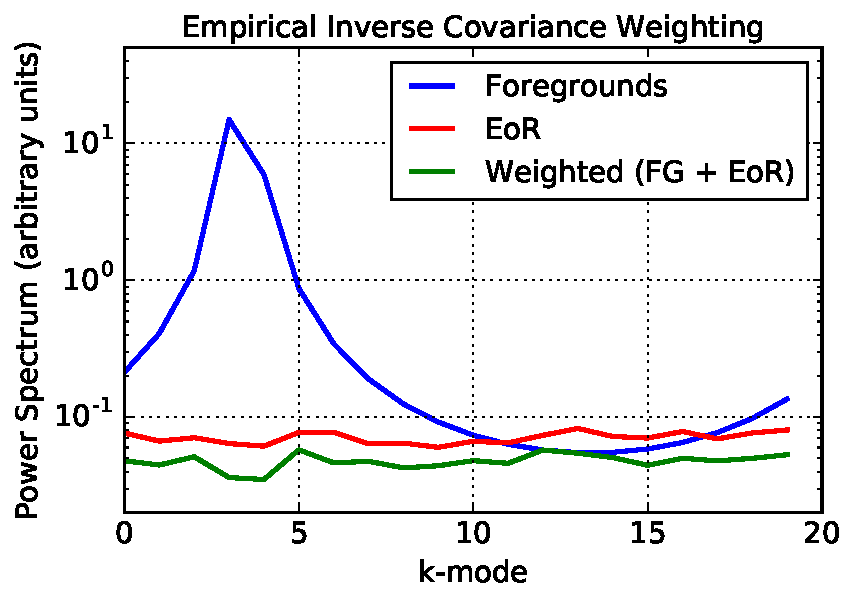
\includegraphics[trim={0cm 0cm 0cm 0cm},clip,height=0.33\textwidth]{plots/toy_sigloss3.pdf}
	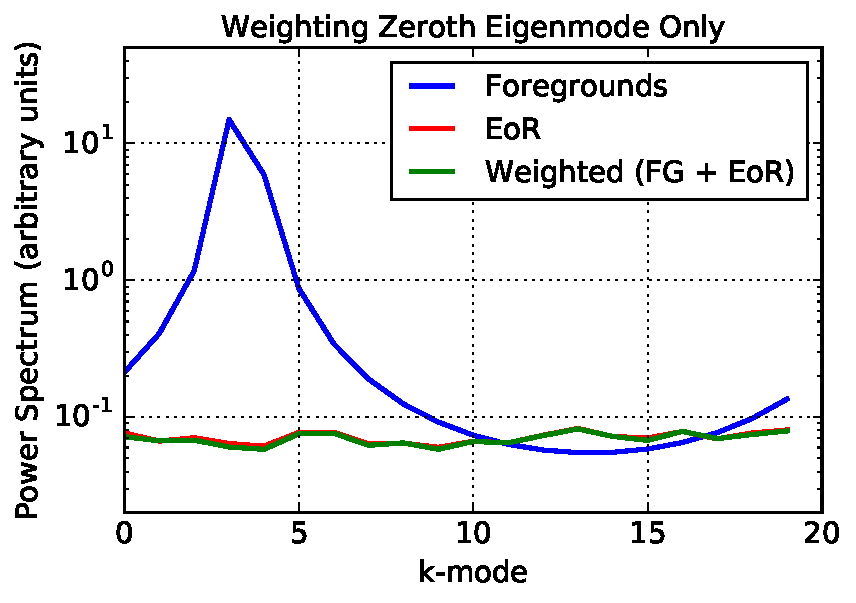
\includegraphics[trim={0cm 0cm 0cm 0cm},clip,height=0.33\textwidth]{plots/toy_sigloss4.pdf}
	\caption{Resulting power spectrum estimates for the toy model simulation described in Chapter \ref{sec:toymodel} --- foregrounds only (blue), EoR only (red), and the weighted FG + EoR data set (green). The power spectrum of the foregrounds peaks at a $k$-mode based on the frequency of the sinusoid used to create the mock FG signal. In the two panels, we compare using empirically estimated inverse covariance weighting where $\textbf{C}$ is derived from the data (left), and projecting out the zeroth eigenmode only (right). In the former case, signal loss arises from the coupling of the eigenmodes of $\widehat{\textbf{C}}$ to the data. 
% JEA - redundant
%For an empirically estimated $\widehat{\textbf{C}}$, 
%its eigenvalues differ from those of the true covariance, where 
%the coupling between EoR-dominated eigenmodes and the data can lead to loss.
%Hence, 
There is negligible signal loss when all eigenmodes besides the foreground one are no longer correlated with the data.
%assigning identical weights to all eigenmodes except the first, 
%constructing a covariance proportional to the identity and the outer product of the sinusoid eigenmode, since we are only down-weighting the FG-dominated mode in this case.
}
	\label{fig:toy_sigloss3}
\end{figure*}

As discussed in Chapter \ref{sec:QE}, this behavior is {\it not} expected in the case that we were to use a true $\textbf{C}^{-1}$ weighting.  Rather, we would obtain the behavior shown in the toy model in Chapter \ref{sec:icw_appendix}\footnote{Note that there the true covariance matrix is also the sum of a diagonal portion describing the signal and a single mode describing the contaminant (similar to Figure \ref{fig:toy_sigloss12}).}, with suppression of the foreground mode resulting in 
a nearly unbiased estimate of the power spectrum. The key difference is that since $\widehat{\textbf{C}}$ is estimated from the data, its eigenvectors and eigenvalues are strongly coupled to the particular data realization that was used to compute it, and this coupling leads to loss.

For the case of an eigenmode which can be safely assumed to be predominantly a foreground, its presence in the true covariance matrix will result in the desired suppression via a kind of projection; whether or not it is strongly correlated with the the actual data vector is irrelevant.  However, in the case of an empirically estimated covariance matrix, the eigenmodes of $\widehat{\textbf{C}}_{\rm EoR}$ will both be incorrect and can be correlated with the data. If these incorrect eigenmodes are not correlated with the data, it will lead to non-minimum variance estimates but will not produce the suppression of the power spectrum amplitude as seen in the left plot of Figure \ref{fig:toy_sigloss3}. As shown mathematically in Chapter \ref{sec:sigloss_appendix}, however, if $\widehat{\mathbf{C}}_{\rm EoR}$ $\textit{is}$ correlated with the data vector $\mathbf{x}$, there is a kind of projection of power in the {\it non}-foreground modes from the resulting power spectrum estimate, thus producing an estimate that is biased low.  In short, {\it if the covariance is computed from the data itself, it carries the risk of overfitting information in the data and introducing a multiplicative bias (per $k$) to estimates of the signal.} 

%For a toy model mathematical derivation of signal loss arising from a data-estimated covariance matrix, see Appendix \ref{sec:sigloss_appendix}. Here we will describe the origin of this signal loss intuitively.

%% JEA - I don't think the eigenspectrum really helps, but at some point we probably want to show it ...
%To begin to understand the lossy behavior of this result, we can closely study our estimated covariance eigenspectrum, shown in Figure \ref{fig:toy_sigloss2}. Since it is estimated from our data, its eigenspectrum differs from the eigenspectrum of the true covariance $\textbf{C}$, and this difference has important consequences on our result. 
%
%An eigenspectrum ranks the eigenvalues of a matrix from highest to lowest and can be thought of as a spectrum of weights that are given to each spectral mode in the data. In other words, the eigenvalues encode the strength of different shapes in the data set. The eigenspectrum of the identity matrix $\textbf{I}$ is flat (all $1$'s) because it gives equal weighting to all modes. In our application, covariance matrices tend to have sloped eigenspectra, meaning that modes are given different weights in QE power spectrum estimation. 
%% JEA - I think this is actually NOT true - see the toy model as an example.  The size of the eigenvalues isn't what determines that the undesired mode is downweighted and the others left alone.  I haven't computed the eigenvalues explicitly, but down-weighting of m occurs regardless of the relative size of s and u.
%The modes with the highest eigenvalues are down-weighted the most. 

%\begin{figure}
%	\centering
%	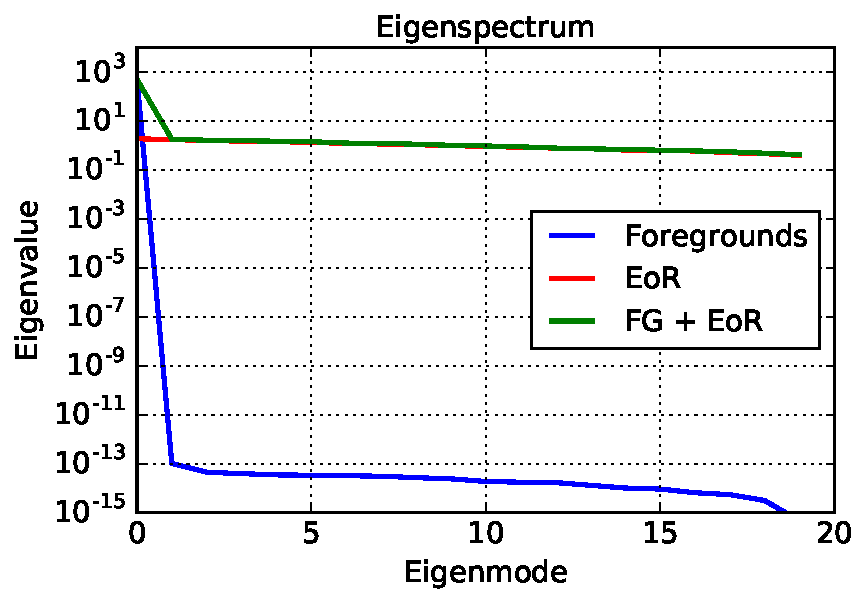
\includegraphics[trim={0cm 0cm 0cm 0cm},clip,width=\columnwidth]{plots/toy_sigloss2.pdf}
%	\caption{Eigenspectrum of $\widehat{\textbf{C}}_{\rm FG}$ (blue), $\widehat{\textbf{C}}_{\rm EoR}$ (red), and $\widehat{\textbf{C}}_{\rm FG+EoR}$ 
%(green). The eigenspectrum of $\widehat{\textbf{C}}_{\rm FG}$ peaks at the zeroth eigenmode, due to the presence of only one sinusoid. These empirically estimated covariance matrices have eigenspectra that are different from that of the true $\textbf{C}$. Specifically, these eigenmodes have the risk of being down-weighted more significantly than they should be because they are coupled to the data in a way that produces loss.}
%	\label{fig:toy_sigloss2}
%\end{figure}

%We show the {\it eigenspectrum} (the eigenvalues of the matrix in descending order) of this toy model in Figure \ref{fig:toy_sigloss2}.  In this case,
%For example, 
%the largest-valued eigenmode of $\widehat{\textbf{C}}$ (highest eigenvalue) describes the sinusoid foreground mode in the toy model (the peak in Figure \ref{fig:toy_sigloss3}). 
% 


%In general, the highest-valued eigenmodes of $\widehat{\textbf{C}}$ typically (but not always) describe bright foregrounds --- the most prominent shapes in a data set. For these FG-dominated modes, where foregrounds outshine the EoR signal, down-weighting is beneficial. In some sense, we desire signal loss in this regime, if by `signal' we mean `foregrounds.' In this case it is beneficial for these eigenmodes to be coupled to the data in a way that produces loss. 



%If the true covariance matrix $\textbf{C}$ of our data was known, then every single eigenvalue and eigenvector of $\textbf{C}$ would be 
%representative of real fluctuations in the data. However, when using an estimated $\widehat{\textbf{C}}$ that is derived from one 
%particular data realization, its eigenvalues and eigenvectors may differ from the truth. Said differently, shapes that may not exist (or exist rarely) in a true covariance may appear stronger in the estimated covariance. Hence, they will be down-weighted 
%more than they should be.



The danger of an empirically estimated covariance matrix comes mostly from not being able to describe the EoR-dominated eigenmodes of $\textbf{C}$ accurately, for which the EoR signal is brighter than foregrounds. In such a case, the coupling between these modes to the data realization leads to the overfitting and subtraction of the EoR signal. More specifically, the coupling between the estimated covariance and the data is anti-correlated in nature (which is explained in more detail in Chapters \ref{sec:sigloss_appendix} and \ref{sec:siglossmethod}), which leads to loss. Mis-estimating $\textbf{C}$ for EoR-dominated eigenmodes is therefore more harmful than for FG-dominated modes, and since the lowest-valued eigenmodes of an eigenspectrum are typically EoR-dominated, using this part of the spectrum for weighting is most dangerous.

Armed with this information,
%Using what we've learned about the eigenspectrum, 
we can tweak the covariance in a simple way to suppress foregrounds and yield minimal signal loss. Recall that our toy model foreground 
% JEA - modes need not be sinusoids; the point is that there is one outer product describing this in the covariance
%is a sinusoid, so it 
can be perfectly described by a single eigenmode. Using the full data set's (foreground plus EoR signal) empirical covariance, we can 
project out the zeroth eigenmode and 
%then flatten the rest of the spectrum to have eigenvalues of 1, thereby down-weighting the foreground-dominated mode more than the rest of the modes. Hence, we are changing the EoR-dominating part of the spectrum to be less coupled to the data, limiting the amount of overfitting that can happen for those modes (i.e., only allowing overfitting to occur for the first mode).
then take the remaining covariance to be the identity matrix.  
This decouples the covariance from the data for the EoR modes.  The resulting power spectrum estimate for this case is shown in the right plot of Figure \ref{fig:toy_sigloss3}. 
In this case we recover the EoR signal, demonstrating that if we can disentangle the foreground-dominated modes and EoR-dominated modes, we can suppress
% down-weight them 
foregrounds with negligible signal loss. 

Altering $\widehat{\textbf{C}}$ as such is one specific example of a regularization method for this toy model, in which we are changing $\widehat{\textbf{C}}$ in a way that reduces its coupling to the data realization. There are several other simple ways to regularize $\widehat{\textbf{C}}$, and we will discuss some in Chapter 
\ref{sec:otherweight}.

\subsection{Effect of Fringe-Rate Filtering}
\label{sec:toymodel_frf}

We have shown how signal loss can arise due to the coupling of EoR-dominated eigenmodes to the data. We will next show how this effect is exacerbated by reducing the total number of independent samples in a data set. 

A fringe-rate filter is an analysis technique designed to maximize sensitivity by integrating in time (\citealt{parsons_et_al2016}). Rather than a traditional box-car average in time, a time domain filter can be designed to up-weight temporal modes consistent with the sidereal motion on the sky, while down-weighting modes that are noise-like. 

Because fringe-rate filtering is analogous to averaging in time, it comes at the cost of reducing the total number of independent samples in the data. With fewer independent modes, it becomes more difficult for the empirical covariance to estimate the true covariance matrix of the fringe-rate filtered data. We can quantify this effect by evaluating a convergence metric $\varepsilon(\Chat)$ for the empirical covariance, which we define as

% JEA - Death to eigenspectra!
%The resulting eigenspectrum as compared to the green curve (FG + EoR) in Figure \ref{fig:toy_sigloss2} is shown in Figure \ref{fig:toy_sigloss15}. 

\begin{equation}
\label{eq:converge}
\varepsilon (\Chat) \equiv \sqrt{\frac{\sum_{ij} (\widehat{C}_{ij} - {C}_{ij})^2}{\sum_{ij} {C}_{ij}^2}},
\end{equation}
where $\C$ is the true covariance matrix. To compute this metric, we draw different numbers of realizations (different draws of Gaussian noise) of our toy model EoR measurement, $\textbf{x}_{\rm EoR}$, and take their ensemble average. We then compare this to the "true" covariance, which in our simulation is set to be the empirical covariance after a large number ($500$) of realizations. As shown in Figure \ref{fig:toy_sigloss16}, we perform this computation for a range of total independent ensemble realizations (horizontal axis) and number of independent samples in the data following time-averaging, or "fringe-rate filtering" (different colors). With more independent time samples (i.e., more realizations) in the data, one converges to the true fringe-rate filtered covariance more quickly. 

The situation here with using a finite number of time samples to estimate our covariance is analogous to a problem faced in galaxy surveys, where the non-linear covariance 
of the matter power spectrum is estimated using a large --- but finite --- number of expensive simulations. There, the limited 
number of independent simulations results in inaccuracies in estimated covariance matrices 
\citep{dodelson_schneider2013,taylor_joachimi_etal2014}, which in turn result in biases in the final parameter constraints 
\citep{hartlap_et_al2007}. In our case, the empirically estimated covariances are used for estimating the power spectrum, and 
as we discussed in the previous section (and will argue more thoroughly in Chapters \ref{sec:sigloss_appendix} and \ref{sec:siglossmethod}), couplings between these covariances and the data can lead to power spectrum estimates that are biased 
\emph{low}---which is precisely signal loss. In future work, it will be fruitful to investigate whether advanced techniques from the 
galaxy survey literature for estimating accurate covariance matrices can be successfully adapted for $21\,\textrm{cm}$ 
cosmology. These techniques include the imposition of sparsity priors \citep{padmanabhan_et_al2016}, the fitting of 
theoretically motivated parametric forms \citep{pearson_samushia2016}, covariance tapering \citep{paz_sanchez2015}, 
marginalization over the true covariance \citep{sellentin_heavens2016}, and shrinkage methods 
\citep{pope_szapudi2008,joachimi_2017}.

%Just as important as the eigenvalues are the eigenvectors of our empirical covariances. 
The overall convergence of the covariance is important, but also noteworthy is the fact that different eigenvectors converge to their true forms at different rates. This is illustrated by Figure \ref{fig:toy_sigloss17}, which shows the convergence of eigenvectors in an empirical estimate of a covariance matrix. For this particular toy model, we construct a covariance whose true form combines the same mock foreground from the previous toy models with an EoR component that is modeled as a diagonal matrix with eigenvalues spanning one order of magnitude (more specifically, we construct the EoR covariance as a diagonal matrix in the Fourier domain, where the signal is expected to be uncorrelated; its Fourier transform is then the true covariance of the EoR in the frequency domain, or $\textbf{C}_{\rm EoR}$). For different numbers of realizations, we draw random EoR signals that are consistent with $\textbf{C}_{\rm EoR}$, add them to the mock foreground data, and compute the combined empirical covariance by averaging over the realizations. The eigenvectors of this empirical covariance are then compared to the true eigenvectors $\textbf{v}$, where we use as a convergence metric $\varepsilon(\widehat{\textbf{v}})$, defined as:
\begin{equation}
\label{eq:converge_eig}
\varepsilon (\widehat{\textbf{v}}) \equiv \sqrt{\sum_{i}^{N_{f}}|\textbf{v}-\widehat{\textbf{v}}|_{i}^2},
\end{equation}
where $N_{f}$ is the number of frequencies ($20$) in the mock data. The eigenmode convergence curves in Figure \ref{fig:toy_sigloss17} are ranked ordered by eigenvalue, such that "Eigenmode \#0" illustrates the convergence of the eigenvector with the largest eigenvalue, "Eigenmode \#1" for the second largest eigenvalue, and so on. We see that the zeroth eigenmode --- the mode describing the foreground signal --- is quickest to converge.

Our numerical test reveals that the convergence rates of empirical eigenvectors is related to the sample variance in our empirical estimate. In general, computing an empirical covariance from a finite ensemble average means that the empirical eigenmodes have sample variances. Consider first a limiting case where all eigenvalues are equal. In such a scenario, any linear combination of eigenvectors is also an eigenvector, and thus there is no sensible way to define the convergence of eigenvectors. In our current test, aside from the zeroth mode, the eigenvalues have similar values but are not precisely equal. Hence, there is a well-defined set of eigenvectors to converge to. However, due to the sample variance of our empirical covariance estimate, there may be accidental degeneracies between modes, where some modes are mixing and swapping with others. Therefore, the steeper an eigenspectrum, the easier it is for the eigenmodes to decouple from each other and approach their true forms. A particularly drastic example of this can be seen in the behavior of mode $0$ (the foreground mode), whose eigenvalue differs enough from the others that it is able to converge reasonably quickly despite substantial sample variance in our empirical covariance estimate. To break degeneracies in the remaining modes, however, requires many more realizations.

While the connection between the rate of convergence of an empirical eigenvector with the sample variance of an eigenspectrum is interesting, it is also important to note that regardless of convergence rate, any mode that is coupled to the data is susceptible to signal loss. The true eigenvectors are not correlated with the data realizations; thus, if our empirical eigenvectors are converged fully, there will not be any signal loss. However, an unconverged eigenvector estimate will retain some memory of the data realizations used in its generation, leading to signal loss.

In the toy models throughout Chapter \ref{sec:SiglossOverview}, we exploit the fact that the strongest eigenmode (highest eigenvalue mode) is dominated by foregrounds in order to purposely incur signal loss for that mode. Even for the case of real PAPER data (Chapter \ref{c.PSA64}), we make the assumption that the strongest eigenmodes are likely the most contaminated by foregrounds. However, in general, foregrounds need not be restricted to the strongest eigenmodes, and as we have seen, it is really the degeneracies between modes that determines how quickly they converge, and hence how much signal loss can result.

%One sees that the highest-valued eigenmodes converge to their true eigenvectors more quickly. With only a small number of realizations, these empirically estimated modes already retain little correlation with the specific realizations of data that were used to form the empirical covariance. As we will see in the next section, using only these eigenmodes, which are less coupled to data realizations, minimizes signal loss. In contrast, the lower-valued eigenmodes retain more memory of the data realizations, which leads to correlations that induce signal loss. 
% JEA - this is redundant
%Said differently, a steep covariance eigenspectrum can be especially dangerous because the eigenmodes that converge the slowest are typically also EoR-dominated and are therefore susceptible to the most loss.  %\acl{Think about whether we need to do the Fourier space version as well.}

% JEA - death to eigenspectra!
%\begin{figure}
%	\centering
%	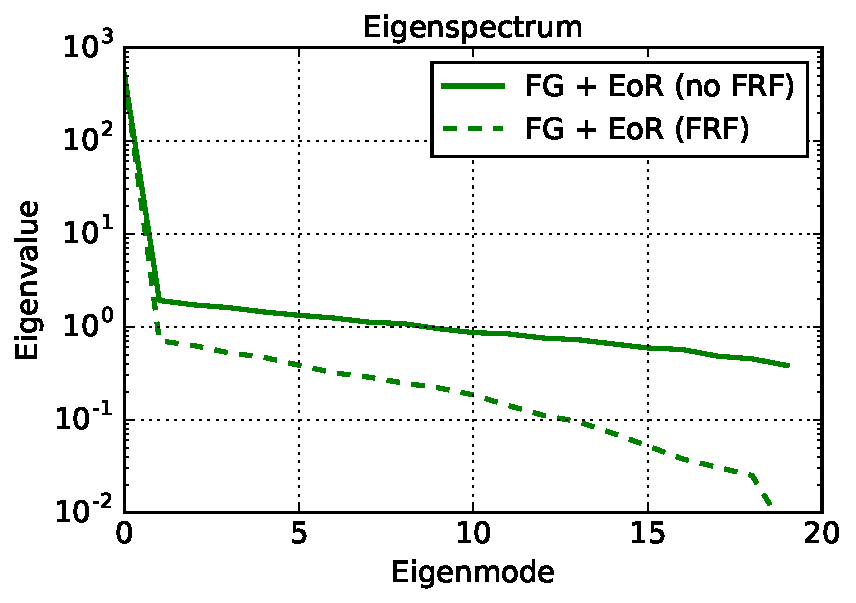
\includegraphics[trim={0cm 0cm 0cm 0cm},clip,height=0.31\textwidth]{plots/toy_sigloss15.pdf}
%	\caption{Eigenspectrum of $\widehat{\textbf{C}}_{\rm FG+EoR}$, in the case of no fringe-rate filtering (solid green) and with fringe-rate filtering (dashed green). The dashed, steep eigenspectrum has a greater risk of signal loss because its lowest-valued eigenmodes are both more strongly coupled to the data (than those of the solid eigenspectrum) and, in this example, are also EoR-dominated.}
%	\label{fig:toy_sigloss15}
%\end{figure}

\begin{figure}
	\centering
	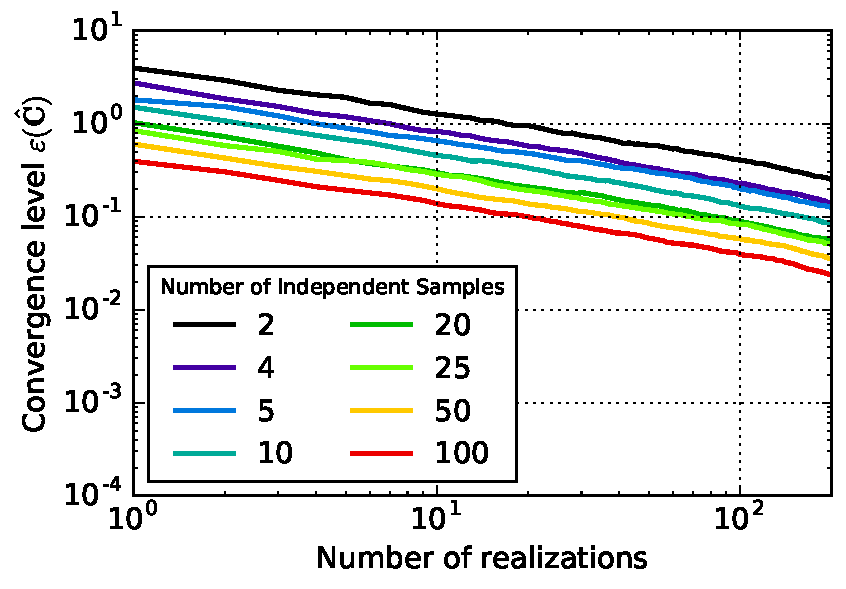
\includegraphics[width=0.55\textwidth]{plots/toy_sigloss16.pdf}
	\caption{The convergence level, as defined by Equation \eqref{eq:converge}, of empirically estimated covariances of mock EoR signals with different numbers of independent samples. In red, the mock EoR signal is comprised entirely of independent samples (100 of them). Subsequent colors show time-averaged signals. As the number of realizations increases, we see that the empirical covariances approach the true covariances. With more independent samples, the quicker an empirical covariance converges (i.e., the quicker it decouples from the data), and the less signal loss we would expect to result.}
	\label{fig:toy_sigloss16}
\end{figure}

\begin{figure}
	\centering
	\includegraphics[width=0.7\textwidth]{plots/toy_sigloss17.pdf}
	\caption{The convergence level, as defined by Equation \eqref{eq:converge_eig}, of empirically estimated eigenvectors for different numbers of mock data realizations. The colors span from the 0th eigenmode (has the highest eigenvalue) to the 19th eigenmode (has the lowest eigenvalue), where they are ordered by eigenvalue in descending order. This figure shows that the zeroth eigenmode converges the quickest, implying that eigenvectors with eigenvalues that are substantially different than the rest (the FG-dominated mode has a much higher eigenvalue than the EoR modes) are able to converge to the true eigenvectors the quickest. On the other hand, eigenmodes $1$-$19$ have similar eigenvalues and are slower to converge because of degeneracies between them.}
	\label{fig:toy_sigloss17}
\end{figure}

\begin{figure}
	\centering
	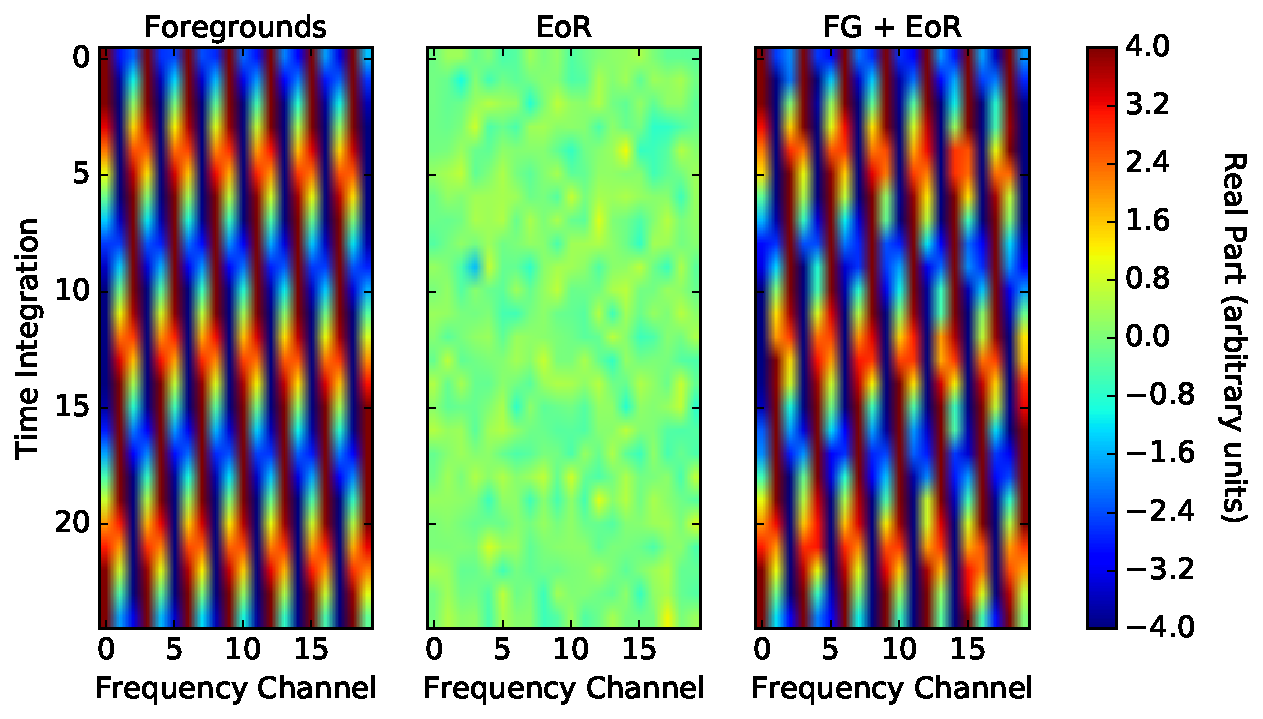
\includegraphics[width=0.7\textwidth]{plots/toy_sigloss5.pdf}
	\caption{Our "fringe-rate filtered" (time-averaged) toy model data set. We average every four samples together, 
yielding $25$ independent samples in time. Real parts are shown here.}
	\label{fig:toy_sigloss5}
\end{figure}


With Figures \ref{fig:toy_sigloss16} and \ref{fig:toy_sigloss17} establishing the connection between convergence rates (of empirical covariances and eigenvectors) and number of realizations, we now turn back to our original toy model used in Chapter \ref{sec:toymodel}, which is comprised of a mock foreground and mock EoR signal. We mimic a fringe-rate filter by averaging every four time integrations of our toy model data set together, yielding $25$ independent samples in time (Figure \ref{fig:toy_sigloss5}). We choose these numbers so that the total number of independent samples is similar to the number of frequency channels --- hence our matrices will be full rank. We use this "fringe-rate filtered" mock data for the remainder of Chapter \ref{sec:SiglossOverview}.
%\footnote{If instead we average every $20$ samples together, yielding only $5$ independent samples in time, we are left with a rank deficient covariance matrix. In this case... \cc{fill in}}

The power spectrum results for this model are shown in Figure \ref{fig:toy_sigloss7}, and as 
expected there is a much larger amount of signal loss for this time-averaged data set since we do a worse job estimating the true covariance. In addition, as a result of having fewer independent samples, we obtain an estimate with more scatter. This is evident by noticing that the 
green curve in Figure \ref{fig:toy_sigloss7} fails to trace the shape of the uniform-weighted EoR power spectrum (red). 

Using our toy model, we have seen that a sensitivity-driven analysis technique like fringe-rate filtering has trade-offs of signal 
loss and noisier estimates when using data-estimated covariance matrices. Longer integrations increase sensitivity but reduce 
the number of independent samples, resulting in 
eigenmodes correlated with the data
% JEA - it's not that they are wrong, but that they are correlated
%poorly characterized, steep eigenspectra 
that can overfit signal greatly. We 
note that a fringe-rate filter does have a range of benefits, many described in \citet{parsons_et_al2016}, so it can still be 
advantageous to use one despite the trade-offs.

\begin{figure}
	\centering
	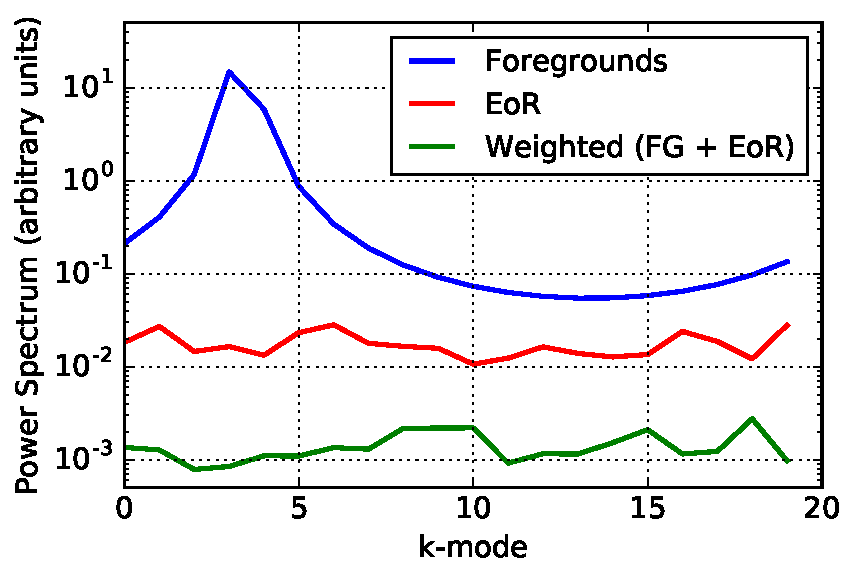
\includegraphics[trim={0cm 0cm 0cm 0cm},clip,width=0.7\textwidth]{plots/toy_sigloss7.pdf}
	\caption{Resulting power spectrum estimate for the "fringe-rate filtered" (time-averaged) toy model simulation --- foregrounds only (blue), 
EoR only (red), and the weighted FG + EoR data set (green). We use empirically estimated inverse covariance weighting where $\textbf{C}$ is 
computed from the data. There is a larger amount of signal loss than for the non-averaged data, a consequence of weighting by eigenmodes that are more strongly coupled to the data due to there being fewer independent modes in the data.}
	\label{fig:toy_sigloss7}
\end{figure}

\subsection{Other Weighting Options}
\label{sec:otherweight}

In Chapter \ref{sec:toymodel} we showed one example of how altering $\widehat{\textbf{C}}$ can 
make the difference between nearly zero and some signal loss. We will now use our toy model to describe several other ways to tailor $\widehat{\textbf{C}}$ 
in order to minimize signal loss. We choose four independent regularization methods to highlight in this section, which have 
been chosen due to their simplicity in implementation and straightforward interpretations. We illustrate the resulting power 
spectra for the different cases in Figure \ref{fig:toy_sigloss8}.
% and \ref{fig:toy_sigloss14}. 
These examples are not meant to be taken as suggested analysis methods but rather as illustrative cases. 

As a first test, we model the covariance matrix of EoR as a proof of concept that if perfect models are known, signal loss can be 
avoided. We know that our simulated EoR signal should have a covariance matrix that mimics the identity matrix, with its 
variance encoded along the diagonal. We model $\textbf{C}_{\rm EoR}$ as such (i.e., the identity), instead of computing it based on $\textbf{x}
_{\rm EoR}$ itself. Next, we add $\textbf{C}_{\rm EoR} + \widehat{\textbf{C}}_{\rm FG}$ (where $\widehat{\textbf{C}}_{\rm FG} = \langle\textbf{x}_{\rm FG}
\textbf{x}_{\rm FG}^{\dagger}\rangle_{t}$) to obtain a final $\widehat{\textbf{C}}_{\rm reg}$ (regularized empirical covariance matrix) to use in weighting. In Figure \ref{fig:toy_sigloss8} (upper 
left), we see that there is negligible signal loss. This is because by modeling $\textbf{C}_{\rm EoR}$, we avoid overfitting EoR fluctuations in the data that our model doesn't know about (but, an empirically derived $\widehat{\textbf{C}}_{\rm EoR}$ would know about the fluctuations). 
%This is also shown by comparing the (steeper) green and (flatter) red curves in Figure \ref{fig:toy_sigloss14}. 
In practice such a weighting option is not feasible, as it is difficult to model $\textbf{C}_{\rm EoR}$, and $\widehat{\textbf{C}}_{\rm FG}$ is unknown because we do not know how to separate out the foregrounds from the EoR in our data.

\begin{figure*}
	\centering
	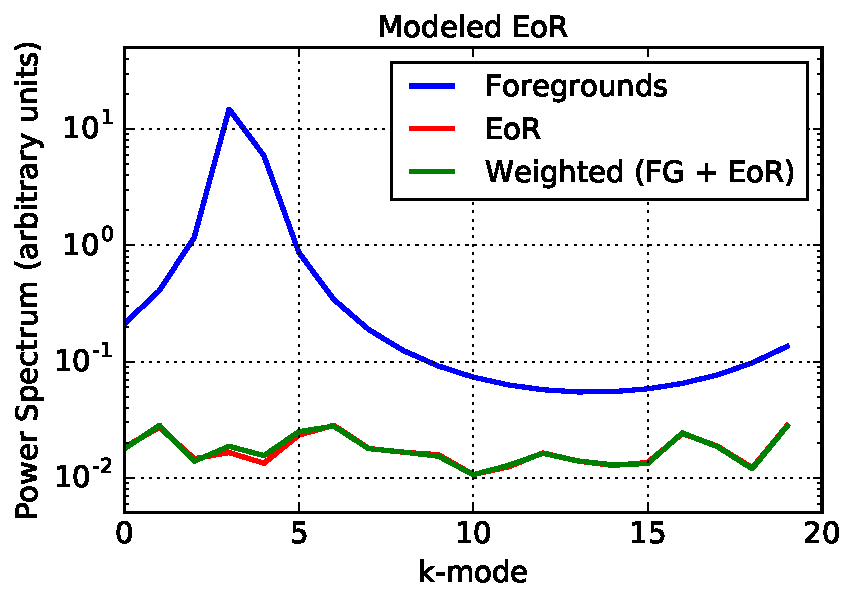
\includegraphics[trim={0cm 0cm 0cm 0cm},clip,height=0.33\textwidth]{plots/toy_sigloss10.pdf}
	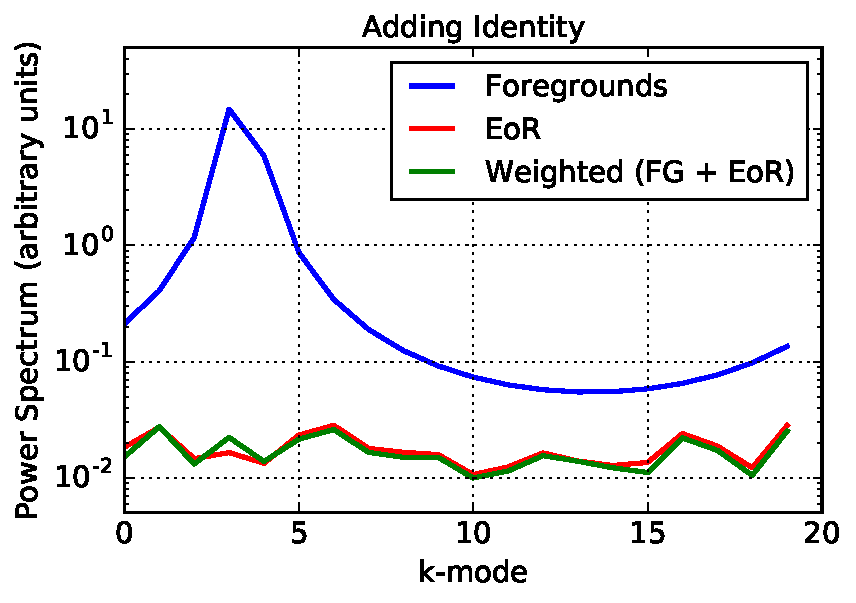
\includegraphics[trim={0cm 0cm 0cm 0cm},clip,height=0.33\textwidth]{plots/toy_sigloss8.pdf}
	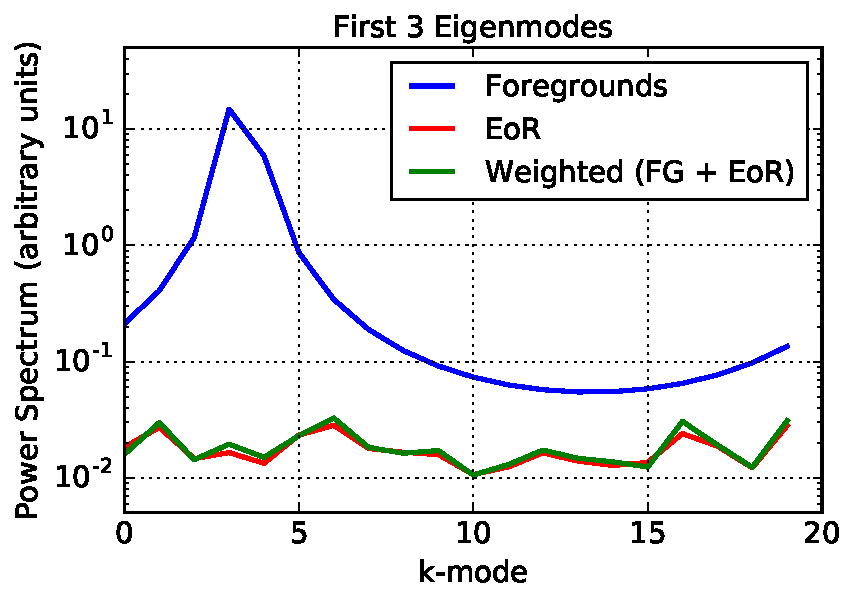
\includegraphics[trim={0cm 0cm 0cm 0cm},clip,height=0.33\textwidth]{plots/toy_sigloss9.pdf}
	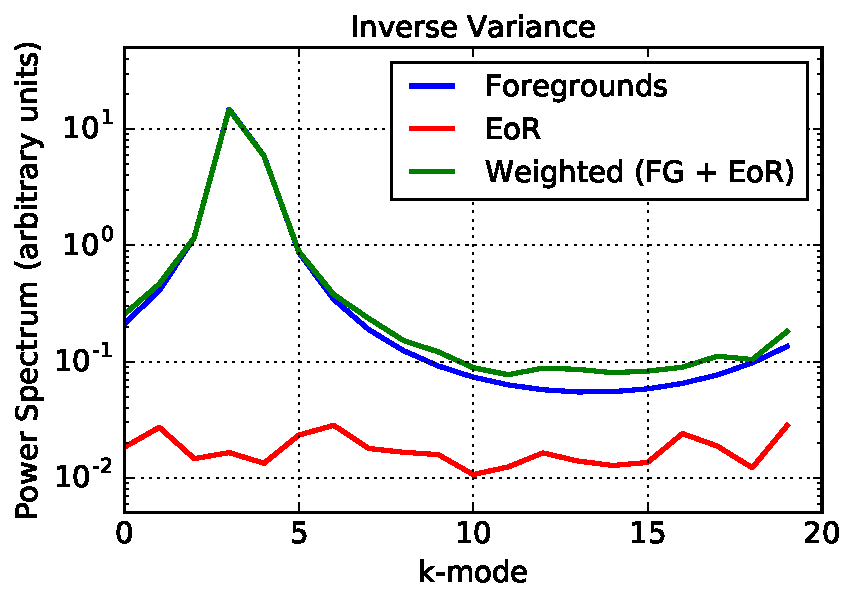
\includegraphics[trim={0cm 0cm 0cm 0cm},clip,height=0.33\textwidth]{plots/toy_sigloss11.pdf}
	\caption{Resulting power spectra estimates for our "fringe-rate filtered" (time-averaged) toy model simulation --- foregrounds only (blue), EoR only (red), and the weighted FG + EoR data set (green). We show four alternate weighting options that each minimize signal loss, including modeling the covariance matrix of EoR (upper left), regularizing $\widehat{\textbf{C}}$ by adding an identity matrix to it (upper right), using only the first three eigenmodes of $\widehat{\textbf{C}}$ (lower left), and keeping only the diagonal elements of $\widehat{\textbf{C}}$ (lower right). The first case (upper left) is not feasible in practice since we do not know $\textbf{C}_{\rm FG}$ and $\textbf{C}_{\rm EoR}$ like we do in the toy model.}
	\label{fig:toy_sigloss8}
\end{figure*}

%\begin{figure}
%	\centering
%	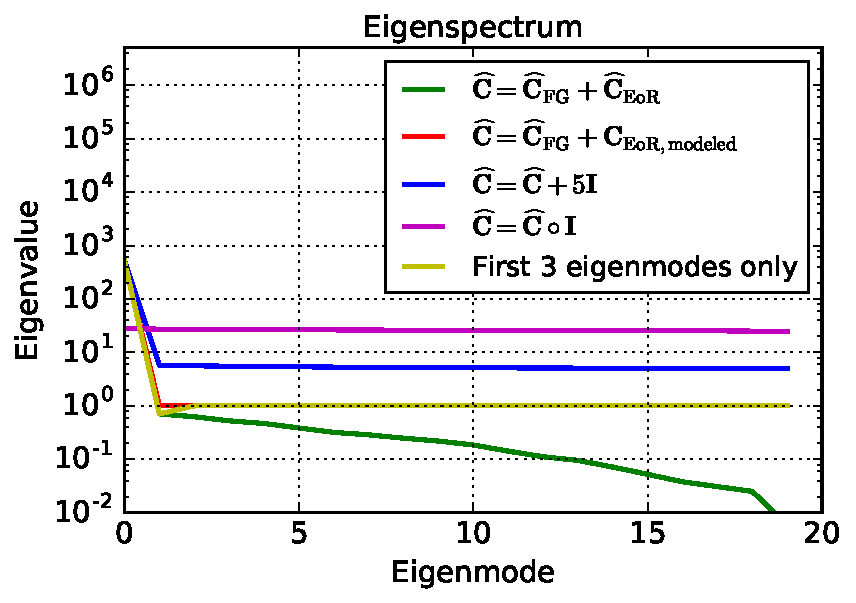
\includegraphics[trim={0cm 0cm 0cm 0cm},clip,width=\columnwidth]{plots/toy_sigloss14.pdf}
%	\caption{We compare the eigenspectrum of an empirically calculated $\widehat{\textbf{C}}$ (green) to that of four alternate 
%weighting options, including modeling the covariance matrix of EoR (red), regularizing $\widehat{\textbf{C}}$ by adding an identity 
%matrix to it (blue), using only the first three eigenmodes of $\widehat{\textbf{C}}$ (yellow), and multiplying an identity matrix with $
%\widehat{\textbf{C}}$ (magenta). All eigenspectra (except the green) are relatively flat and don't exhibit signal loss. All were 
%computed for the `fringe-rate filtered' (time-averaged) toy model case presented in Chapter \ref{sec:toymodel_frf}.}
%	\label{fig:toy_sigloss14}
%\end{figure}
%
The second panel (top right) in Figure \ref{fig:toy_sigloss8} uses a regularization method of setting $\widehat{\textbf{C}}_{\rm reg} \equiv 
\widehat{\textbf{C}} + \gamma\textbf{I}$, where $\gamma = 5$ (an arbitrary strength 
of $\textbf{I}$ for the purpose of this toy model). By adding the identity matrix, element-wise, we are weighting the diagonal 
elements of the estimated covariance matrix more heavily than those off-diagonal. Since the identity component does not know anything about the data realization, it alters the covariance to be less coupled to the data and there is no loss. %Although there is negligible signal loss using this regularization, the small green peak at the fourth $k$-mode represents residual foregrounds that still exist since the shapes encoded in the off-diagonal frequency correlations of the covariance matrix were deemed not as prominent as the diagonal elements using this weighting scheme. 

The third panel (bottom left) in Figure \ref{fig:toy_sigloss8} minimizes signal loss by only using the first three eigenmodes of the estimated covariance. Recalling that our toy model foregrounds can be described entirely by the zeroth eigenmode, this 
method intentionally projects out the highest-valued modes only by replacing all but the three highest weights in the 
eigenspectrum with $1$'s (equal weights). Again, avoiding the overfitting of EoR-dominated modes which are coupled to the data results in negligible signal loss. While this case is illuminating for the toy model, in practice it is not obvious which eigenmodes are foreground or EoR dominated (and they could be mixed as well), so determining which subset of modes to down-weight is not trivial. We experiment with this idea using PAPER data in Chapter \ref{sec:Weight}.

The last regularization scheme we are highlighting here is setting $\widehat{\textbf{C}}_{\rm reg} \equiv \widehat{\textbf{C}} \circ \textbf{I}$ (element-wise multiplication), or inverse variance weighting (i.e., keeping only the diagonal elements of $\widehat{\textbf{C}}$). In the bottom right 
panel of Figure \ref{fig:toy_sigloss8}, we see that this method does not down-weight the foregrounds at all --- this regularization altered $\widehat{\textbf{C}}$ in a way where it is no longer coupled to \textit{any} of the empirically estimated eigenmodes, including the FG-dominated one. To understand this, we recall that our foregrounds are spread out in frequency and therefore have non-negligible frequency-frequency correlations. Multiplying by 
the identity matrix, element-wise, results in a diagonal matrix, meaning we do not have any correlation information. Because of this, we do a poor job 
suppressing the foreground. But because we decoupled the whole eigenspectrum from the data, we also avoid signal loss. Although this method did not successfully recover the EoR signal for this particular simulation, it is important that we show that there 
are many options for estimating a covariance matrix, and some may down-weight certain eigenmodes more effectively than others based on the spectral nature 
of the components in a data set. 
%One may imagine a situation where a particular systematic is contained to an isolated 
%frequency (such as radio frequency interference or crosstalk). In such a case, preserving only the diagonal elements of $
%\widehat{\textbf{C}}$ would be an effective way of removing this contamination. 

In summary, we have shown how signal loss is caused by weighting a data set by itself, and in particular how estimated covariances can overfit EoR modes when they are coupled to data and not converged to their true forms. We have also seen that there are trade-offs between a chosen weighting method, its foreground-removal effectiveness, the number of independent samples in a data set, and the amount of resulting signal loss. 

\section{Signal Loss Mathematical Framework}
\label{sec:SiglossMath}

In Chapter \ref{sec:QE}, we argued that the optimal quadratic estimator method has the effect of projecting out foreground modes that have a different covariance structure than the EoR signal. And in Chapter \ref{sec:toymodel}, we saw that \textit{empirical} inverse covariance weighting can lead to loss via a multiplicative bias to estimates of the signal. To support these arguments, we now present two mathematical frameworks in which we use toy models in order to illustrate these conclusions analytically. 

\subsection{A Toy Model for Inverse Covariance Weighting}
\label{sec:icw_appendix}

%AAAXXX

In this section, we focus on the optimal quadratic estimator, Equation \eqref{eq:OQE}, and mathematically illustrate its role in estimating the power spectrum of EoR. While there exists detailed literature about quadratic estimators in general (e.g., \citealt{liu_tegmark2011}; \citealt{trott_et_al2012}; \citealt{liu_et_al2014b}; \citealt{dillon_et_al2014}), here we focus on two simple cases in order to outline one situation where the estimator successfully suppresses contamination and one where it does not. By describing these two cases, we hope to clarify and motivate the desire to use OQE while also understanding its limitations.

In our toy model, we specifically choose models where the data covariance is diagonal, as indeed we expect the EoR signal to be. We assume we have $N$ data points $\Delta_i$ which are the sum of a desired signal $\sigma_i$ and an undesired contaminant $\upsilon_i$
\begin{equation}
\Delta_i = \sigma_i + \upsilon_i
\end{equation}
with 
\begin{equation}
\langle \sigma_i \rangle = 0; \; \langle \sigma^2_i \rangle = s; \; {\rm and}~\langle \bm{\sigma \sigma}^T \rangle = s \mathbf{I}_{N \times N} \equiv \mathbf{S},
\end{equation}
where we wish to estimate $s$.  The contaminant in this first case has a similar structure (as the EoR) for its covariance, and is assumed uncorrelated with the signal
\begin{equation}
\label{eq:IdealToyModelCovariance}
\langle \upsilon_i \rangle = 0; \; 
\langle \upsilon^2_i \rangle = u; \; 
\langle \bm{\upsilon \upsilon}^T \rangle = u \mathbf{I}_{N \times N} \equiv \mathbf{U}; {\rm and}~ 
\langle \sigma_i \upsilon_j \rangle = 0.
\end{equation}
With the covariance matrix given by $\C = \mathbf{S} + \mathbf{U}$, the estimator for $s$ using only the quadratic part of Equation \ref{eq:OQE} is
\begin{equation}
\label{eq:IdealToyModelEstimator}
\hat{s} = \frac{ \bm{\Delta^T \Delta}}{N} 
\end{equation}
and its expectation is
\begin{equation}
\langle \hat{s} \rangle = s + u.
\end{equation}
Thus, {\it when the covariance structure of the contaminant is identical to the signal} ($\PDeriv{\mathbf{S}}{s} = \PDeriv{\mathbf{U}}{u} =  \PDeriv{\C}{s}$), the information available to the quadratic portion of the estimator to distinguish between the two is degenerate, and knowledge only of $\C$ and $\PDeriv{\C}{s}$ is inadequate.  In order to obtain an unbiased estimate of $s$, one must also use knowledge of $\mathbf{U}$.  Indeed, computing the linear bias from Equation \eqref{eq:OQELinear}, one finds $b = u$.   

Now consider a case, chosen to be very similar to the toy model in \ref{sec:toymodel},  in which the data again have an additive contaminant, now given by
\begin{equation}
\Delta_i = \sigma_i + \upsilon m_i
\end{equation}
where the properties of $\sigma_i$ are as before, but now $\upsilon$ is a random variable and $m_i$ is a fixed function of $i$ with
\begin{equation}
\langle \upsilon \rangle = 0; \;
\langle \upsilon^2 \rangle = u; \; 
 \langle \bm{\upsilon \upsilon}^T \rangle = u \mathbf{m m}^T \equiv \mathbf{U}; \;
 \mathbf{m}^T \mathbf{m} = 1; \; {\rm and}~ 
\langle \sigma_i \upsilon \rangle = 0.
\end{equation}
Here $\mathbf{m}$ represents a mode which is correlated across many data points (i.e., we are assuming $\mathbf{U}$ need {\it not} be diagonal), with amplitude given by  $\upsilon$.  The normalization of $\mathbf{m}$ is a matter of convention, and can be absorbed in the variance $u$; the choice above will be convenient for understanding the limiting case $u \gg s$.

We can calculate the quadratic portion of the estimator explicitly by using the Sherman-Morrison identity to invert the covariance matrix.  Defining
\begin{equation}
\xi \equiv \frac{u/s}{1+u/s},
\end{equation} 
we have
\begin{equation}
\invC  =   \frac{1}{s} \left(\I - \xi \mathbf{m m}^T \right)
\end{equation}
and
\begin{equation}
\hat{s} = 
%\half {\F}^{-1} \left(\bm \Delta^T \invC \PDeriv{\C}{s}  \invC \bm \Delta \right) = 
\frac{ \bm \Delta^T  (\I +  (\xi^2 - 2 \xi)  \mathbf{m m}^T)  \bm \Delta}{N + \xi^2 - 2 \xi} 
\end{equation}
with expectation
\begin{equation}
\langle \hat{s} \rangle = 
s + \frac{1 - 2 \xi + \xi^2}{N + - 2 \xi + \xi^2} u. 
\end{equation}
It is worth observing immediately that there is no multiplicative bias on $s$, and that the additive bias is strictly $< u/N$.

An instructive limit is $u \gg s$, $\xi \to 1$, in which case the virtue of weighting by $\invC$ becomes clearer, as it becomes
\begin{equation}
\invC  = \frac{1}{s} \left(\I - \mathbf{m m}^T \right)
\end{equation}
where $\I - \mathbf{m m}^T$ is the projection operator, projecting out $\mathbf{m}$ from any vector it acts on, and further, the linear bias tends to 0 as $\xi \to 1$ (i.e., the projection is "perfect'' and not "undone'' by the Fisher matrix normalization).

This is the ideal case for the inverse covariance weighting performed in the PAPER analysis, where removal of contamination with a known covariance can be suppressed by a kind of projection of the offending modes.  But even in this case, it is worth pointing out that the estimator still has a linear bias for finite $u$.  We have also assumed that the contaminating mode $\mathbf{m}$ is known perfectly; the next section takes up the case where the modes are estimated from the data.

\color{black}

%\appendix
\subsection{A Toy Model for Signal Loss}
\label{sec:sigloss_appendix}

In this section, we examine a toy model for signal loss. Our goal is to derive an analytic formula for power spectrum signal loss. While this model does not apply generally to all the scenarios presented in this work, it provides some analytic intuition for how the coupling between data and an empirical covariance can result in signal loss.

The minimum-variance quadratic estimator $\widehat{P}^\alpha$ for the $\alpha$th bandpower of the power spectrum is given by 
\begin{equation}
\widehat{P}^\alpha = \frac{1} {2 \F^{\alpha \alpha} }\x^t \C^{-1} \Q^{\alpha} \C^{-1} \x,
\end{equation}
where
\begin{equation}
F^{\alpha \alpha} \equiv \frac{1}{2} \textrm{tr} \left( \C^{-1} \Q^\alpha \C^{-1} \Q^\alpha \right)
\end{equation}
is the $\alpha$th diagonal element of the Fisher matrix. For this section only, with no loss of generality, we assume that the data $\textbf{x}$ are real. We also assume for simplicity that $\mathbf{x}$ is the data from a single instant in time, so that it is of length $N_f$, where $N_f$ is the number of frequency channels.

In our case, we do not have \emph{a priori} knowledge of the covariance matrix. Thus, we deviate from the true minimum-variance quadratic estimator and replace $\C$ with $\Chat$, its data-derived approximation. Our estimator then becomes
\begin{equation}
\label{eq:phatloss}
\widehat{P}^\alpha_\textrm{loss} = \frac{1} {2 \widehat{\F}^{\alpha \alpha} }\x^t \Chat^{-1} \Q^{\alpha} \Chat^{-1} \x,
\end{equation}
where
\begin{equation}
\widehat{F}^{\alpha \alpha} \equiv \frac{1}{2} \textrm{tr} \left( \Chat^{-1} \Q^\alpha \Chat^{-1} \Q^\alpha \right),
\end{equation}
with the label "loss" to foreshadow the fact that this will be an estimator with signal loss (i.e., a multiplicative bias of less than unity). We will now provide an explicit demonstration of this by modeling the estimated covariance as
\begin{equation}
\label{eq:ChatDef}
\Chat = (1-\eta) \C + \eta \x \x^t,
\end{equation}
where $\eta$ is a parameter quantifying our success at estimating the true covariance matrix. If $\eta = 0$, our covariance estimate has perfectly modeled the true covariance and $\Chat = \C$. On the other hand, if $\eta =1$, then our covariance estimate is based purely on the one realization of the covariance that is our actual data, and we would expect a high level of overfitting and signal loss.

Our strategy for computing the signal loss will be to insert Equation \eqref{eq:ChatDef} into Equation \eqref{eq:phatloss} and to express the resulting estimator $\widehat{P}^\alpha_\textrm{loss}$ in terms of $\widehat{P}^\alpha$. We begin by expressing $\Chat^{-1}$ in terms of $\C^{-1}$ using the Woodbury identity so that
\begin{equation}
\Chat^{-1} = \frac{\C^{-1}}{1-\eta} \left[ \I - \frac{\eta \x \x^t \C^{-1}}{1+ \eta (g-1)}\right],
\end{equation}
where we have defined $g \equiv \x^t \C^{-1} \x$. Inserting this into our Fisher estimate we have
\begin{equation}
\widehat{F}^{\alpha \alpha} = \frac{F^{\alpha \alpha}}{(1-\eta)^2} \left[ 1 -\frac{\eta }{1+ \eta (g-1)} \frac{h^{\alpha \alpha}}{F^{\alpha \alpha}} + \frac{1}{2} \left( \frac{\eta }{1+ \eta (g-1)} \right)^2 \frac{(h^{\alpha})^2}{F^{\alpha \alpha}}\right],
\end{equation}
where $h^\alpha \equiv \x^t \C^{-1} \Q^\alpha \C^{-1} \x $ and $h^{\alpha \alpha} \equiv \x^t \C^{-1} \Q^\alpha \C^{-1} \Q^\alpha \C^{-1}\x $. Note that $g$, $h^\alpha$, and $h^{\alpha \alpha}$ are all random variables, since they depend on $\x$. Inserting these expressions into our estimator gives
\begin{equation}
\label{eq:phatlossexpanded}
\widehat{P}^\alpha_\textrm{loss} = \frac{1}{2} \frac{h^\alpha}{F^{\alpha \alpha}} \left[ 1 - \frac{\eta g}{1+ \eta (g-1)}\right]^2  \left[ 1 -\frac{\eta }{1+ \eta (g-1)} \frac{h^{\alpha \alpha}}{F^{\alpha \alpha}} + \frac{1}{2} \left( \frac{\eta }{1+ \eta (g-1)} \right)^2 \frac{(h^\alpha)^2}{F^{\alpha \alpha}}\right]^{-1}.
\end{equation}
Both for the purposes of analytical tractability and to provide intuition, we expand this expression to leading 
order in $\eta$. This approximates the limiting case where the covariance $\Chat$ is close to the ideal and the 
lossy covariance is a small perturbation.  The result is
\begin{equation}
\widehat{P}^\alpha_\textrm{loss} \approx \frac{1}{2} \frac{h^\alpha}{F^{\alpha \alpha}} \left[ 1 - \eta \left( g - \frac{h^{\alpha \alpha}}{F^{\alpha \alpha}}\right)\right].
\end{equation}
Taking the ensemble average of both sides and noting that the true power spectrum $P^\alpha$ is equal to $\langle h^\alpha \rangle / 2 F^{\alpha \alpha}$, we obtain
\begin{equation}
\langle \widehat{P}^\alpha_\textrm{loss} \rangle \approx (1- \eta N_f) P^\alpha + 4 \eta \frac{\rm{tr} (\C^{-1} \Q^\alpha \C^{-1} \Q^\alpha \C^{-1} \Q^\alpha )}{\left[ \rm{tr} (\C^{-1} \Q^\alpha \C^{-1} \Q^\alpha  ) \right]^2} \approx (1- \eta N_f) P^\alpha,
\end{equation}
where recall that $N_f$ is the length of $\x$, or the number of frequency channels. In the last step we dropped the final term, since it scales as $\eta P^\alpha$ (without the factor of $N$) and is therefore typically small compared to the terms that have been retained.

Recalling that $P^\alpha$ is the \emph{true} power spectrum, one sees that when the covariance in the optimal quadratic estimator is naively replaced by an empirical covariance, the resulting power spectrum estimate is biased low, i.e., there is signal loss. This occurs because of couplings between $\widehat{\C}$ and $\x$, which formally means that what was originally a quadratic estimator is no longer quadratic, but contains higher-order correlations. This violates the assumptions implicit in the derivation of $F^{\alpha \alpha}$ as the normalization factor for converting unnormalized bandpowers $\frac{1}{2} \x^t \C^{-1} \Q^{\alpha} \C^{-1} \x$ into properly normalized power spectrum estimates, where the unnormalized bandpowers are assumed to be two-point (i.e., quadratic) statistics \citep{liu_tegmark2011}. The result is an improperly normalized---and thus lossy---power spectrum estimate.

\section{Error Estimation Toy Model}
\label{sec:ErrorOverview}

Our second major 21\,cm power spectrum theme is error estimation, as we desire robust methods for determining accurate 
confidence intervals for our measurements. Two popular ways of calculating errors on a power spectrum 
measurement are calculating the variance of power spectrum results, and computing a theoretical error estimate based on an instrument's 
system temperature and observational parameters. In a perfect world, both methods would match up. However, in practice the 
two do not always agree due to a number of factors, including possible non-Gaussianities in the noise properties of our instruments and possible systematics in the data.

A third option which acts as a middle ground between purely theoretical and purely empirical errors is using Gaussian error. This involves the assumption of Gaussianity, but allows the variance of the power spectrum estimator to be written as a function of the two-point estimator, or covariance. One could empirically calculate the covariance and then propagate it into an analytic expression to compute the errors, making this method fall somewhere between being fully empirical and fully modeled (see \citet{das_et_al2011a} for an example of its implementation). 

For PAPER's analysis, we choose a data-driven method of error estimation that does not rely on assumptions of Gaussianity. Namely, we compute error bars that have been derived from the inherent 
variance of our measurements. A common technique used to do this is bootstrapping. For pedagogical purposes, we first define the technique of 
bootstrapping and then illustrate one of its pitfalls through a toy model.

Bootstrapping uses sampling with replacement to estimate a posterior distribution. For example, measurements (like power 
spectra) can be made from different samples of data. Each of these measurements is a different realization drawn from some underlying distribution, and realizations are correlated with each other to a degree set by the fraction of sampled points that are held in common 
between them. Through the process of re-sampling and averaging along different axes of a data set, such as along baselines or times, we can estimate error bars for 
our results which represent the underlying distribution of values that are allowed by our measurements (\citealt{efron_tibshirani1994}; \citealt{andrae2010}).

Suppose we have $N$ different measurements targeting the same quantity (for example, $N$ power spectrum measurements). 
Bootstrapping means that we form $N_{\rm boot}$ (often a large number) bootstraps, where each bootstrap is a random selection 
of the $N$ measurements. Bootstraps each have dimensions of $N$, and the values populated into each bootstrap are drawn 
from the original set of measurements with replacement (i.e., every $n^{th}$ slot in $N$ is filled randomly for each bootstrap). Next we take 
the mean of each bootstrap to collapse it from an array of length $N$ to a single number (we are interested in the mean statistic 
here, but any function of interest can be applied to each bootstrap as long as it's the same function for each one). The error (on 
the mean) is then computed as the standard deviation across all bootstraps. 

We must be careful in distinguishing $N_{\rm boot}$, the number of bootstraps, from $N$, the number of samples, or elements, or 
values, that comprise a bootstrap. In the toy models presented in this section, $N_{\rm boot}$ is typically large, and the standard 
deviation across bootstraps (the error we are computing) converges for large $N_{\rm boot}$. Typically $N$ is a straightforward value to set that just depends on the experiment. However, we will illustrate one case in which it is not simply the number of samples along the axis that is being re-sampled. More specifically, we will see that $N$ depends on sample independence and may not always be straightforward to approximate. 

For our toy model, suppose we have a Gaussian random signal data set of length $N=1000$ and unity variance (zero mean). 
This could represent $1000$ power spectrum measurements, for which we are interested in its error. We predict that the error 
on the mean should obey $1/\sqrt{N}$, where $N$ is the number of samples.

We next form $500$ bootstraps ($N_{\rm boot} = 500$). To create each bootstrap, we draw $N$ samples, with replacement, of the 
original data, and take the mean over the $N$ samples. The standard deviation over the $500$ bootstraps gives an error 
estimate for our data set. This error is indicated by the gray star in Figure \ref{fig:toy_error1} and matches our theoretical 
prediction (green).

\begin{figure}
	\centering
	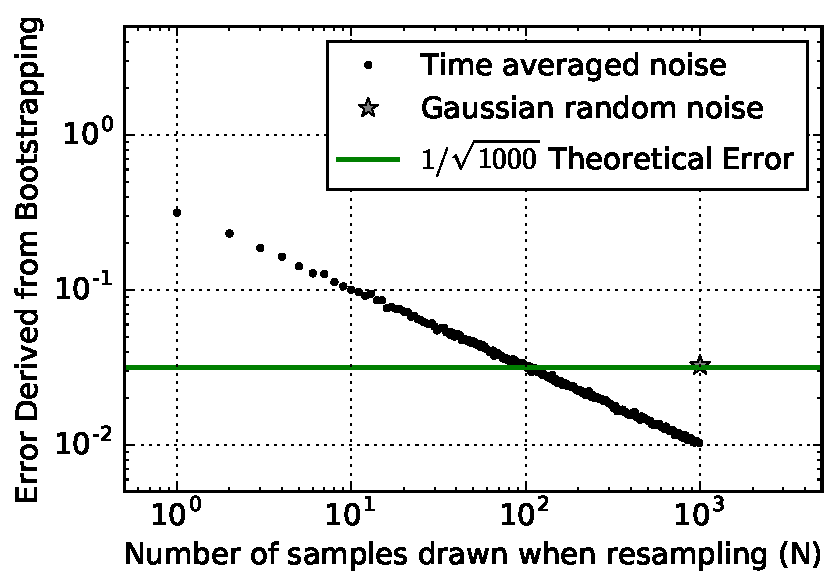
\includegraphics[trim={0cm 0cm 0cm 0cm},width=0.7\textwidth]{plots/toy_error1.pdf}
	\caption{Error estimation from bootstrapping as a function of the number of elements drawn per bootstrap when 
sampling with replacement. The star represents the standard deviation of $N_{\rm boot}=500$ bootstraps, each created by drawing $1000$ 
elements (with replacement) from a length $1000$ array of a Gaussian random signal. The black points correspond to time-averaged data (correlated data) which has $100$ independent samples. They illustrate how errors can be underestimated if 
drawing more elements than there are independent samples in the data. The estimated errors match up with the theoretical 
prediction only at $N=100$.}
	\label{fig:toy_error1}
\end{figure}

One major caveat of bootstrapping arises when working with correlated data. If, for example, a data set has many repeated 
values inside it, this would be reflected in each bootstrap. The same value would be present multiple times within a bootstrap 
and also be present between bootstraps, purely because it has a more likely chance of being drawn if there are repeats of 
itself. Therefore, bootstrapping correlated data results in a smaller variation between bootstraps, and hence, underestimates 
errors. The use of a fringe-rate filter, which averages data in time to increase sensitivity, is one example which leads to a 
reduction in the number of independent samples, creating a situation in which errors can be underestimated. We will now show 
this effect using our toy model.

Going back to our toy model, we apply a sliding boxcar average to $10$ samples at a time, thus reducing the number of 
independent data samples to $N/10 = 100$. Bootstrapping this time-averaged noise, using the same method as described 
earlier (drawing $N=1000$ elements per bootstrap sample), underestimates the error by a factor of $\sim3$ (black points in Figure \ref{fig:toy_error1}, at $N=1000$). This occurs 
because we are drawing more samples than independent ones available, and thus some samples are repeated multiple times 
in all bootstraps, leading to less variation between the bootstraps. In fact, the error derived from bootstrapping is a strong 
function of the number of elements that are drawn per bootstrap (Figure \ref{fig:toy_error1}, black points), and we can both 
underestimate the error by drawing too many or overestimate it by drawing too few. However, since we know that we have $100$ 
independent samples in this toy model, the error associated with drawing $N=100$ samples with replacement does match the theoretical prediction 
as expected (the black points cross the green line at $N=100$ in Figure \ref{fig:toy_error1}).

This example highlights the importance of understanding how analysis techniques (such as fringe-rate filtering) can affect a 
common statistical procedure like bootstrapping. Bootstrapping as a means of estimating power spectrum errors from real 
fringe-rate filtered data requires knowledge of the number of independent samples, which is not always a trivial task. For 
example, computing the effective number of independent samples of fringe-rate filtered data is not as simple as counting the 
number of averages performed. Down-sampling a time-averaged signal is straightforward using a boxcar average, but non-trivial with a more complicated convolution function that has long tails. Hence, we do not recommend bootstrapping unless the 
number of independent samples along the axis that is being re-sampled is well-determined. In Chapter \ref{sec:Boot}, we explain how we underestimated errors in the \citetalias{ali_et_al2015} analysis of PAPER and how our bootstrapping procedure has now changed to avoid the over-sampling of correlated data. 

In summary, bootstrapping can be an effective and straightforward way to estimate errors of a data set. However, we have 
illustrated a situation in which bootstrapping can lead to underestimated errors and therefore underestimated power spectrum limits. We have shown that 
bootstrapped error depends strongly on the number of elements drawn in a bootstrap sample. Estimated errors can drop to 
arbitrarily small values when the number of elements drawn exceeds the effective number of independent elements. 
%We have also shown a situation in which a bootstrapping method does not provide the most sensitive measurement possible. 
While bootstrapping is convenient because it provides a way to estimate errors from the data itself, one must assess whether certain 
analysis choices have compromised the method and whether a variation or an avoidance of traditional re-sampling could be preferred instead.

\section{Bias Toy Model}
\label{sec:BiasOverview} % make sure this is the same as original paper when put in

In a 21\,cm power spectrum, detections could be the EoR signal, but they could also 
%(and unfortunately more likely) 
be attributed to other sources of bias. Connecting a detection to EoR as opposed to noise or foreground bias is a key challenge of 
future 21\,cm data analyses \citep[e.g.][]{petrovic_and_oh2011}. In this section we will discuss possible sources of bias in a measurement, as well as techniques 
that can help mitigate their effects. We will also present a series of tests in a pedagogical fashion which we suggest be used to 
help evaluate deep limits and/or detections.

\subsection{Foreground and Noise Bias}
\label{sec:BiasTypes}

In Chapter \ref{sec:SiglossOverview}, we discussed signal loss as a form of multiplicative bias to estimates of the signal. Foregrounds are another type of bias, but an additive instead of a multiplicative one. Foreground bias is perhaps one of the main factors limiting 21\,cm results, as foreground signals lie $\sim4$-$5$ orders of 
magnitude above the cosmological signal. Though there are many techniques proposed for removing foregrounds (see e.g., \citealt{vedantham_et_al2012}; \citealt{chapman_et_al2012}; \citealt{parsons_et_al2012a}; \citealt{parsons_et_al2012b}; \citealt{dillon_et_al2013a}; \citealt{wang_et_al2013}; \citealt{parsons_et_al2014}; \citealt{liu_et_al2014a}; \citealt{wolz_et_al2014}; \citealt{liu_et_al2014b}; \citealt{dillon_et_al2015}; \citealt{pober_et_al2016a}; \citealt{trott_et_al2016}), most 
experiments currently remain limited by residuals rather than noise, especially at low $k$.

One common method to isolate and filter foregrounds is to exploit their behavior in $k$-space. For a particular 
baseline length, there is a maximum delay imposed on sources attached to the sky, which corresponds to the light-crossing time between two 
antennas in a baseline. For longer baselines, this value increases, producing what is known as "the 
wedge"
\citep{datta_et_al2010, parsons_et_al2012b, vedantham_et_al2012, pober_et_al2013, thyagarajan_et_al2013, liu_et_al2014a, liu_et_al2014b, patil_et_al2017}. 
The wedge describes a region in $k$-space contaminated by smooth spectrum foregrounds, bounded by baseline length (which is proportional to $k_{\perp}$) and delay (which is 
proportional to $k_{\parallel}$). Properties of the wedge can be used to isolate and 
%remove 
avoid foregrounds, as done by \citetalias{ali_et_al2015}, 
\citet{parsons_et_al2014}, \citet{dillon_et_al2014}, \citet{dillon_et_al2015}, \citet{jacobs_et_al2015}, \citet{beardsley_et_al2016}, and \citet{trott_et_al2016}.

Although smooth-spectrum foregrounds preferentially show up at low delay, or low $k$-modes, their isolation within the wedge is not perfect. In deep measurements, power spectrum measurements at $k_{\parallel}$ values beyond 
the delay associated with the length of a baseline are often still contaminated at a low level. This leakage, particularly at low $k$'s, can be attributed to 
convolution kernels associated with Fourier-transforming visibilities into delay-space. In other words, smooth-spectrum 
foregrounds appear as $\delta$-functions in delay-space, convolved by the Fourier transform of the source spectrum, the signal chain, and the 
antenna response, all of which could smear out the foregrounds and cause leakage outside the wedge \citep[e.g.,][]{ewall-wice_et_al2017, kerrigan_et_al2018}.

There are analysis techniques to mitigate the effects of foreground leakage and prevent information from low $k's$ from 
spreading to high $k$ values. For example, narrow window functions in delay-space can be used to minimize the leakage from a particular 
$k$ value into other ones (\citealt{liu_et_al2014b}). In other words, one can construct an estimator using QE that forces a 
window function to have a minimum response to low $k$ values. The window function used in \citetalias{ali_et_al2015} is constructed in such a way, 
specifically to prevent foregrounds that live at low $k's$ from contaminating higher $k$-modes (see Chapter \ref{sec:Bias}). 

Determining the source of positive non-EoR detections at higher $k$'s is more difficult. In previous power spectrum results, these detections have been explained as instrumental systematics, particularly time-variable cross talk, RFI, cable reflections, and calibration errors (\citetalias{ali_et_al2015}; \citealt{parsons_et_al2014}; \citealt{dillon_et_al2014}; \citealt{beardsley_et_al2016}; \citealt{patil_et_al2017}). In the next section, we will present some tests that can help distinguish these excesses from that of EoR. 

In addition to foreground bias, noise can also be responsible for positive power spectrum detections if thermal noise is 
multiplied by itself. Every 21\,cm visibility measurement contains thermal noise that is comprised of receiver and sky noise. 
We expect this noise to be independent between antennas and thus we can beat it down (increase sensitivity) by integrating 
longer, using more baselines, etc. However, the squaring of noise can occur when cross-multiplying visibilities, which is shown by 
the two copies of $\textbf{x}$ in Equation \eqref{eq:qhat}. If both copies of $\textbf{x}$ come from the same baseline and time, it 
can result in power spectrum measurements that are higher than those predicted by the thermal noise of the instrument. One 
way to avoid this type of noise bias is to avoid cross-multiplying data from the same baselines or days. This ensures that the 
two quantities that go into a measurement have separate noises that don't correlate with each other. We also note that if the noise level is known, this type of bias can be subtracted off, though this procedure is argued to be dangerous (\citealt{dillon_et_al2014}; \citealt{parsons_et_al2014}).

Another type of noise bias can stem from the spurious cross-coupling of signals between antennas. This excess is known as 
instrumental crosstalk and is an inadvertent correlation between two independent measurements via a coupled signal path. 
Crosstalk varies on a time-scale much slower than the typical fringe-rates of 
sources. Because it is slow-varying, crosstalk can be suppressed using time-averages or fringe-rate filters. However, there 
remains a possibility that power spectrum detections that aren't the cosmological signal are caused by residual, low-level crosstalk which survived any 
suppression techniques. 

\subsection{Jackknife Tests}
\label{sec:JackknifeOverview}

We now approach the difficult task of tracing excesses to foreground, noise, and EoR biases through a discussion of useful 
jackknife tests. Again, we first approach this topic pedagogically as an introduction to the related PAPER discussion in Chapter 
\ref{sec:Bias}. 

The jackknife is a resampling technique in which a statistic (i.e., power spectrum) is computed in subsets of the data (\citealt{quenouille1949}; \citealt{tukey1958}). These 
subsets are then compared to reveal systematics. In this section we define two main tests --- the null test and the traditional 
jackknife --- and explain how a power spectrum detection must pass each. We then highlight how these tests can be used to 
help distinguish between different sources of bias.
 
\begin{itemize}
\item \textbf{Null Test}: A null test is a type of jackknife test that removes the astronomical signal from data in order to 
investigate underlying systematics (see \citet{keating_et_al2016} for examples from intensity mapping that are closely related to our current application). For example, one can 
divide data into two subsets by separating odd and even Julian dates, or the first half of the observing season from the second. 
Subtracting the two removes signal that is common to both subsets, including foregrounds and the EoR signal. The resulting power 
spectrum should be consistent with thermal noise estimates; if it is not, it suggests the presence of a systematic that differs 
from one of the data subsets to the other (i.e., doesn't get subtracted perfectly). 
\item \textbf{Traditional Jackknife}: In a broader sense, it is important to perform many jackknife tests in order to instill 
confidence in a final result. A stable result must be steadfast throughout all jackknives no matter how the data is sliced. 
Jackknives can be taken along several different axes --- for example, one could start with a full data set, and compute a new 
power spectrum every time as a day of data is removed, or a baseline is removed. This type of jackknife would reveal bias 
present only at certain LSTs (such as a foreground source), for example, or misbehaving baselines.
\end{itemize}

While the null test hunts for deviations from thermal noise and the jackknife tests for deviations in subsamples, they are both 
closely related. We can highlight the connection between the two using a toy model data set.

Suppose we have four independent measurements made along two different axes. As an example, we construct $\textbf{x}_{1a}$, $\textbf{x}_{1b}$, $\textbf{x}_{2a}$, and $\textbf{x}_{2b}$, where the numbers symbolize two different days of data and the letters represent two different baselines. Each of the 
measurements have dimensions of $100$ time integrations and $20$ frequency channels. They each have separate thermal 
noises constructed as a Gaussian random signal for each, and identical EoR signals. 

To mimic the presence of a systematic, we add a toy sinusoid foreground, similar to the one used in 
Chapter \ref{sec:toymodel}, to only $\textbf{x}_{2a}$ and $\textbf{x}_{2b}$. This represents a foreground signal 
present in only the second day of data, but not the first. Mathematically, if  $\textbf{n}$ 
is noise, $\textbf{e}$ is the EoR signal, and $\textbf{f}$ is the foreground signal, the four measurements can be written as:

\begin{eqnarray}
\label{eq:bias1}
\textbf{x}_{1a} &=& \textbf{n}_{1a} + \textbf{e}  \\ 
\textbf{x}_{1b} &=& \textbf{n}_{1b} + \textbf{e}  \\ 
\textbf{x}_{2a} &=& \textbf{n}_{2a} + \textbf{e} + \textbf{f} \\ 
\textbf{x}_{2b} &=& \textbf{n}_{2b} + \textbf{e} + \textbf{f}.
\end{eqnarray} 

\noindent We now take a jackknife along the day-axis, forming separate power spectrum estimates for each day:

\begin{eqnarray}
\widehat{\textbf{P}}_{1} &\propto& \textbf{x}_{1a}\textbf{x}_{1b}^{\dagger} \\
\widehat{\textbf{P}}_{2} &\propto& \textbf{x}_{2a}\textbf{x}_{2b}^{\dagger}.
\end{eqnarray}

\begin{figure}
	\centering
	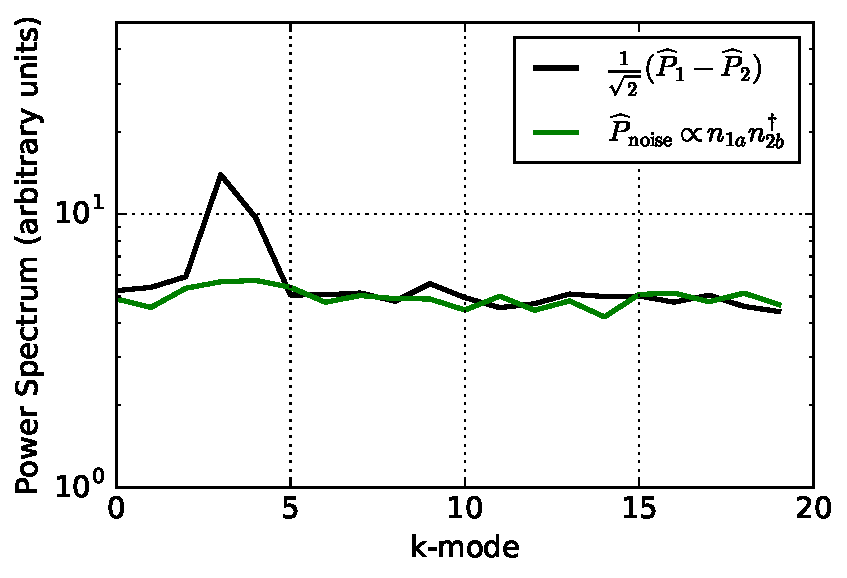
\includegraphics[trim={0cm 0cm 0cm 0cm},width=0.65\textwidth]{plots/toy_bias1.pdf}
	\caption{A null jackknife test shown as the power spectrum difference between two measurements (black), compared to the power spectrum of noise alone (green). Because the null test is not consistent with noise, it suggests the 
presence of a systematic in either $\textbf{x}_{1}$ or $\textbf{x}_{2}$. Null tests of clean measurements should be consistent 
with thermal noise.}
	\label{fig:toy_bias1}
\end{figure}

\begin{figure}
	\centering
	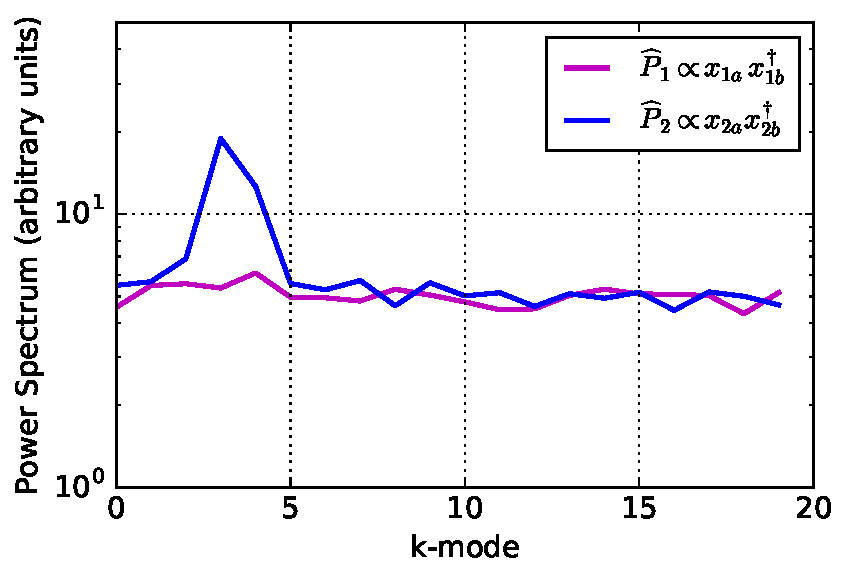
\includegraphics[trim={0cm 0cm 0cm 0cm},width=0.65\textwidth]{plots/toy_bias2.pdf}
	\caption{Power spectrum estimates for $\textbf{x}_{1}$ and $\textbf{x}_{2}$, two jackknives of the toy model. They suggest 
the presence of a systematic in $\textbf{x}_{2}$ only, illustrating how jackknives can be used to tease out excesses. Clean 
measurements should remain consistent despite the jackknife taken.}
	\label{fig:toy_bias2}
\end{figure}

We do not perform a time-average or apply a fringe-rate filter to this toy model, since we are interested only in what jackknife 
tests can tell us about biases. For the same reason, we use a weighting matrix of $\textbf{I}$ for power spectrum estimation to 
avoid signal loss. 

To construct a null test, we difference the two power spectra, with the result shown in Figure \ref{fig:toy_bias1} (black) along with the power spectrum of noise only (green). Subtracting the two estimates removes sky signal that should ideally be present in both jackknives. However, we see a clear difference between the null test and the power spectrum of 
noise. This signifies a non-EoR bias that is only present in either $\textbf{x}_{1}$ or $\textbf{x}_{2}$, but not both.

While the null test is useful for testing noise properties and the uniformity of a data set, jackknives are useful in pinpointing 
which data subsets are contaminated by biases and which are not; in our toy model we see that the bias exists only in $
\textbf{x}_{2}$ (Figure \ref{fig:toy_bias2}). If foreground or noise biases exist in a data set, jackknives can tease them out and 
provide insight into possible sources. For example, if jackknives along the time-axis reveal a bias present at a certain LST, a 
likely explanation would be excess foreground emission from a radio source in the sky at that time. A jackknife test involving 
data before and after the application of a fringe-rate filter can reveal whether crosstalk noise bias is successfully suppressed 
with the filter, or if similar-shaped detections in both power spectra suggest otherwise. There are many other jackknife axes of 
which we will not go into detail here, including baseline, frequency, and polarization. Ultimately, an EoR detection should persist 
through them all and a clean measurement should exhibit noise-like null spectra.

In this section we have highlighted how null tests and jackknife tests are key for determining the nature of a power spectrum 
detection. In Chapter \ref{sec:Bias} we perform some examples of these tests on PAPER-64 data in order to show that our 
excesses are not EoR and to identify their likely cause. 





\defcitealias{ali_et_al2015}{A15}

\chapter{PAPER-64 Case Study}
\label{c.PSA64}


\section{Overview}
\label{sec:PSA64overview}

In the previous chapter we have discussed three overarching 21\,cm power spectrum themes --- signal loss, error estimation, 
and bias. Understanding the subtleties and trade-offs involved in each is necessary for an accurate and robust understanding of 
a power spectrum result. 

We now apply these lessons to data from the PAPER experiment in order to illustrate our revised analysis pipeline. We begin with a brief overview of PAPER's data processing steps prior to power spectrum estimation before delving into each theme in detail.

\subsection{Observations}

As described in Chapter \ref{sec:PAPER_intro}, PAPER is a dedicated 21\,cm experiment located in the Karoo Desert in South Africa. The PAPER-64 configuration consists of 64 dual-polarization drift-scan elements that are arranged in a grid layout (Figure \ref{fig:ant_layout}). While every unique baseline is used for calibration, only a subset of the baselines are used for the power spectrum analysis in \citetalias{ali_et_al2015} (the three baselines used are the $30$\,m East/West baselines and their off-diagonal companions where two antennas are in adjacent columns and neighboring rows) and only one baseline-type is used for the demonstrations in this chapter (only the $30$\,m East/West baselines).

PAPER-64 conducted nighttime observations from November 2012 to March 2013. Over the course of the season, LST-coverage varied slightly, with power spectrum analyses focusing on the ``cold patch" range from $\sim0$-$8$\,hours when the Galaxy is below the horizon. The PAPER correlator processes a 100-200\,MHz bandwidth that consists of 1024 channels, each of width 97.6\,kHz. Visibilities are integrated for 10.7\,s before being written to disk. 

PAPER's raw data is compressed by a factor of $\sim70$ through the use of RFI, delay, and delay-rate filters. More specifically, radio frequency interference is flagged at the $6\sigma$ level. Next, a low-pass delay filter is applied to all the data in order to filter out delays greater than the maximum delay allowed by the longest baseline in the array. Similarly, a low-pass fringe-rate, or delay-rate filter is applied to limit fringe-rates to allowable scales set by the array. Finally, the data is decimated to critical Nyquist sampling rates of 493\,kHz and 42.9\,s. For more details about PAPER's data acquisition and compression pipelines, we refer the reader to \citet{parsons_et_al2010} and \citetalias{ali_et_al2015}.

\begin{figure}
    \centering
    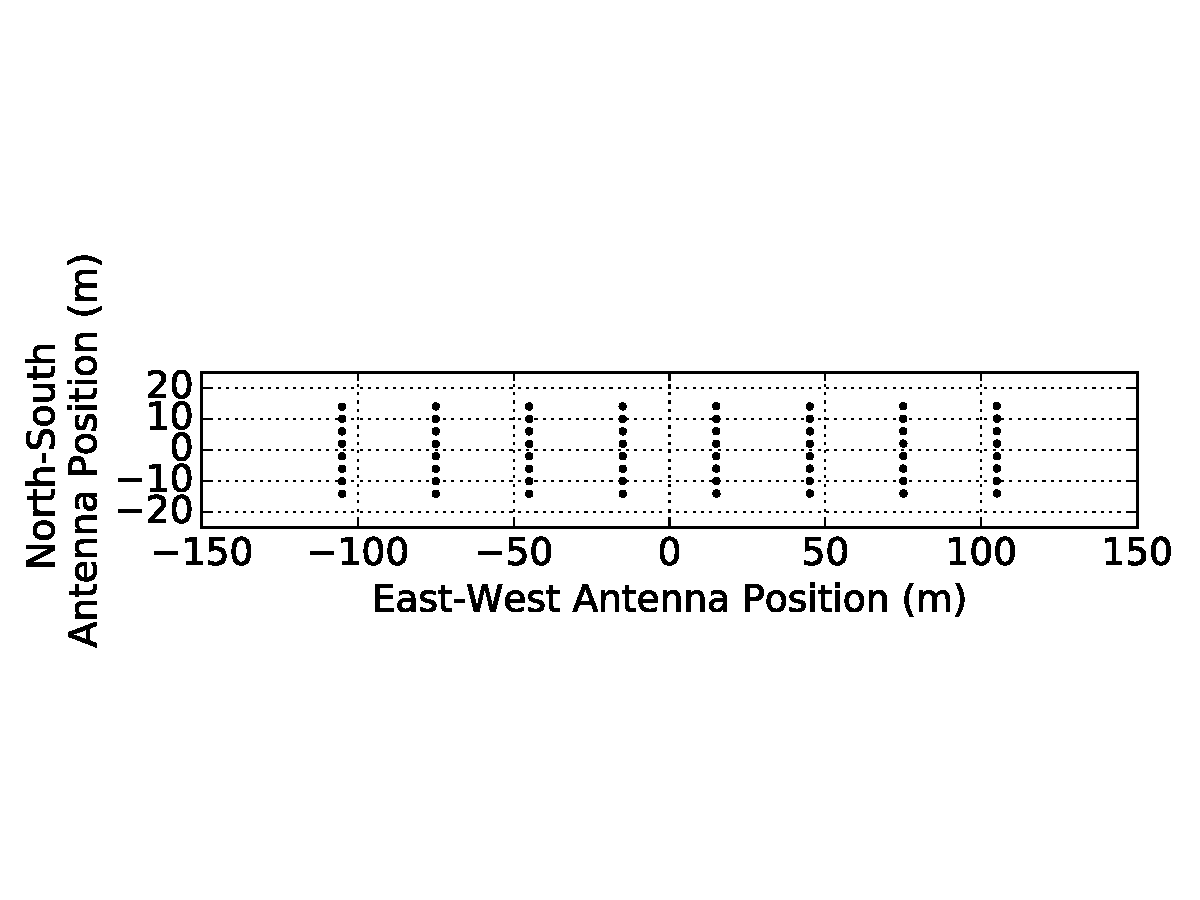
\includegraphics[trim={0cm 0cm 0cm 0cm},width=\columnwidth]{plots/ant_layout_aspect.pdf}
    \caption{The PAPER-64 antenna layout. We use only $10$ of the $30$ m East/West baselines for the analysis in this 
chapter (i.e., a subset of the shortest horizontal spacings).}
    \label{fig:ant_layout}
\end{figure}

\subsection{Data Processing}
\label{sec:PSA64_processing}

As described in Chapters \ref{sec:calibration_intro}, \ref{sec:fg_intro}, \ref{sec:frf_intro}, the primary post-processing steps of PAPER's compressed data is calibration, foreground-filtering, and fringe-rate filtering. We now give a brief overview of each, as applied to PAPER data.

We employ the package {\sc Omnical} for redundant calibration (\citealt{zheng_et_al2014}), which comprises of three steps. The first is {\tt FirstCal}, which uses all baseline redundancies to generate a static gain solution for each antenna that will unwrap any phase wrapping between two identical baselines. We perform {\tt FirstCal} because the next stage of {\sc Omnical} cannot tell the difference between a phase of $0$ and $2\pi$, for example. The second step is {\tt LogCal}, which takes the log of all the visibility equations (Equation \eqref{eq:gains}) and separates the real and imaginary components into two matrices. Coarse solutions are determined for both the antenna gains and ``model" visibilities (one for each baseline type) simultaneously. The final step of {\sc Omnical} is {\tt LinCal}, which applies small perturbations to the {\tt LogCal} solutions in an iterative fashion, honing in on the optimal solutions.
 
It is important to note that while {\sc Omnical} is powerful for ensuring array redundancy, it is not able to solve for $4$ calibration parameters - namely, the overall gain, phase, and tip/tilt of the array. For absolute calibration, we turn to a standard self-calibration routine which includes imaging Pictor A, Fornax A, and the Crab Nebula in order to fit for the overall phase solutions and the flux scale.

After calibration, we combine the XX and YY linear polarization data to form pseudo-Stokes I as defined as:

\begin{equation}
\label{eq:stokes}
V_{I} = \frac{1}{2}(V_{XX}+V_{YY})
\end{equation}
(\citealt{moore_et_al2013}).

Next, a delay-filter is used to filter out foregrounds contained inside the maximum delay set by each baseline. This is accomplished by de-convolving out our sampling function (which contains flags due to RFI) from our delay-domain visibilities using a CLEAN-like algorithm that restricts our clean components to inside the horizon limit, plus a 15\,ns buffer. The Fourier-transformed clean components are then subtracted from our visibilities. This filtering process is performed on a per-baseline, per-integration basis, and we achieve a brightness suppression of $\sim4$ orders of magnitude in our visibilities.

After delay-filtering, we perform a final round of RFI-removal by flagging visibilities that lie more than $3\sigma$ above the mean on a time, frequency, and baseline basis. Finally, we stack our data in LST into two datasets, alternating between even and odd Julian Dates to create an ``even" and ``odd" LST-binned dataset. A total of 124 days of data are included in the LST-binned dataset.

The final step before power spectrum estimation is fringe-rate filtering. The chosen filter (which is described in the next section) is applied on a per-baseline basis and weights the fringe-rate bins on the sky by the RMS of the primary beam at that same location. A smooth filter is constructed by fitting a Gaussian to the filter shape in the fringe-rate domain. Additionally, fringe-rates below 0.2\,mHz are zeroed out, effectively removing slowly-varying signals such as crosstalk. We then convolve our time-domain visibilities by the Fourier-transform of the fringe-rate filter to yield time-averaged visibilities that have gained another order of magnitude in sensitivity.

\subsection{Case Study Data}

For the case study presented in the rest of this chapter, we 
focus on a subset of the PAPER-64 data used in \citetalias{ali_et_al2015}, namely, on LST-binned, Stokes I estimated data \citep{moore_et_al2013} from PAPER's $30$ m East/West baselines (Figure 
\ref{fig:ant_layout}). Hence, all data processing steps are identical to those in \citetalias{ali_et_al2015} until after the LST-binning step in Figure 3 of \citetalias{ali_et_al2015}.

The previously best published 21\,cm upper limit result from \citetalias{ali_et_al2015} placed a $2\sigma$ upper limit 
on $\Delta^{2}(k)$, defined as

\begin{equation}
\Delta^{\textbf{2}}(k) = \frac{k^{3}}{2\pi^{2}}\,\hat{P}(k),
\end{equation}

\noindent of $(22.4$ mK$)^{2}$ in the range $0.15 < k < 0.5$\,$h$ Mpc$^{-1}$ at $z = 8.4$. The need to revise this limit stems mostly from previously under-estimated signal loss and under-estimated error bars, both of which we 
address in the following sections. 

For the analysis in this chapter, we use $8.1$ hours of LST, namely an RA range of $0.5$-$8.6$ hours (\citetalias{ali_et_al2015} uses a slightly longer RA 
range of $0$-$8.6$ hours; we found that some early LSTs were more severely foreground contaminated). We also use only $10$ baselines, a subset of the $51$ total East/West baselines used in \citetalias{ali_et_al2015}, in order to illustrate our revised methods. All power spectrum results are produced for a center frequency of 151\,MHz using a width of 10\,MHz ($20$ channels), identical to the analysis in \citetalias{ali_et_al2015}. In the case study in this chapter, we only use one baseline type instead of the three as in 
\citetalias{ali_et_al2015}, but Kolopanis et al. (\textit{in prep.}) uses the full dataset presented in \citetalias{ali_et_al2015} to revise the result and place limits on the EoR at multiple redshifts (using a straightforward and not lossy approach to avoid many of the issues presented in this chapter).

The most significant changes from \citetalias{ali_et_al2015} occur in our revised power spectrum analysis, which is explained in the rest of this chapter, but we also note that the applied fringe-rate filter is also slightly different. In \citetalias{ali_et_al2015}, the 
applied filter was not equivalent to the optimal fringe-rate filter (which is designed to maximize power spectrum sensitivity). Instead, the optimal filter was degraded slightly by widening it in fringe-rate space. This was chosen in order to increase the number of independent 
modes and reduce signal loss associated with the quadratic estimator, though as we will explain in the next section, this signal loss was still under-estimated. With the development of a new, 
robust method for assessing signal loss, we choose to use the optimal filter in order to maximize sensitivity. This filter is 
computed for a fiducial 30\,m baseline at 150\,MHz, the center frequency in our band. The filter in both the fringe-rate 
domain and time domain is shown in Figure \ref{fig:frp}.

Finally, we emphasize that the discussion that follows is solely focused on signal loss associated with empirical covariance weighting. As mentioned in Chapter \ref{sec:SiglossOverview}, there are a number of steps in our analysis pipeline which could lead to loss, including gain calibration, delay filtering, and fringe-rate filtering, which have been investigated at various levels of detail in \citet{parsons_et_al2014} and \citetalias{ali_et_al2015} but are clearly the subject of future work. Here we only focus on the most significant source of loss we have identified and note that Kolopanis et al. (\textit{in prep.}) and other future work will consider additional sources of signal loss and exercise increased caution in reporting results.

\begin{figure}
    \centering
    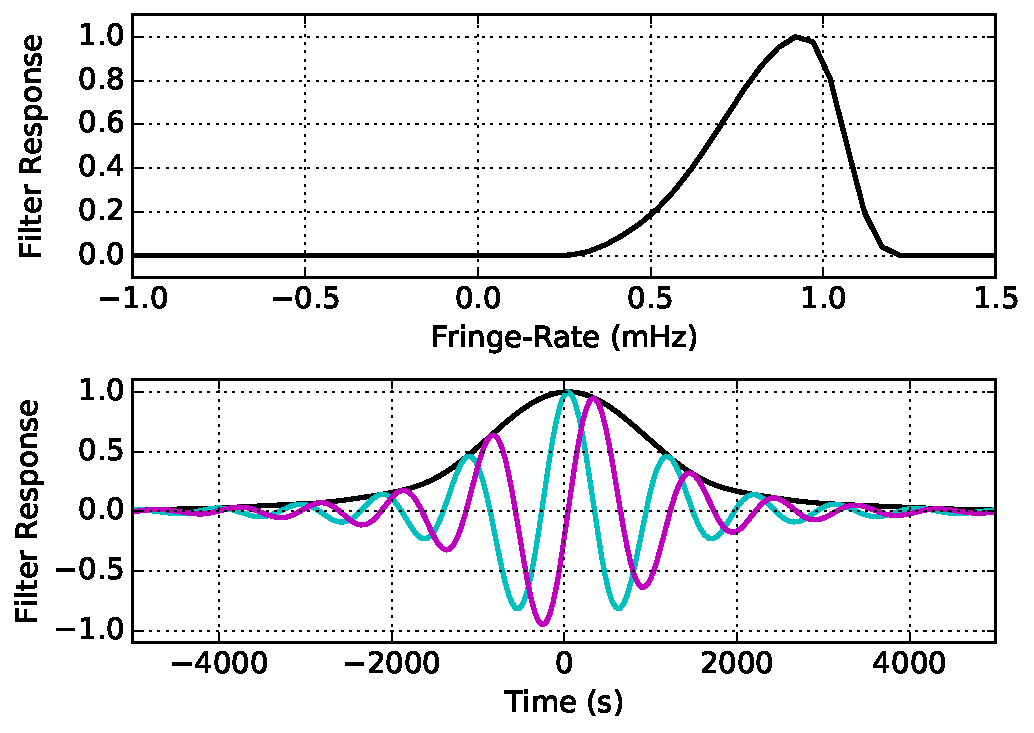
\includegraphics[width=0.6\textwidth]{plots/frp.pdf}
    \caption{Top: the normalized optimal power-spectrum sensitivity weighting in fringe-rate space for our fiducial baseline and 
Stokes I polarization beam. Bottom: the time domain convolution kernel corresponding to the top panel. Real and imaginary 
components are illustrated in cyan and magenta, respectively, with the absolute amplitude in black. The fringe-rate filter acts as 
an integration in time, increasing sensitivity but reducing the number of independent samples in the dataset.}
    \label{fig:frp}
\end{figure}

\section{Signal Loss}
\label{sec:CaseStudy}

We present our PAPER-64 signal loss investigation in three parts. We first give an overview of our signal injection framework which is used to estimate loss (Chapter \ref{sec:siglossmethod}). In this framework (and as in \citetalias{ali_et_al2015}), we inject simulated cosmological signals into our data and test the recovery of those signals (an approach also taken by \citet{masui_et_al2013}). As we will see, correlations between the injected signals and the data are significant complicating factors which were previously not taken into account. Next, we describe our methodology in practice and detail how we map our simulations into a posterior for the EoR signal (Chapter \ref{sec:Practice}). Finally, we build off of the previous section by experimenting with different regularization schemes on PAPER data in order to minimize loss (Chapter \ref{sec:Weight}). Throughout each section, we also highlight major differences from the signal loss computation used in \citetalias{ali_et_al2015}.

\subsection{Signal Loss Methodology} 
\label{sec:siglossmethod}
In short, our method for estimating signal loss consists of adding an EoR-like signal into visibility data and then measuring how much of this injected signal would be detectable given any attenuation of this signal by the (lossy) data analysis pipeline.  To capture the full statistical likelihood of signal loss, one requires a quick way to generate many realizations of simulated 21\,cm signal visibilities. Here we use the same method as in \citetalias{ali_et_al2015}, where mock Gaussian noise visibilities (mock EoR signals) 
are filtered in time using an optimal fringe-rate filter to retain only ``sky-like" modes. Since the optimal filter has a shape that matches the rate of the sidereal motion of the sky, this transforms the Gaussian noise into a measurement that PAPER could make. This signal is then added to the visibility data.\footnote{One 
specific change from \citetalias{ali_et_al2015} is that we add this simulated signal - which has been fringe-rate filtered once already in order to transform it into a ``sky-like" signal - into the analysis pipeline before a fringe-rate filter is 
applied to the data (i.e., prior to the analysis step of fringe-rate filtering). Previously, the addition was done after the fringe-rate filter analysis step.  This change results in an increased 
estimate of signal loss, %(by a factor of $\sim$$10$), 
likely due to the use of the fringe-rate filter as a simulator. However, this pipeline difference, while significant, is not the dominant reason why signal loss was underestimated in \citetalias{ali_et_al2015} (the dominant reason is explained in the main text in Chapter \ref{sec:siglossmethod}).}

Mathematically, suppose that $\textbf{e}$ is the mock injected EoR signal (at some amplitude level). We do not know the true EoR signal contained within our visibility data, $\textbf{x}$, so $\textbf{e}$ takes on the role of the true EoR signal (for which we measure its loss). Furthermore, one can make the assumption that the true EoR signal is small within our measured data, so the data vector $\textbf{x}$ itself is representative of mostly contaminants. Using this assumption, the sum of $\textbf{x}$ and $\textbf{e}$, defined as $\textbf{r}$:

\begin{equation}
\label{eq:rxe}
\textbf{r} = \textbf{x} + \textbf{e},
\end{equation}
can be thought of as the sum of contaminants plus EoR. The quantity $\textbf{r}$ then becomes the dataset for which we are measuring how much loss of $\textbf{e}$ there is due to our power spectrum pipeline.

We are interested in quantifying how much variance in $\textbf{e}$ is lost after weighting $\textbf{r}$ and estimating the power 
spectrum according to QE formalism. We investigate this by comparing two quantities we call the input power spectrum and 
output power spectrum: $\widehat{P}_{\rm in}$ and $\widehat{P}_{\rm out}$, estimated using QE as

\begin{equation}
\label{eq:Pin}
\widehat{P}_{\rm in}^{\alpha} \equiv \text{M}^{\alpha}_{\rm in}\textbf{e}^{\dagger}\textbf{I}\textbf{Q}^{\alpha}\textbf{I}\textbf{e}
\end{equation}

\noindent and

\begin{eqnarray}
\label{eq:sigloss}
\widehat{P}_{\rm out}^{\alpha} &\equiv& \widehat{\textbf{P}}_{r}^{\alpha} \nonumber\\%-\widehat{\textbf{P}}_{x,\alpha} \nonumber \\
&=& \text{M}^{\alpha}_{r}\textbf{r}^{\dagger}\textbf{R}_{r}\textbf{Q}^{\alpha}\textbf{R}_{r}\textbf{r},% - \text{M}^{\alpha}_{x}\textbf{x}^{\dagger}\textbf{R}_{x}\textbf{Q}^{\alpha}\textbf{R}_{x}\textbf{x},
\end{eqnarray}
where, for illustrative purposes and notational simplicity, we have written these equations with scalar normalizations M, even though for our numerical results we choose a diagonal matrix normalization using $\mathbf{M}$ as in Equation \eqref{eq:phat}.

The quantity $\widehat{P}_{\rm in}$, defined by Equation \eqref{eq:Pin}, is a uniformly weighted estimator of the power spectrum of $\mathbf{e}$. It can be considered the power spectrum of this particular realization of the EoR; alternatively, it can be viewed as the true power spectrum of the injected signal up to cosmic variance fluctuations. The role of $\widehat{P}_{\rm in}$ in our analysis is to serve as a reference for the power spectrum that would be measured if there were no signal loss or other systematics. The input power spectrum is then to be compared to $\widehat{P}_{\rm out}$, which approximates the (lossy) power spectrum estimate that is output by our analysis pipeline prior to any signal loss adjustments. 

Under this injection framework, we can begin to see explicitly why there can be large signal loss. Expanding out Equation \eqref{eq:sigloss}, $\widehat{P}_{\rm out}$ becomes:

\begin{eqnarray}
\label{eq:crossterm_full}
\widehat{P}_{\rm out}^{\alpha} &=& \text{M}^{\alpha}_{r}(\textbf{x}+\textbf{e})^{\dagger}\textbf{R}_{r}\textbf{Q}^{\alpha}\textbf{R}_{r}(\textbf{x}+\textbf{e}) \nonumber \\%- 
%\text{M}^{\alpha}_{x}\textbf{x}^{\dagger}\textbf{R}_{x}\textbf{Q}^{\alpha}\textbf{R}_{x}\textbf{x} \nonumber \\
&=& \text{M}^{\alpha}_{a}\textbf{x}^{\dagger}\textbf{R}_{r}\textbf{Q}^{\alpha}\textbf{R}_{r}\textbf{x} + \text{M}^{\alpha}_{b}\textbf{e}^{\dagger}\textbf{R}_{r}\textbf{Q}
^{\alpha}\textbf{R}_{r}\textbf{e} \nonumber \\
&+& \text{M}^{\alpha}_{c}\textbf{x}^{\dagger}\textbf{R}_{r}\textbf{Q}^{\alpha}\textbf{R}_{r}\textbf{e} + \text{M}^{\alpha}_{d}\textbf{e}^{\dagger}\textbf{R}_{r}\textbf{Q}^{\alpha}\textbf{R}_{r}\textbf{x}. %\nonumber \\
%&-& \text{M}^{\alpha}_{x}\textbf{x}^{\dagger}\textbf{R}_{x}\textbf{Q}^{\alpha}\textbf{R}_{x}\textbf{x}.
\end{eqnarray}
Assuming \textbf{R}$_{r}$ is symmetric, the two cross-terms (terms with one copy of $\textbf{e}$ and one copy of $\textbf{x}$) can be summed together as:

\begin{eqnarray}
\label{eq:crossterm}
\widehat{P}_{\rm out}^{\alpha} &= &  \text{M}^{\alpha}_{a}\textbf{x}^{\dagger}\textbf{R}_{r}\textbf{Q}^{\alpha}\textbf{R}_{r}\textbf{x} + \text{M}^{\alpha}_{b}\textbf{e}^{\dagger}\textbf{R}_{r}\textbf{Q}
^{\alpha}\textbf{R}_{r}\textbf{e} \nonumber \\
&+& 2 \text{M}^{\alpha}_{c}\textbf{x}^{\dagger}\textbf{R}_{r}\textbf{Q}^{\alpha}\textbf{R}_{r}\textbf{e}. %\nonumber \\
%&-& \text{M}^{\alpha}_{x}\textbf{x}^{\dagger}\textbf{R}_{x}\textbf{Q}^{\alpha}\textbf{R}_{x}\textbf{x}.
\end{eqnarray}
One of the key takeaways of this section is that the \citetalias{ali_et_al2015} analysis estimated signal loss by comparing \textit{only} the signal-only term (second term in Equation \eqref{eq:crossterm}) with $\widehat{P}_{\rm in}$, whereas in fact the cross-term (third term in Equation \eqref{eq:crossterm}) can substantially lower $\widehat{P}_{\rm out}$. In order to investigate the effect of each of these terms on signal loss, all three components are plotted in Figure \ref{fig:sigloss_terms} for two cases: empirically estimated inverse covariance weighting ($\textbf{R}_{r} \equiv \widehat{\textbf{C}}_{r}^{-1}$) and uniform weighting ($\textbf{R}_{r} \equiv \textbf{I}$). We will now go into further detail and examine the behavior of this equation in three different regimes of the injected signal - very weak (left ends of the $P_{\rm in}$ axes in Figure \ref{fig:sigloss_terms}), very strong (right ends), and in between (middle portions).

{\bf Small injection:}
In this regime, the cross-terms (red) behave as noise averaged over a finite number of samples. Output values are Gaussian distributed around zero, spanning a range of values set by the injection level. This is because $\widehat{\textbf{R}}_{r}$ is dominated by the data $\textbf{x}$, avoiding correlations with $\textbf{e}$ that can lead to solely negative power (explained further below). In fact, for the uniformly weighted case, the cross-term  $\text{M}^{\alpha}_{x}\textbf{x}^{\dagger}\textbf{I}\textbf{Q}^{\alpha}\textbf{I}\textbf{e}$ is well modeled as a symmetric distribution with zero mean and width $\sqrt{\widehat{\textbf{P}}_e}\sqrt{\widehat{\textbf{P}}_x}$. We also note that in this regime, $\widehat{\textbf{P}}_{r}$ (black) approaches the data-only power spectrum value (gray) as expected. 

{\bf Large injection:}
When the injected signal is much larger than the measured power spectrum, the data-only components can 
be neglected as they are many orders of magnitude smaller. We include a description of this regime for completeness in our discussion, but note that the upper limits that we compute are typically not determined by simulations in this regime (i.e., in using an empirical weighting scheme we've assumed the data to be dominated by foregrounds rather than the cosmological signal).  However, it is useful as a check of our system in a relatively simple case. As we can see from Figure \ref{fig:sigloss_terms}, the cross-terms (red) are small in comparison to the signal-only term (green). Here only does the signal-only term used in \citetalias{ali_et_al2015} dominate the total power output. We again see that, in the empirical inverse covariance weighted case, the cross-terms behave as noise (positive and negative fluctuations around zero mean). This is for the same reason as at small injections --- here $\widehat{\textbf{C}}_{r}$ is dominated by the signal $\textbf{e}$. The cross-correlation can again be modeled as a symmetric distribution of zero mean and width $\sqrt{\widehat{\textbf{P}}_e}\sqrt{\widehat{\textbf{P}}_x}$.

{\bf In between:}
When the injected signal is of a similar amplitude to the data by itself, the situation becomes less straightforward. We see that 
the weighted injected power spectrum component mirrors the input power indicating little loss (i.e., the green curve follows the dotted black line), eventually 
departing from unity when the injected amplitude is well above the level of the data power spectrum. However, 
in this regime the cross-term (red) has nearly the same amplitude, but with a negative sign. As explained below, this negativity is the result of cross-correlating inverse covariance weighted terms.  This negative component drives down the $\widehat{P}_{\rm out}$ estimator (black). Again, we emphasize that in \citetalias{ali_et_al2015}, signal loss was computed by only looking at the second term in Equation \eqref{eq:crossterm} (green), which incorrectly implies no loss at the data-only power spectrum level. Ignoring the effect of the negative power from the cross-terms is the main reason for underestimating power spectrum limits in \citetalias{ali_et_al2015}.

\begin{figure*}
	\centering
	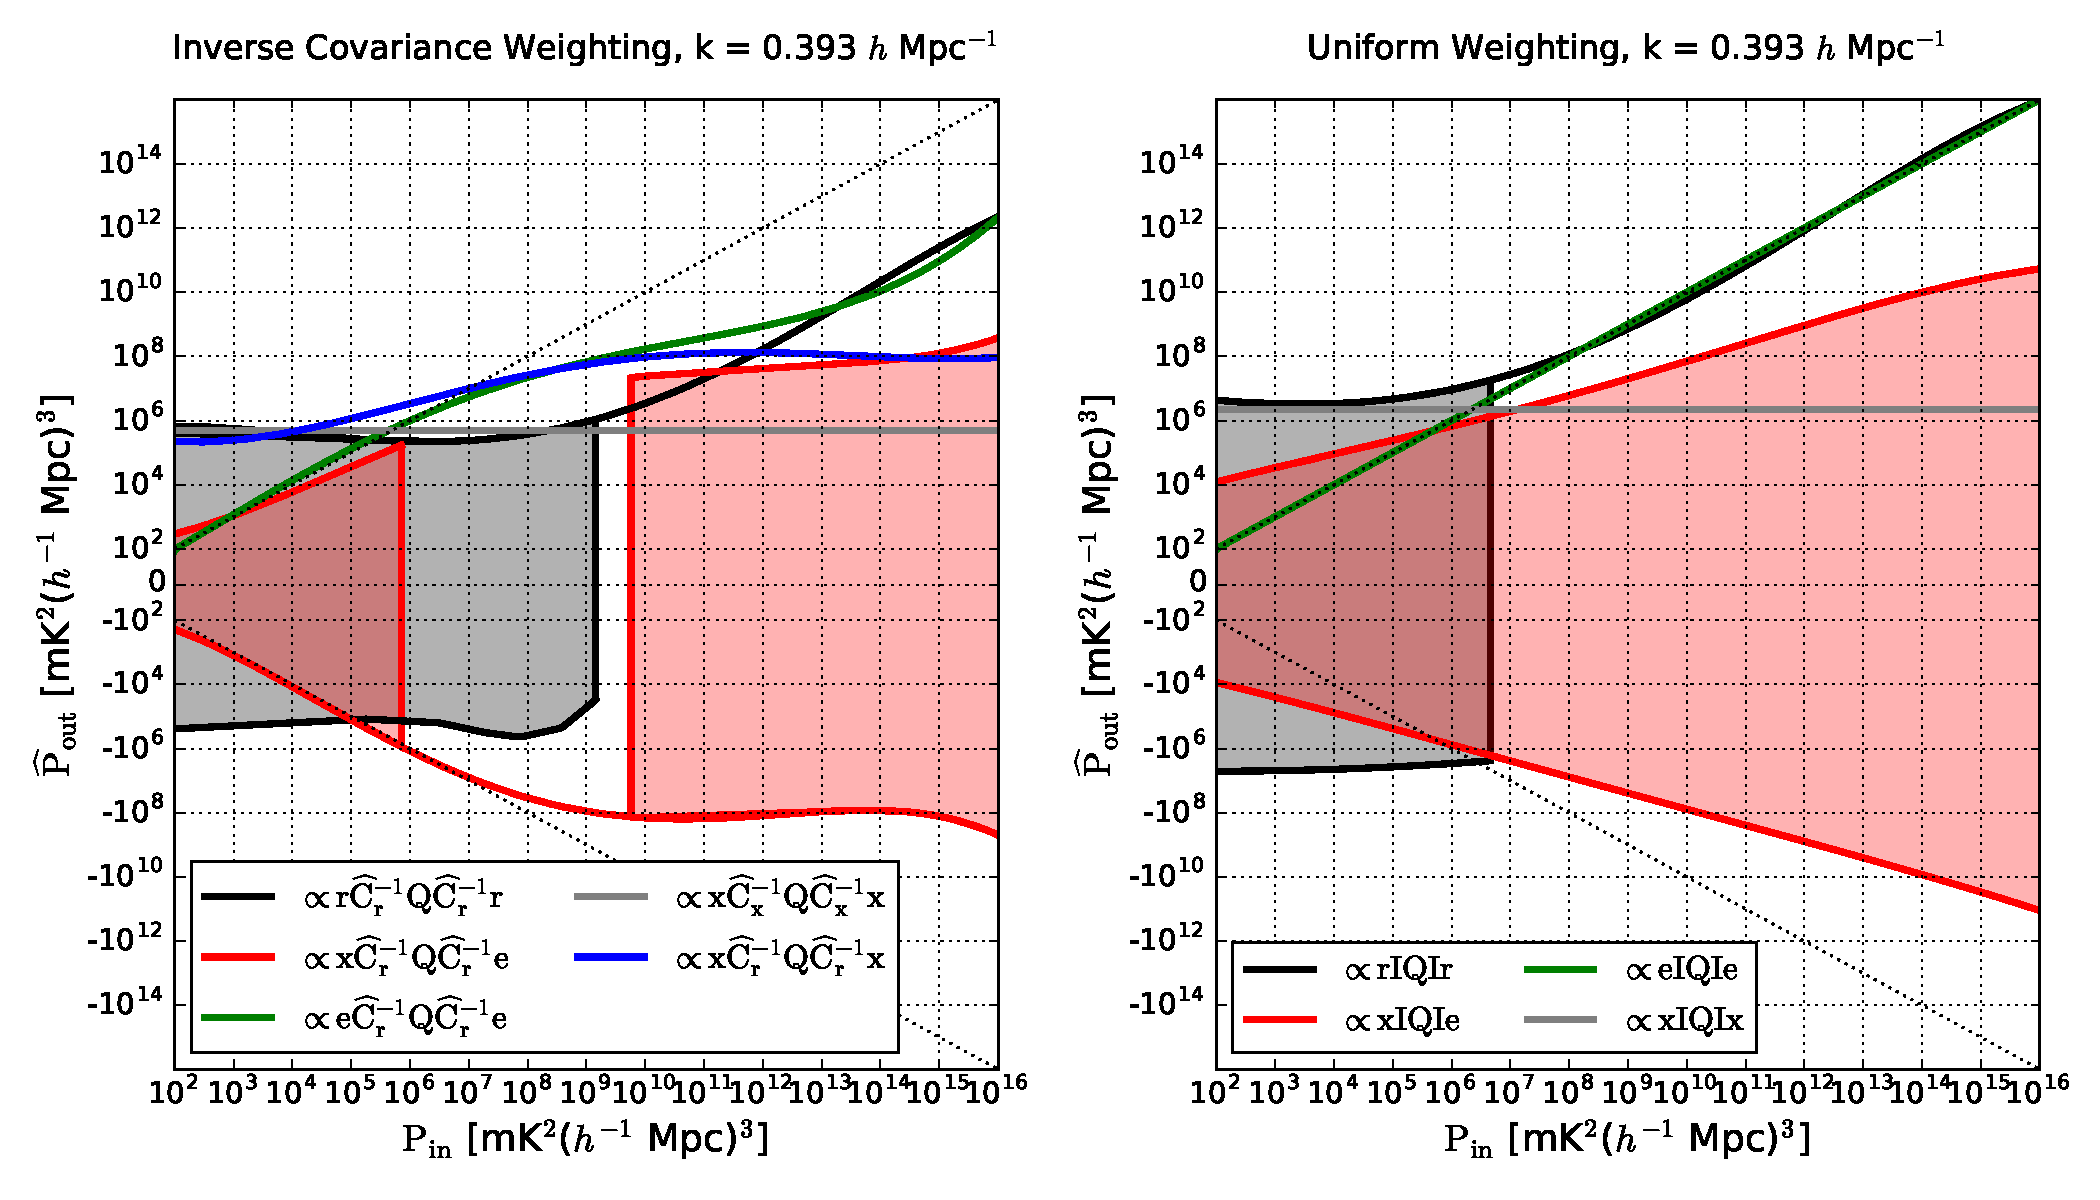
\includegraphics[width=1\textwidth]{plots/sigloss_terms.pdf}
	\caption{Illustration of the power spectrum amplitude of five different power spectrum terms, each a function of visibility data ($\textbf{x}$), simulated injected EoR signal ($\textbf{e}$), or both ($\textbf{r}$). This figure shows how these quantities behave as the power level of the injected EoR signal increases (along the x-axis).  The details of the simulation used to generate the figure is explained in Chapter \ref{sec:Practice}; here we sample a larger $P_{\rm in}$ range and fit smooth polynomials to our data points to make an illustrative example. We emphasize that the output power spectrum in black ($\widehat{P}_{\rm out}=\widehat{\textbf{P}}_r$) approximates the (lossy) power spectrum estimate that is output by our analysis pipeline prior to any signal loss adjustments. Roughly speaking, it can be compared to the input signal level ($P_{\rm in}$) to estimate the amount of signal loss. Left: Empirical inverse covariance weighting is used in power spectrum estimation, as done in \citet{ali_et_al2015}. The dotted diagonal black line indicates perfect 1:1 input-to-output mapping (no signal loss). The gray horizontal line is the power spectrum value of data alone, $\widehat{\textbf{P}}_{x}$ (it does not depend on injected power). The green signal-signal component is the term used in \citet{ali_et_al2015} to estimate signal loss. It is significantly higher than $\widehat{\textbf{P}}_{r}$ (black) when the cross-terms (red) are large and negative (black $=$ green $+$ red $+$ blue). In the regime where cross-correlations between signal and data are not dominant (small and large $P_{\rm in}$), the cross-terms have a noise-like term with width $\sqrt{\widehat{\textbf{P}}_e}\sqrt{\widehat{\textbf{P}}_x}$. However, at power levels comparable to the data (the middle region), the cross-terms can produce large, negative estimates due to couplings between $\textbf{x}$ and $\textbf{e}$ which affect $\widehat{\textbf{C}}_{r}$. This causes the difference between the green curve (which exhibits negligible loss at the data-only power spectrum value) and the black curve (which exhibits $\sim4$ orders of magnitude of loss). Right: The same power spectrum terms illustrated for the uniform weighted case.}
\label{fig:sigloss_terms}
\end{figure*}

The source of the strong negative cross-term is not immediately obvious, however it is an explainable effect. 
When $\textbf{R}_{r}$
is taken to be $\widehat{\textbf{C}}_{r}^{-1}$, the third term of Equation \eqref{eq:crossterm} is a cross-correlation between $\widehat{\textbf{C}}_{r}^{-1}\textbf{x}$ and
$\widehat{\textbf{C}}_{r}^{-1}\textbf{e}$. As shown in \citet{switzer_et_al2015}, this cross-correlation term is non-zero, and in fact negative in expectation. 
This negative cross-term power arises from a coupling between the inverse of 
$\widehat{\textbf{C}}_{r}$ and $\mathbf{x}$. 
Intuitively, we can see this by expanding the empirical covariance of $\textbf{r}=\textbf{x}+\textbf{e}$:

\begin{eqnarray}
\widehat{\textbf{C}}_{r} &=& \langle \textbf{rr}^{\dagger} \rangle_{t} \nonumber \\ 
&=& \langle \textbf{xx}^{\dagger} \rangle_{t} + \langle \textbf{xe}^{\dagger} \rangle_{t} + \langle \textbf{ex}^{\dagger} \rangle_{t} + \langle 
\textbf{ee}^{\dagger} \rangle_{t},
\end{eqnarray}

\noindent where we can neglect the first term because $\textbf{x}$ is small (i.e., the large negative cross-term power in the left panel of Figure \ref{fig:sigloss_terms} occurs when the injected amplitude surpasses the level of the data-only power spectrum).  Without loss of generality, we will assume
an eigenbasis of $\textbf{e}$, so that $\langle 
\textbf{ee}^{\dagger} \rangle_{t}$ is diagonal. The middle 
two terms, however, can have power in their off-diagonal terms due to the fact that, when averaging over a finite
ensemble, $\langle\textbf{xe}^\dagger\rangle_t$ is not zero.  As shown in Appendix C of \citet{parsons_et_al2014}%\footnote{This same appendix also gives a now-prescient warning about signal loss and the dangers of noise and sample variance in inverse covariance.}
, to leading order the inversion of a diagonal-dominant matrix like $\widehat{\textbf{C}}_{r}$ (from $\langle 
\textbf{ee}^{\dagger} \rangle_{t}$) with smaller
off-diagonal terms results in a new diagonal-dominant matrix with negative off-diagonal terms. These off-diagonal
terms depend on both $\textbf{x}$ and $\textbf{e}$. Then, when $\widehat{\textbf{C}}^{-1}_{r}$ is multiplied into $\textbf{x}$,
the result is a vector that is similar to $\textbf{x}$ but
contains a residual correlation to $\textbf{e}$ from the off-diagonal components of $\widehat{\textbf{C}}^{-1}_{r}$. The
correlation is negative because the product $\widehat{\textbf{C}}_r^{-1}\textbf{x}$ effectively squares the $\textbf{x}$-dependence
of the off-diagonal terms in $\widehat{\textbf{C}}^{-1}_{r}$ while retaining the negative sign that arose from the inversion
of a diagonal-dominant matrix.

{\bf In general:} Another way to phrase the shortcoming of the empirical inverse covariance estimator is that it is not properly normalized. Signal loss due to couplings between the data and its weightings arise because our unnormalized quadratic estimator from Equation \eqref{eq:qhat} ceases to be a quadratic quantity, and instead contains higher order powers of the data. However, the normalization matrix $\mathbf{M}$ is derived assuming that the unnormalized estimator is quadratic in the data. The power spectrum estimate will therefore be incorrectly normalized, which manifests as signal loss. We leave a full analytic solution for $\mathbf{M}$ for future work, since our simulations already capture the full phenomenology of signal loss and have the added benefit of being more easily generalizable in the face of non-Gaussian systematics.

\subsection{Signal Loss in Practice}
\label{sec:Practice}

We now shift our attention towards computing upper limits on the EoR signal for the fringe-rate filtered PAPER-64 dataset in a way that accounts for signal loss. While our methodology 
outlined below is independent of weighting scheme, here we demonstrate the computation using empirically estimated inverse covariance weighting 
($\textbf{R} \equiv \widehat{\textbf{C}}^{-1}$), the weighting scheme used in \citetalias{ali_et_al2015} which leads to substantial loss. 

One issue to address is how one incorporates the randomness of $\widehat{P}_{\rm out}$ into our signal loss corrections. A different realization of the mock EoR signal is injected with each bootstrap run, causing the output to vary in three ways ---  there is noise variation from the bootstraps, there is cosmic variation from generating multiple realizations of the mock EoR signal, and there is a variation caused by whether the injected signal looks more or less ``like'' the data (i.e., how much coupling there is, which affects how much loss results). 

For each injection level, the true $P_{\rm in}$ is simply the average of our bootstrapped estimates $\widehat{P}_{\rm in}$, since $\widehat{P}_{\rm in, \alpha}$ is by construction an unbiased estimator. Phrased in the context of Bayes' rule, we wish to find the posterior probability distribution $p(P_{\rm in} | 
\widehat{P}_{\rm out})$, which is the probability of $P_{\rm in}$ given the uncorrected/measured power spectrum estimate $\widehat{P}_{\rm out}$.  Bayes' rule relates the posterior, which we don't know, to the likelihood, which we can forward model. In other words,

\begin{equation}
\label{eq:Bayes}
p(P_{\rm in} | \widehat{P}_{\rm out}) \propto {\mathcal{L} (  \widehat{P}_{\rm out} | P_{\rm in})}\,p(P_{\rm in}) ,
\end{equation}

\noindent where $\mathcal{L} $ is the likelihood function defined 
as the distribution of data plus signal injection ($\widehat{P}_{\rm out}$) given the injection $P_{\rm in}$.  We construct this distribution  
by fixing $P_{\rm in}$ and simulating our analysis pipeline for many realizations of the injected EoR signal 
consistent with this power spectrum. The resulting distribution is normalized such that the sum over $\widehat{P}_{\rm out}$ is unity, and the 
whole process is then repeated for a different value of $P_{\rm in}$. 

The implementation details of the injection process require some more detailed explanation. In our code, we add a new realization of EoR to each independent bootstrap of data (see Chapter \ref{sec:Boot} for a description of PAPER's bootstrapping routine) with the goal of simultaneously capturing cosmic variance, noise variance, and signal loss. To limit computing time we perform $20$ realizations of each $P_{\rm in}$ level. We also run $50$ total EoR injection levels, yielding $P_{\rm in}$ values that range from $\sim$$10^{5}$\,mK$^{2}$ ($h^{-1}$ Mpc)$^{3}$ to $\sim$10$^{11}$\,mK$^{2}$ ($h^{-1}$ Mpc)$^{3}$, resulting in a total of $1000$ data points on our $P_{\rm in}$ vs. $\widehat{P}_{\rm out}$ grid. 

Going forward, we treat every $k$-value separately in order to determine an upper limit on the EoR signal per $k$. We bin our simulation outputs along the $P_{\rm in}$ axis (one bin per injection level) and, since they are well-approximated by a Gaussian distribution in our numerical results, we smooth the distribution of $\widehat{P}_{\rm out}$ values by fitting Gaussians for each bin based on its mean and variance (and normalize them). Stitching all of them together results in a 2-dimensional transfer function --- the likelihood function in Bayes' rule, namely $\mathcal{L} (  \widehat{P}_{\rm out} | P_{\rm in})$. We then have a choice for our prior, $p(P_{\rm in})$, and we choose to invoke a Jeffreys prior (\citealt{jaynes1968}) because it is a true uninformative prior for a parameter space using Bayesian probability. %For a derivation and more details about the Jeffreys prior used in our analysis, see Appendix \ref{sec:jeffreys}.

The Jeffreys prior is defined as:

\begin{equation}
\label{eq:jeffreys}
p(P_{\rm in}) \propto \sqrt {\Bigg\langle \Bigg(\frac{\partial \mathcal{L}}{\partial P_{\rm in}} \Bigg)^{2}\Bigg\rangle},
\end{equation}

\noindent where

\begin{equation}
\label{eq:logprob}
\mathcal{L} = \mathrm{ln} \, p(\widehat{P}_{\rm out} | P_{\rm in}),
\end{equation}

\noindent recalling that in our framework $P_{\rm in}$ is the power spectrum of the EoR signal (uniformly weighted), and $\widehat{P}_{\rm out}$ is the weighted output power spectrum of the data plus EoR.

Since, for a single injection amplitude, our bootstrapped $\widehat{P}_{\rm out}$ values are well-approximated by a Gaussian distribution, we can write: 

\begin{equation}
\label{eq:prob}
p(y | x) = \frac{1}{\sigma(x) \sqrt{2\pi}} e^{-\frac{1}{2}\big(\frac{y-\bar y(x)}{\sigma}\big)^{2}},
\end{equation}

\noindent simplifying our notation so that $x = P_{\rm in}$, $y = \widehat{P}_{\rm out}$, $\sigma$ is the standard deviation of $\widehat{P}_{\rm out}$, and $\bar y$ is the mean of $\widehat{P}_{\rm out}$. Using Equations \eqref{eq:prob} and \eqref{eq:logprob}, the quantity inside the expectation value of Equation \eqref{eq:jeffreys} becomes:

\begin{eqnarray}
\Big(\frac{\partial \mathcal{L}}{\partial x} \Big)^{2} &=& \frac{1}{\sigma^{2}}\Big(\frac{\partial \sigma}{\partial x}\Big)^{2} -  \Big(\frac{2(y-\bar y)}{\sigma^{3}}\Big)\frac{\partial \sigma}{\partial x}\frac{\partial \bar y}{\partial x} - \Big(\frac{2(y-\bar y)^{2}}{\sigma^{4}}\Big)\Big(\frac{\partial \sigma}{\partial x}\Big)^{2} \nonumber \\
&+& \Big(\frac{(y-\bar y)^{2}}{\sigma^{4}}\Big)\Big(\frac{\partial \bar y}{\partial x}\Big)^{2} + \Big(\frac{2(y-\bar y)^{3}}{\sigma^{5}}\Big)\frac{\partial \sigma}{\partial x}\frac{\partial \bar y}{\partial x} + \Big(\frac{(y-\bar y)^{4}}{\sigma^{6}}\Big)\Big(\frac{\partial \sigma}{\partial x}\Big)^{2}.
\end{eqnarray}

Taking the expectation value then removes all terms with odd powers of $(y - \bar y)$ because those Gaussian moments evaluate to zero. Additionally, the second moment can be simplified since $\langle (y - \bar y)^{2} \rangle = \sigma^{2}$ and the fourth moment can be simplified since $\langle (y - \bar y)^{4} \rangle = 3\sigma^{4}$. Finally, after some additional simplification the Jeffreys prior becomes:

\begin{equation}
\label{eq:jeffreys_final}
p(x) \propto \sqrt{ \frac{1}{\sigma^{2}}\Big(2\Big(\frac{\partial \sigma}{\partial x}\Big)^{2} + \Big(\frac{\partial \bar y}{\partial x}\Big)^{2}\Big) }.
\end{equation}

When we simulate our full injection framework, we note that the prior is set to zero outside our injection range. For the injections that we do sample, we can simply fit analytic functions to the mean and standard deviations of $\widehat{P}_{\rm out}$ ($\bar y$ and $\sigma$) as functions of $P_{\rm in}$. An example of the typical shape of these functions for the PAPER-64 analysis is shown in Figure \ref{fig:jeffreys1}, though in practice we fit solutions for every $k$-value and simulation independently.

\begin{figure}
	\centering
	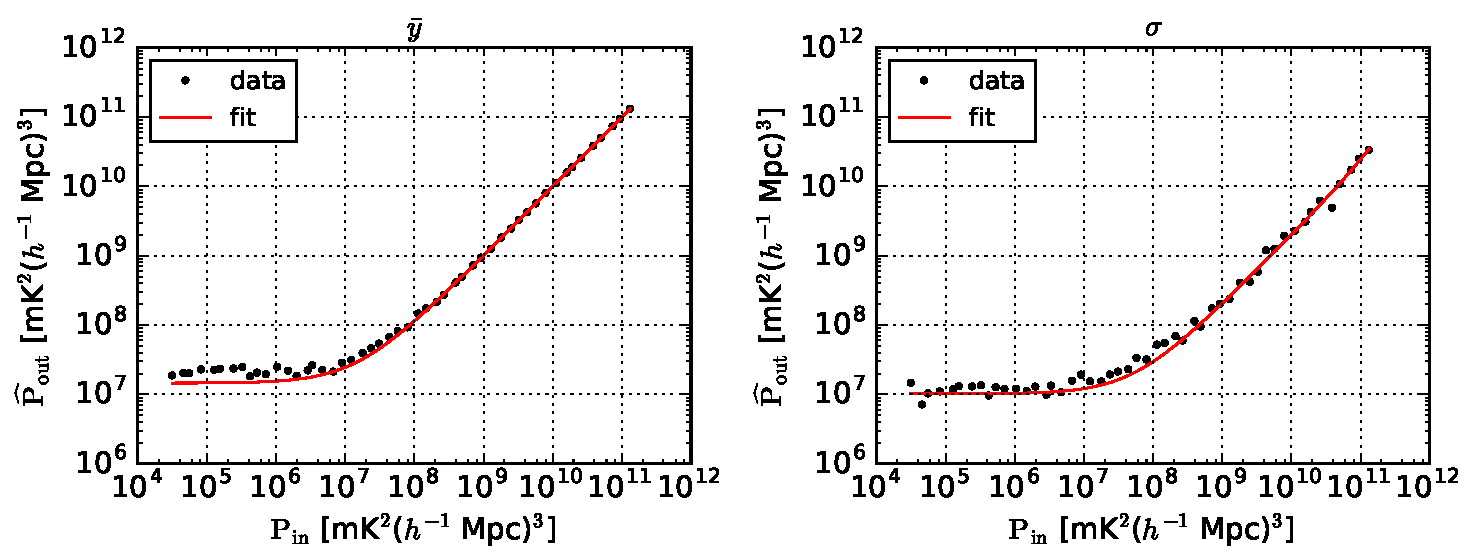
\includegraphics[width=\columnwidth]{plots/jeffrey_fits.pdf}
	\caption{An illustrative example (for the PAPER-64 analysis using uniform weighting and $k=0.393$\,$h$ Mpc$^{-1}$) of how the mean of $P_{\rm out}$ (left) and standard deviation of $P_{\rm out}$ (right) behave as a function of $P_{\rm in}$. Polynomials are fit to each (red) to describe how $\bar y$ and $\sigma$ evolve with $x$ (injection level), respectively, for the computation of the Jeffreys prior as defined in Equation \eqref{eq:jeffreys_final}. The polynomial fits for this example are $y = (-5.1 \times 10^{-15})x^{2} + x + (1.5 \times 10^{7})$ and $y = (5.0 \times 10^{-13})x^{2} + 0.2 x + 10^{7}$ for $\bar y$ and $\sigma$, respectively.}
	\label{fig:jeffreys1}
\end{figure}

We also show the typical shape of the Jeffreys prior used in our analysis in Figure \ref{fig:jeffreys2}, as computed by Equation \eqref{eq:jeffreys_final}. Most noticeably, it is not constant with $P_{\rm in}$, meaning a uniform prior, which is often used for simplicity, is informative in our application. Therefore, due to its objective nature we choose to use a Jeffreys prior in our analysis, multiplying our likelihood functions by Equation \eqref{eq:jeffreys_final} before computing posterior distributions.

\begin{figure}
	\centering
	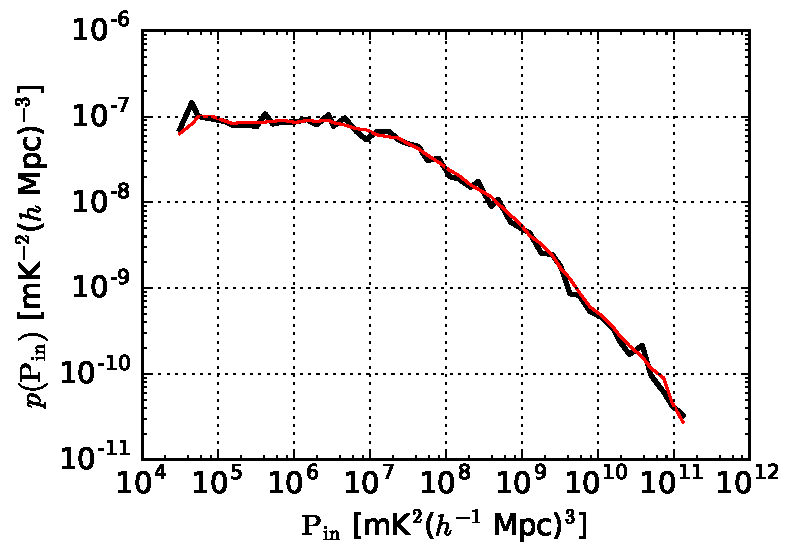
\includegraphics[width=10cm]{plots/jeffrey_prior.pdf}
	\caption{An example of the typical Jeffreys prior shape for the PAPER-64 analysis as computed by Equation \eqref{eq:jeffreys_final} (black). We smooth the prior using a sliding boxcar average over every $5$ injection levels (red). Most noticeably, the Jeffreys prior is not constant with $P_{\rm in}$, meaning a uniform prior would be an informative prior.}
	\label{fig:jeffreys2}
\end{figure}

Finally, our transfer functions are shown in Figure \ref{fig:sigloss_transfercurve} for both the weighted (left) and unweighted (right) cases. Our bootstrapped power spectrum outputs are shown as black points and the colored heat-map overlaid on top is the likelihood function modified by our prior. Although we only show figures for one $k$-value, we note that 
the shape of the transfer curve is similar for all $k$'s. We then invoke Bayes' interpretation and re-interpret it as the posterior $p(P_{\rm in}|\widehat{P}_{\rm out})$ where we recall that $\widehat{P}_{\rm out}$ represents a (lossy) power spectrum. To do this we make a horizontal cut across at the data value $\widehat{\textbf{P}}_{x}$ (setting $\widehat{P}_{\rm out} = \widehat{\textbf{P}}_{x}$), shown by the gray solid line, to yield a posterior distribution for the signal. We normalize this final distribution and compute the $95\%$ confidence interval (an upper limit on EoR).

By-eye inspection of the transfer function in Figure \ref{fig:sigloss_transfercurve} gives a sense of what the signal loss result should be. The power spectrum value of our data, $
\widehat{\textbf{P}}_{x}$ is marked by the solid gray horizontal lines. From the left plot (empirically estimated inverse covariance weighting), one can eyeball that a data value of $10^{5} \,$mK$^{2}$ ($h^{-1}$ Mpc)$^{3}$, for example, would map approximately to an upper limit of $\sim10^{9} \,$mK$^{2}$ ($h^{-1}$ Mpc)$^{3}$, implying a signal loss factor of $\sim10^{4}$. 

\begin{figure*}
	\centering
	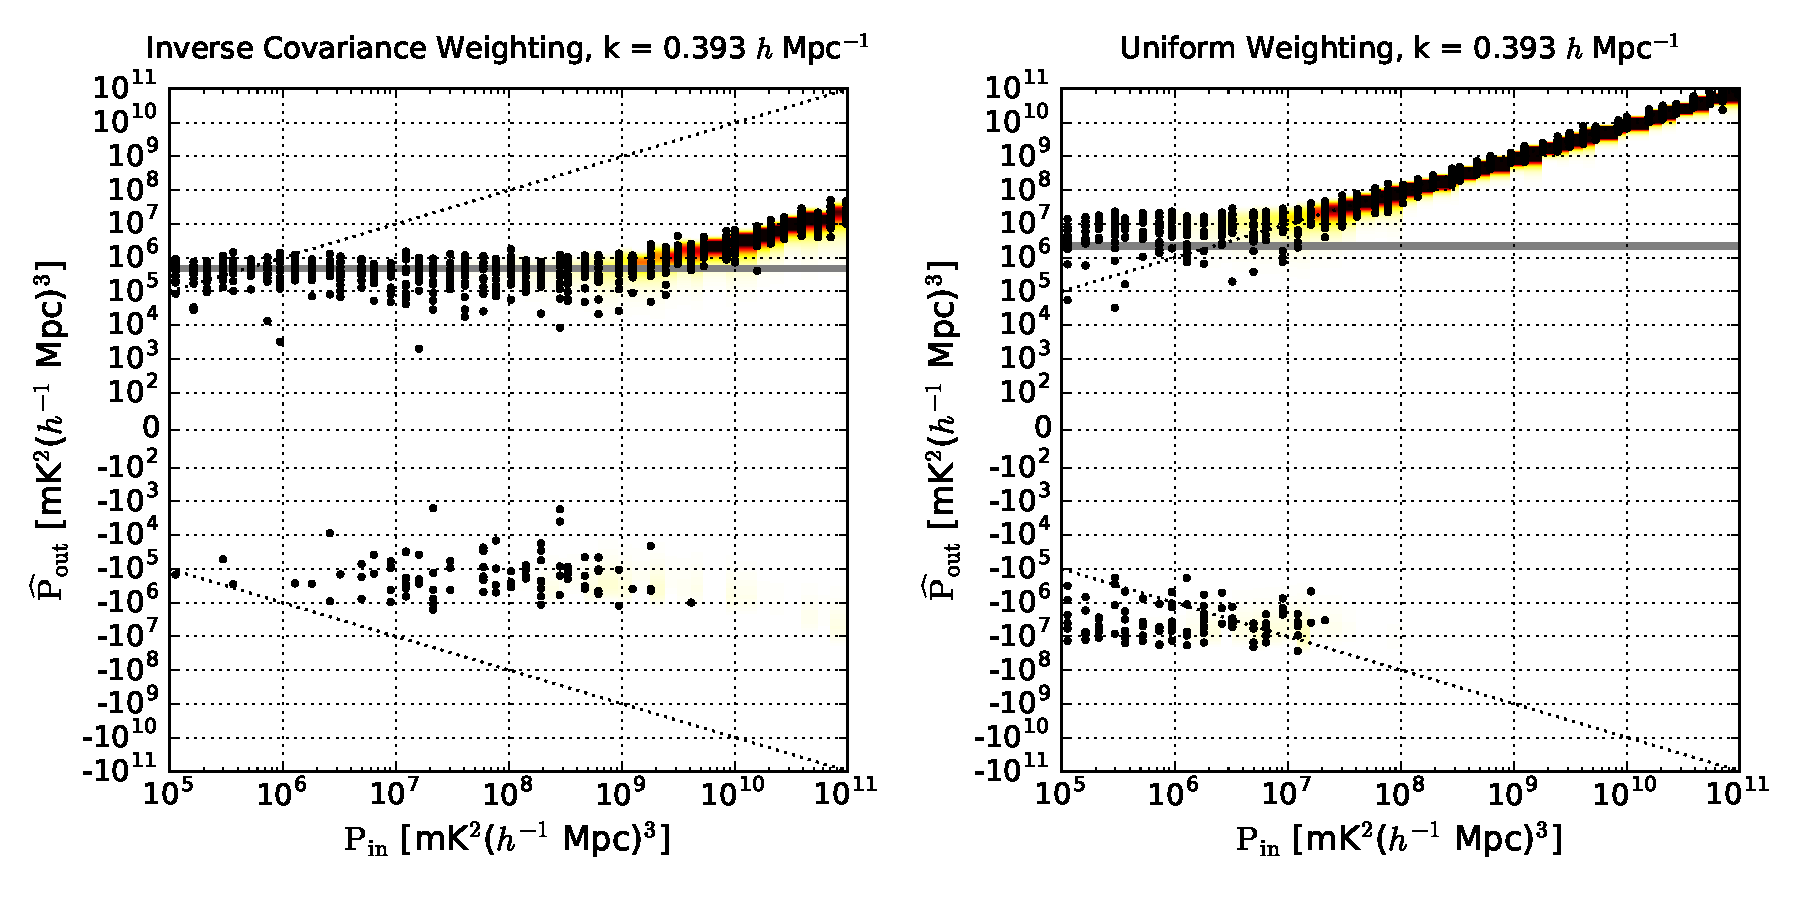
\includegraphics[width=1\textwidth]{plots/sigloss_transfercurve_posneg.pdf}
	\caption{Signal loss transfer functions showing the relationship of $P_{\rm in}$ and $\widehat{P}_{\rm out}$, as defined by Equations \eqref{eq:Pin} and \eqref{eq:sigloss}. Power spectra values (black points) are generated for $20$ realizations of $\textbf{e}$ per signal injection level. Since our $\widehat{P}_{\rm out}$ values are well-approximated by a Gaussian distribution, we fit Gaussians to each injection level based on the mean and variance of the simulation outputs. This entire likelihood function is then multiplied by a Jeffreys prior for $p(P_{\rm in}$), with the final result shown as the colored 
heat-maps on top of the points. Two cases are displayed: empirically estimated inverse covariance weighted PAPER-64 data (left) and uniform-weighted data (right). The dotted black 
diagonal lines mark a perfect unity mapping, and the solid gray horizontal line denotes the power spectrum value of the data $\widehat{\textbf{P}}_{x}$, from which a posterior distribution for the signal is extracted. From these plots, it is clear that the weighted case results in $\sim4$ orders of magnitude of signal loss at the data-only power spectrum value, whereas the uniform-weighted case does 
not exhibit loss. The general shape of these transfer functions are also shown by the black curves in Figure \ref{fig:sigloss_terms} for comparison.}
	\label{fig:sigloss_transfercurve}
\end{figure*}

The loss-corrected power spectrum limit for empirically estimated inverse covariance weighted PAPER-64 data is shown in Figure \ref{fig:ps2_data} (solid red), which we can compare to the original lossy result (dashed red). Post-signal loss estimation, the power spectrum limits are higher than both the theoretical noise level (green) and uniform-weighted power spectrum (which is shown three ways: black and gray points are positive and negative power spectrum values, respectively, with $2\sigma$ error bars from bootstrapping, the solid blue is the upper limit on the EoR signal using the full signal injection framework, and the shaded gray is the power spectrum values with thermal noise errors). We elaborate on this point in the next section, as well as investigate alternate 
weighting schemes to inverse covariance weighting, with the goal of finding one that balances the aggressiveness of down-weighting contaminants and minimizing the loss of the EoR signal. 

\begin{figure*}
	\centering
	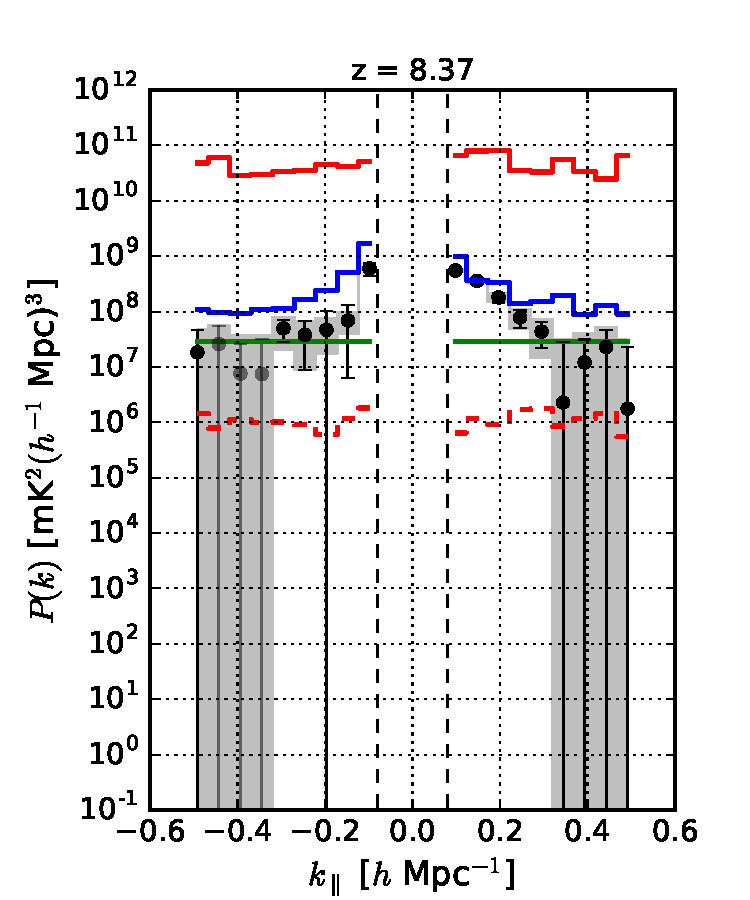
\includegraphics[width=0.45\textwidth]{plots/ps1_data.pdf}
	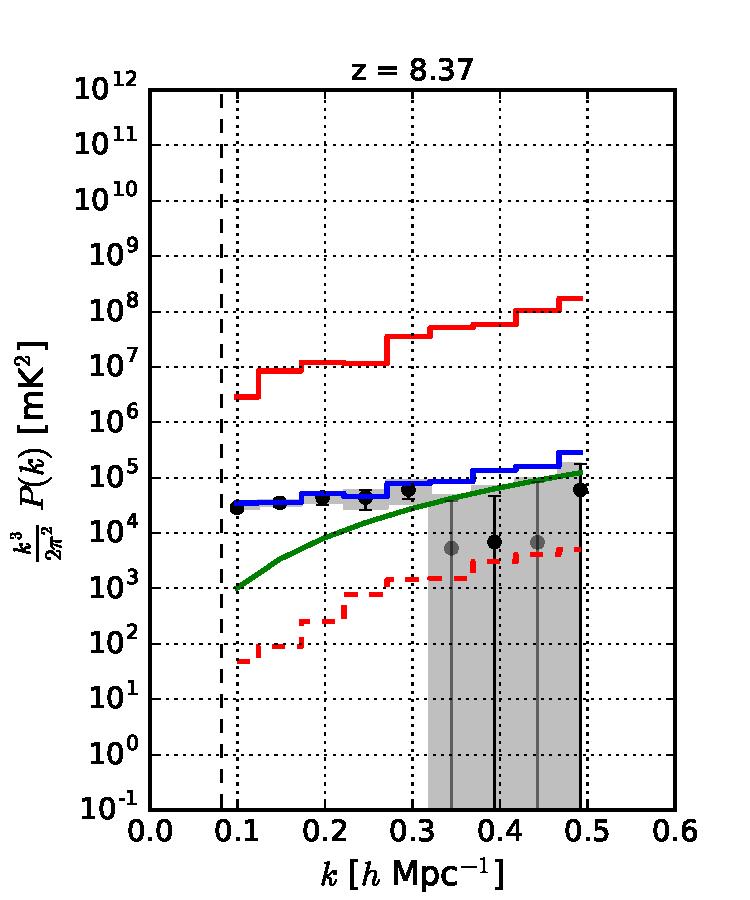
\includegraphics[width=0.45\textwidth]{plots/ps2_data.pdf}
	\caption{A power spectrum of a subset of PAPER-64 data illustrating the use of empirical inverse covariance weighting. The solid red curve is the $2\sigma$ upper limit on the EoR signal estimated from our signal injection framework using empirical inverse covariance weighting. Shown for comparison is the lossy limit prior to signal loss estimation (dashed red). The theoretical $2\sigma$ thermal noise level prediction based on observational parameters is in green, whose calculation is detailed in Chapter \ref{sec:Error}. Additionally, the power spectrum result for the uniform weighted case is shown in three different ways: power spectrum values (black and gray points as positive and negative values, respectively, with $2\sigma$ error bars from bootstrapping), the $2\sigma$ upper limit on the EoR signal using our full signal injection framework (solid blue), and the measured power spectrum values with $2\sigma$ thermal noise errors (gray shaded regions). The vertical dashed black lines signify the horizon limit for this analysis using $30$\,m baselines. In this example, we see that the lossy power spectrum limit is $\sim 4$ orders of magnitude too low when using empirical inverse covariance weighting.}
\label{fig:ps2_data}
\end{figure*}

\subsection{Minimizing Signal Loss}
\label{sec:Weight}

With a signal loss formalism established, we now have the capability of experimenting 
with different weighting options for $\textbf{R}$. Our goal here is to choose a weighting method that successfully down-weights 
foregrounds and systematics in our data without generating large amounts of signal loss as we have seen with the inverse covariance estimator. We have found that the balance 
between the two is a delicate one and requires a careful understanding and altering of empirical covariances. 

We saw in Chapter \ref{sec:otherweight} how limiting the number of down-weighted eigenmodes (i.e., flattening out part of the 
eigenspectrum and effectively decoupling the lowest-valued eigenmodes, which are typically EoR-dominated, from the data) can help minimize signal loss. We experiment with this idea on PAPER-64 data, dialing the number of modes 
that are down-weighted from zero (which is equivalent to identity-weighting, or the uniform-weighted case) to $21$ (which is the full inverse 
covariance estimator). The power spectrum results for one $k$-value, both before and after signal loss 
estimation, are shown in the top panel in Figure \ref{fig:sigloss_modeloop}. We see that the amount of signal loss increases as weighting 
becomes more aggressive (dashed red). In other words, more EoR-dominated fluctuations are being overfit and 
subtracted as more modes are down-weighted. We also find that the power spectrum upper limit, post-signal loss estimation, 
increases with the number of down-weighted modes (solid red). The more modes we use in down-weighting, the stronger the coupling between the weighting and the data, and the greater the error we have in estimating the power spectrum. \citet{switzer_et_al2013} took a similar approach in determining the optimal number of modes to down-weight in GBT data, finding similar trends and noting that removing too few modes is limited by residual foregrounds and removing too many modes is limited by large error bars and signal loss.

Optimistically, we expect there to be a ``sweet spot" as we dial our regularization knob; a level of regularization where weighting 
is beneficial compared to uniform weighting (blue). In other words, we would like a weighting scheme that down-weights eigenmodes that predominantly describe foreground modes, but not EoR modes. We see in Figure \ref{fig:sigloss_modeloop} that this occurs roughly when 
only the $\sim3$ highest-valued eigenmodes are down-weighted and the rest are given equal weights (though for the case shown, weighting only slightly outperforms uniform weighting). For a similar discussion on projecting out modes (zeroing out eigenmodes, rather than just ignoring their relative weightings as we do in this study), see \citet{switzer_et_al2013}. 

We also saw in Chapter \ref{sec:otherweight} how adding the identity matrix to the empirical covariance can minimize signal loss. We experiment with this idea as well, shown in the bottom panel of Figure \ref{fig:sigloss_modeloop}. The dashed red and solid red lines represent power spectrum limits pre and post-signal loss estimation, respectively, as a function of the strength of $\textbf{I}$ that is added to $\widehat{\textbf{C}}$, quantified as a percentage of Tr($\widehat{\textbf{C}})\textbf{I}$ added to $\widehat{\textbf{C}}$. We parameterize this ``regularization strength" parameter as $\gamma$, namely $\widehat{\textbf{C}} \equiv \widehat{\textbf{C}} + \gamma$Tr$(\widehat{\textbf{C}})\textbf{I}$. From this plot we see that only a small percentage of Tr($\widehat{\textbf{C}})$ is needed to significantly reduce loss. We expect that as the strength of $\textbf{I}$ is increased (going to the left), both the red curves will approach the uniform-weighted case. We also notice that the post-signal loss limit hovers around the uniform-weighted limit for a large range of regularization strengths and while an overall trend from high-to-low signal loss is seen as the strength increases, there does not appear to be a clear ``minimum" that produces the least loss.

\begin{figure*}
	\centering
	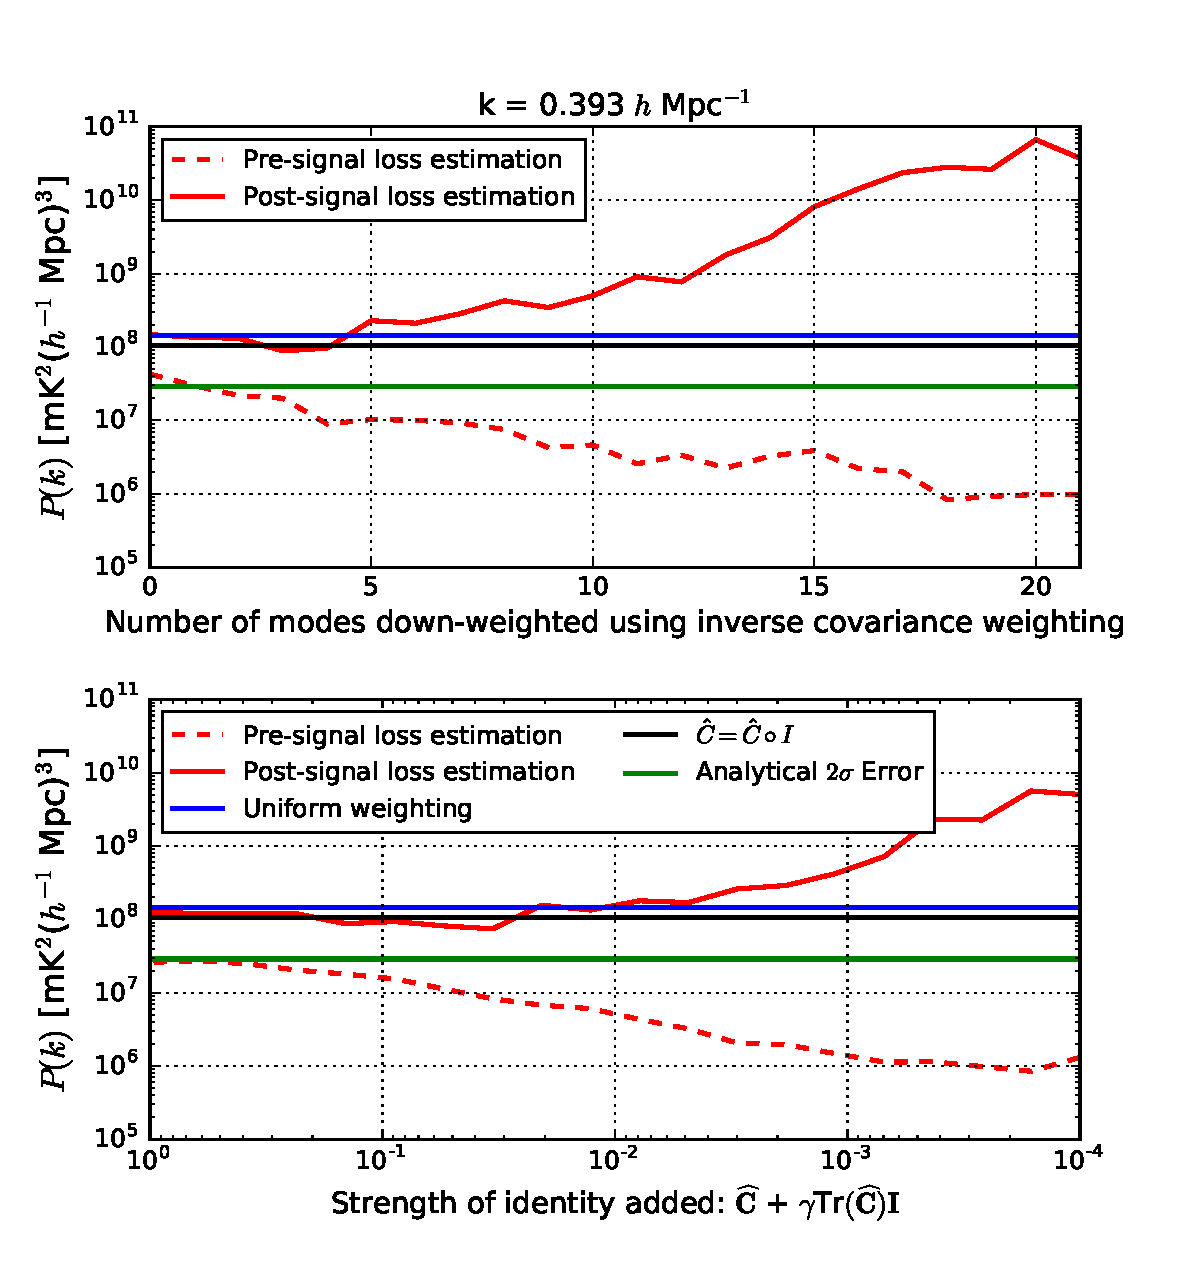
\includegraphics[width=.7\textwidth]{plots/sigloss_modeloop_2panel.pdf}
	\caption{Power spectra $2\sigma$ upper limits for $k=0.393$\,$h$ Mpc$^{-1}$ for fringe-rate filtered PAPER-64 data. Top: Values 
are shown before (dashed red) and after (solid red) signal loss estimation via our signal injection framework as a function of number of eigenmodes of $\widehat{\textbf{C}}$ that 
are down-weighted. This regularization knob is tuned from $0$ modes on the left (i.e., unweighted) to $21$ modes on the right (i.e., the full inverse 
covariance estimator). $\sim4$ orders of magnitude of signal loss results when using empirically estimated inverse covariance weighting. Bottom: Power spectrum upper limits before (dashed red) and after (solid red) signal loss estimation as a function of identity added to the empirical covariance. This regularization knob is tuned from $\gamma = 10^{-4}$ on the right (i.e., very little regularization) to $\gamma = 1$ on the left (see main text for the definition of $\gamma$). Also 
plotted in both panels for comparison are $2\sigma$ power spectrum upper limits for the uniform-weighted case (blue) and inverse variance 
weighted case (black); both are after signal loss estimation. Finally, a theoretical prediction for noise ($2\sigma$ error) is plotted 
as green. In the PAPER-64 analysis in this paper, we choose to use a regularization scheme of $\widehat{\textbf{C}}_{\rm eff} \equiv 0.09 \, $Tr($\widehat{\textbf{C}})\textbf{I} + \widehat{\textbf{C}}$ ($\gamma = 0.09$) as a simple example of regularization that minimizes loss, and note that the power spectrum limits using this type of regularization are roughly constant across a large range of values of $\gamma$.}
	\label{fig:sigloss_modeloop}
\end{figure*}

In addition to our thermal noise prediction (green) and uniform-weighted power spectrum limit (blue), one additional horizontal line is shown in Figure \ref{fig:sigloss_modeloop} 
in both panels and represents a third regularization technique. This line (black) denotes the power spectrum value, post-signal loss estimation, for inverse variance weighting (multiplying an identity 
matrix element-wise to $\widehat{\textbf{C}}$). This result is single-valued and not a function of the horizontal axis. We see that all three regularization schemes shown (solid red top panel, solid red bottom panel, black) perform similarly at 
their best (i.e., when $\sim3$ eigenmodes are down-weighted in the case of the top panel's solid red curve). However, for the remainder of this paper, we choose to use the weighting option of $\widehat{\textbf{C}} + 0.09 \,$Tr($\widehat{\textbf{C}})\textbf{I}$, or $\gamma = 0.09$, which we will denote as $\widehat{\textbf{C}}_{\rm eff}$. We choose this weighting scheme merely as a simple example of regularizing PAPER-64 covariances, noting that the power spectrum upper limit remains roughly constant for a broad range of values of $\gamma$. 

It is important to note that our signal injection methodology for assessing loss makes the assumption that we know the true signal's strength and structure. Realistically, these details about the EoR signal are unknown and our signal loss framework is limited by our simulations. Therefore, while this paper employs this methodology as an example of one way of estimating loss, Kolopanis et al. (\textit{in prep.}) use uniform weightings in order to produce more trustworthy, straightforward power spectrum limits that do not suffer from loss.

The power spectrum result for our subset of PAPER-64 data (using only one baseline separation type, $10$ baselines, and $\widehat{\textbf{C}}_{\rm eff}$) using the analysis presented in this paper is shown in Figure 
\ref{fig:ps1_data}. Again, the solid red curve represents our upper limit on the EoR signal using the full signal injection framework. The uniform weighted case is shown as the black and gray points, which correspond to positive and negative power spectrum values respectively (with 
$2\sigma$ errors bars from bootstrapping). It is also shown as an upper limit using the signal injection framework (solid blue), which is interestingly larger than the errors computed from bootstrapping, likely because the full injection framework takes into account additional sample variance whereas the bootstrapped errors do not. Finally, the gray shaded regions combine the measured uniform weighted power spectrum values with thermal noise errors. We show this power spectrum result as one example of how a simple regularization of an empirical covariance matrix can minimize signal loss, though we also note that this weighting does not produce more stringent limits than the uniform weighted case, thus further motivating uniform-weighting for Kolopanis et al. (\textit{in prep.}). 

\begin{figure*}
	\centering
	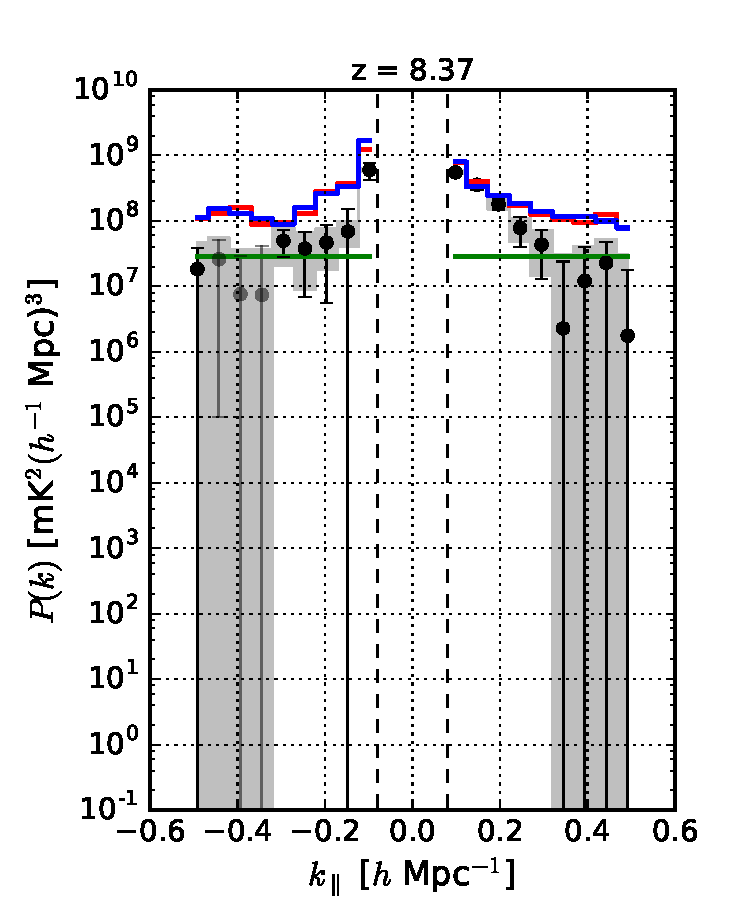
\includegraphics[width=0.45\textwidth]{plots/ps1_data_add.pdf}
	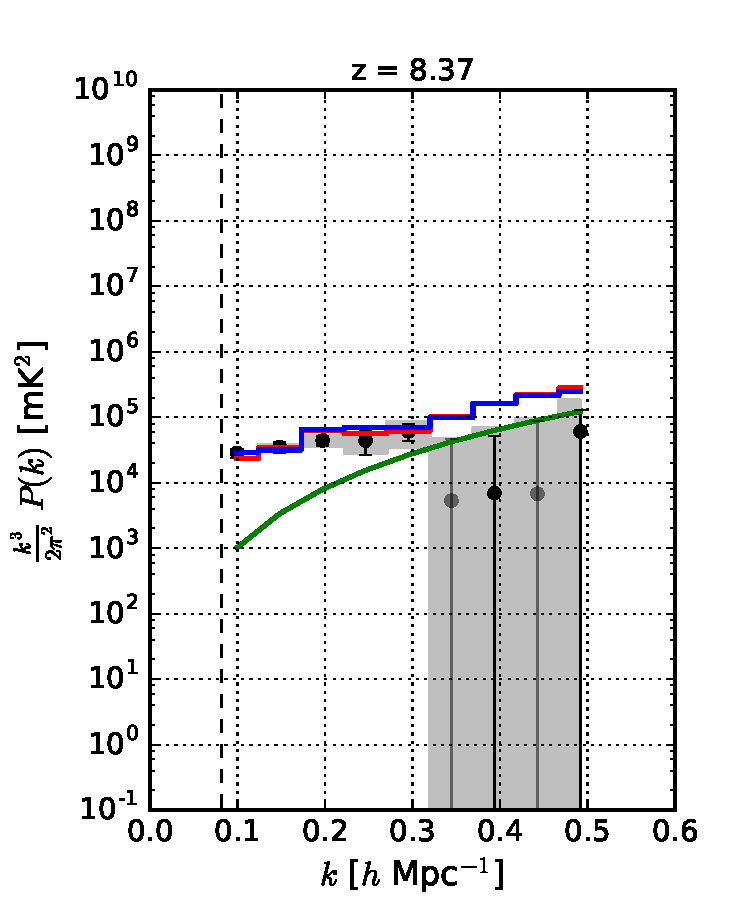
\includegraphics[width=0.45\textwidth]{plots/ps2_data_add.pdf}
	\caption{A power spectrum of a subset of PAPER-64 data illustrating the use of $\widehat{\textbf{C}}_{\rm eff}$ to minimize signal loss. The solid red curve is the $2\sigma$ upper limit on the EoR signal estimated from our signal injection framework. The theoretical $2\sigma$ thermal noise level prediction based on observational parameters is in green. Additionally, the power spectrum result for the uniform weighted case is shown in three different ways: power spectrum values (black and gray points as positive and negative values, respectively, with $2\sigma$ error bars from bootstrapping), the $2\sigma$ upper limit on the EoR signal using our full signal injection framework (solid blue), and the measured power spectrum values with $2\sigma$ thermal noise errors (gray shaded regions). The vertical dashed black lines signify the horizon limit for this analysis using $30$\,m baselines. This power spectrum result does not use the full dataset's sensitivity as in \citet{ali_et_al2015} and Kolopanis et al. (\textit{in prep.}), though we include all analysis changes which have mostly stemmed from revisions regarding signal 
loss, bootstrapping, and the theoretical error computation. We see that the regularization scheme used here produces limits similar to the unweighted limits.}
	\label{fig:ps1_data}
\end{figure*}

In this section we have shown three simple ways of regularizing $\widehat{\textbf{C}}$ to minimize signal loss using PAPER-64 
data. There are many other weighting schemes that we leave for consideration in future work. For example, one could estimate 
$\widehat{\textbf{C}}$ using information from different subsets of baselines. For redundant arrays this might mean calculating $
\widehat{\textbf{C}}$ from a different but similar baseline type, such as the $\sim30$\,m diagonal PAPER baselines (instead of the 
horizontal E/W ones). Alternatively, covariances could be estimated from all baselines except the two being cross-multiplied 
when forming a power spectrum estimate. This method was used in \citet{parsons_et_al2014} (a similar method was also used in \citet{dillon_et_al2015}) in order to avoid suppressing the 
21\,cm signal, and it is worth noting that the PAPER-32 results are likely less impacted from the issue of signal loss underestimation 
because of this very reason (however, they are affected by the error estimation issues described in Chapter \ref{sec:Error}, so 
we also regard those results as suspect and superseded by those of Kolopanis et al. (\textit{in prep.})).

Another possible way to regularize $\widehat{\textbf{C}}$ is to use information from different ranges of LST. For example, one could 
calculate $\widehat{\textbf{C}}$ with data from LSTs where foregrounds are stronger (earlier or later LSTs than the ``foreground-quiet" range typically used in forming power spectra) --- doing so may yield a better description of the foregrounds that we desire to 
down-weight, especially if residual foreground chromaticity is instrumental in origin and stable in time. Fundamentally, each of these examples are similar in that they rely on a computation of $\widehat{\textbf{C}}$ from 
data that is similar but not exactly the same as the data that is being down-weighted. Ideally this would be effective in down-weighting shared contaminants yet avoid signal loss from overfitting EoR modes in the power spectrum dataset itself. 

In Chapter \ref{sec:CaseStudy}, we have detailed several aspects of signal loss in PAPER-64: how the loss arises, how it can be estimated from an injection framework, and ways it can be minimized. We again emphasize that these lessons learned about signal loss are largely responsible for shaping our revised analysis of PAPER data. In the remainder of this paper, we will transition to other aspects of our analysis that have been revised since \citetalias{ali_et_al2015}.

\section{Error Estimation}
\label{sec:Error}

Underestimated signal loss is the main reason for the revision of the power spectrum limits from \citetalias{ali_et_al2015}. It is interesting to note that --- had all the other aspects of the original analysis been correct --- the underestimated limits may have been more easily caught. Unfortunately, two related power spectrum components, namely the error bars on the power spectrum data points and the theoretical noise prediction, were also calculated incorrectly.

In this section, we summarize multiple inconsistencies and errors that have been found since the previous analysis in terms of error estimation. We first describe updated methods regarding bootstrapping, which determines the error bars on our limits. We then highlight an updated calculation for the theoretical noise sensitivity of PAPER-64 and illustrate how our revised calculation has been verified through simulations. 

\subsection{Bootstrapping}
\label{sec:Boot}

Broadly speaking, we desire robust methods for determining accurate 
confidence intervals for our measurements. For PAPER's analysis, we choose a data-driven method of error estimation, computing error bars that have been derived from the inherent 
variance of our measurements. A common technique used to do this is bootstrapping, which we first define below and then discuss its application to PAPER.

Bootstrapping uses sampling with replacement to estimate a posterior distribution. For example, bootstrap measurements (of power spectra, for example) can be made from different random samples of data. Each of these bootstraps is a different realization drawn from some underlying distribution, and realizations are correlated with each other to a degree set by the fraction of sampled points that are held in common between them. Through the process of re-sampling and averaging along different axes of a dataset, such as along baselines or times, we can estimate error bars for our results which represent the underlying distribution of values that are allowed by our measurements (\citealt{efron_tibshirani1994}; \citealt{andrae2010}).

One major caveat of bootstrapping arises when working with correlated data. If, for example, a dataset has many repeated 
values inside it, this would be reflected in each bootstrap. The same value would be present multiple times within a bootstrap 
and also be present between bootstraps, purely because it has a more likely chance of being drawn if there are repeats of 
itself. Therefore, bootstrapping correlated data results in a smaller variation between bootstraps, and hence, underestimates 
errors. 

This is the precisely how errors were underestimated in PAPER-64. Because of fringe-rate filtering, which averages data in time to increase sensitivity, PAPER-64 data is correlated along the time axis. Hence, there are fewer independent samples after filtering, thus decreasing the variance of the bootstraps.

More specifically, the PAPER-64 pipeline outputs $20$ bootstraps (over baselines), each a $2$-dimensional power 
spectrum that is a function of $k$ and time. In \citetalias{ali_et_al2015}, a second round of bootstrapping occurred over the time axis, and a total of $400$ bootstraps were created in this step, each comprised of randomly selected values sampled with replacement (i.e., each of these bootstraps contained the same number of values as the number of time integrations, which, at $\sim$
$700$, greatly exceeds the approximate number of independent samples after fringe-rate filtering).
Means were then taken of the values in each bootstrap. Finally, power 
spectrum limits were computed by taking the mean and standard deviation over all the bootstraps. We emphasize again that in 
this previous analysis, the number of elements sampled per bootstrap greatly 
exceeded the number of independent LST samples, underestimating errors. A random draw of $700$ 
measurements from this dataset has many repeated values, and the variance between hundreds of these random 
samples is smaller than the true underlying variance of the data. 

Given our new understanding of the sensitivity of bootstraps to the number of elements sampled, we have removed the second 
bootstrapping step along time entirely and now simply bootstrap over the baseline axis. Power spectrum $2\sigma$ errors (computed from bootstrap variances) with and without this bootstrapping change for a fringe-rate filtered noise simulation are shown in Figure 
\ref{fig:data_errors} in black and gray, respectively. The estimates are uniformly weighted in order to disentangle the effects of bootstrapping from signal loss. As 
shown in the figure, when more elements are drawn for each bootstrap than the number of 
independent samples (by over-sampling elements along the time axis), repeated values begin to crop up and the apparent variation between bootstraps drops, resulting in limits (gray) below the predicted noise level (green). Using the revised bootstrapping method, where bootstrapping only occurs over the baseline axis, the limits (black) are shown to agree with the analytic prediction for noise. While Figure \ref{fig:data_errors} implies that errors, computed prior to our bootstrapping change (gray), are underestimated by a factor of $\sim$ $5$ in mK$^{2}$ for the noise simulation (whose creation details are outlined in the next section), in practice this factor is lower for the case of real data (a factor of $\sim$ $3$ in mK$^{2}$ instead), possibly due to the data being less correlated in time than the fringe-rate filtered noise in the simulation. 

In addition to learning how sample independence affects bootstrapped errors, we have made three additional changes to our bootstrapping procedure since \citetalias{ali_et_al2015}, summarized here:

\begin{itemize}

\item{A second change to our bootstrapping procedure is that we now bootstrap over baseline cross-products, instead of the baselines themselves. In the previous analysis, baselines were bootstrapped prior to forming cross power spectra, and using this particular ordering of operations (bootstrapping, then cross-multiplication) yields variances that have been found to disagree with predicted errors from bootstrapping using simulations. On the contrary, bootstrapping over cross power spectra ensures that we are estimating the variance of our quantity of interest (i.e., the power spectrum). This change, while fundamental in retaining the integrity of the bootstrapping method in general, alters the resulting power spectrum errors by factors of $<2$ in practice.}

\item{In \citetalias{ali_et_al2015}, individual baselines were divided into five independent groups, where no baselines were repeated in each group. Then, baselines within each group were averaged together, and the groups were cross-multiplied to form power spectra. This grouping method was used to reduce computational time, however upon closer examination it has been found that the initial grouping introduces an element of randomness into the final measurements --- more specifically, the power spectrum value fluctuates depending on how baselines are assigned into their initial groups. Our new approach removes this element of randomness at the cost of computational expense, as we now perform all baseline cross-products.}

\item{Finally, the last change from the \citetalias{ali_et_al2015} method is that our power spectrum points (previously computed as the mean of all bootstraps), are now computed as the power spectrum estimate resulting from not bootstrapping at all. More specifically, we compute one estimate without sampling, and this estimate is propagated through our signal loss computation (this estimate is $\widehat{\textbf{P}}_{x}$). The difference between taking the mean of the bootstrapped values and using the estimate from the no-bootstrapping case is small, but doing the latter ensures that we are forming results that reflect the estimate preferred by all our data.}

\end{itemize}

In summary, we have learned several lessons regarding bootstrapping and have revised our analysis procedure in order to determine error bars that correctly reflect the variance in our power spectrum estimates. Bootstrapping can be an effective and straightforward way to estimate errors of a dataset, however, bootstrapping as a means of estimating power spectrum errors from real fringe-rate filtered data requires knowledge of the number of independent samples, which is not always a trivial task. We have thus avoided this issue by removing one of our bootstrap axes, as well as updated several other details of our procedure to ensure accurate re-sampling and error estimation.

\begin{figure}
	\centering
	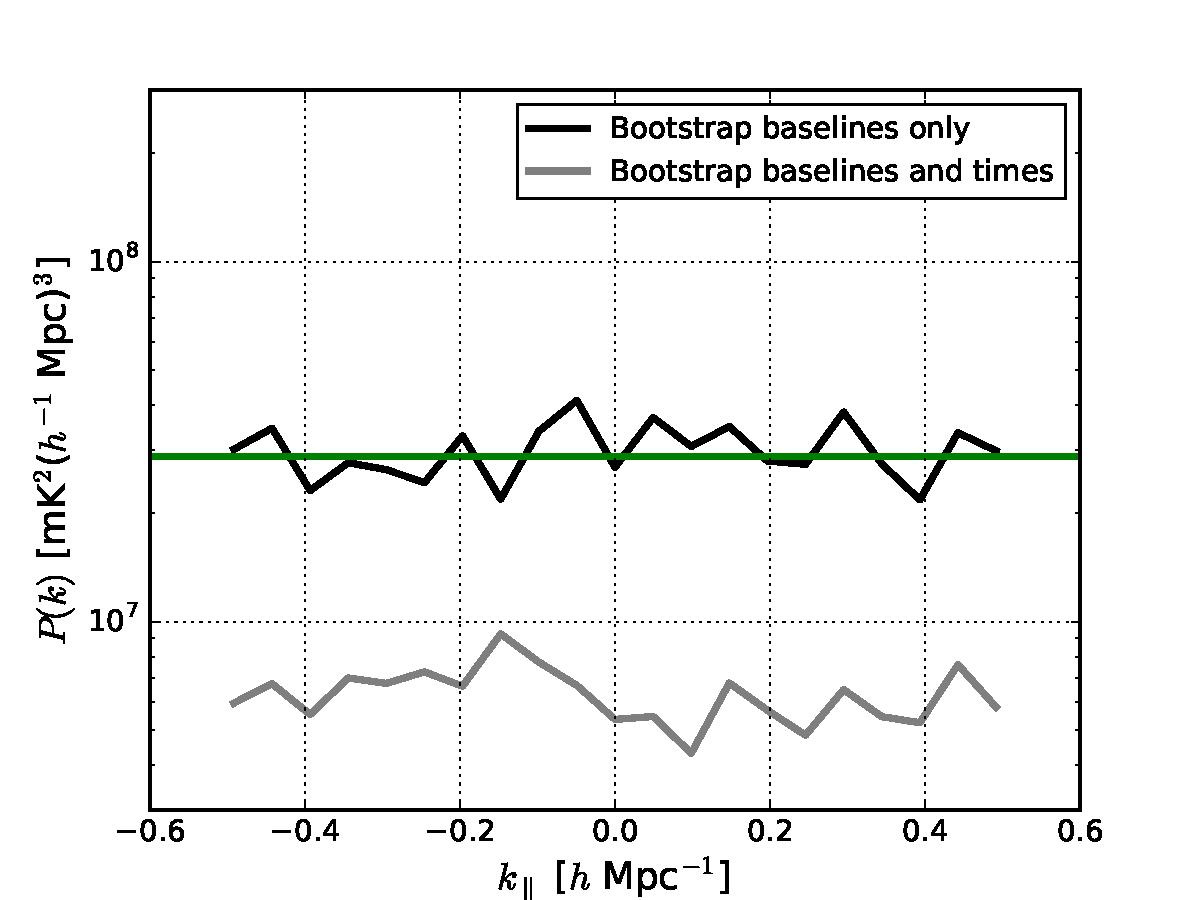
\includegraphics[trim={0.3cm 0cm 0.3cm 0.3cm},width=0.8\textwidth]{plots/noise_errors.pdf}
	\caption{$2\sigma$ power spectrum errors (from bootstrap variances) for a noise simulation (computed via Equation \eqref{eq:noise} using PAPER-64 observing parameters) using two different bootstrapping 
methods. The noise is fringe-rate filtered and a weighting matrix of $\textbf{I}$ (uniform-weighted) is used in order to disentangle the 
effects of bootstrapping from signal loss. The bootstrapping method used in \citet{ali_et_al2015} is shown in gray, where bootstrapping occurs along both the baseline and time axes. This underestimates errors by sampling more values than independent ones in the dataset (fringe-rate filtering reduces the number of independent samples along time). We use the method illustrated by the black curve in our updated analysis, where bootstrapping only occurs along the baseline axis. We find that these revised limits agree with the $2\sigma$ analytic prediction for noise (green).}
	\label{fig:data_errors}
\end{figure}

\subsection{Theoretical Error Estimation}
\label{sec:Error}

One useful way of cross-checking measured power spectrum values and errors is to compute a theoretical estimation of thermal noise based on observational parameters. Although a theoretical model often differs from true errors, it is helpful to understand the ideal case and the factors that affect its sensitivity. Upon re-analysis of PAPER-64, we have discovered that this estimate was also underestimated in previous analyses. 

To compute our theoretical noise estimate, we use an analytic sensitivity calculation. Through detailed studies using several independently generated noise simulations, what we found was that our simulations all agreed but were discrepant with the previous calculations. The analytic 
calculation is only an approximation and attempts to combine a large number of pieces of information in an approximate way; however, when re-considering some of the approximations, the differences were large enough (factors of $10$ in some cases) to warrant a 
careful investigation. What follows here is an 
accounting of the differences which have been discovered. We note that our theoretical error estimate, which is plotted as the solid green curve in many of the previous power spectrum plots in this paper, is computed with these changes accounted for.

The noise prediction $n(k)$ (\citealt{parsons_et_al2012a}; \citealt{pober_et_al2013}) for a power spectral analysis of 
interferometric 21\,cm data, in temperature-units, is:

\begin{equation}
\label{eq:sense}
N(k) = \frac{X^{2}Y \Omega_{\rm eff} T_{\rm sys}^{2}}{\sqrt{2N_{\rm lst}N_{\rm seps}}\,t_{\rm int}N_{\rm days}N_{\rm bls}N_{\rm pols}}.
\end{equation}
We will now explain each factor in Equation \eqref{eq:sense} and highlight key differences from the numbers used in \citetalias{ali_et_al2015}.

\begin{itemize}
\item $X^{2}Y$: Conversion factors from observing coordinates (angles on the sky and frequency) to cosmological coordinates (co-moving 
distances). For $z=8.4$, $X^{2}Y = 5 \times 10^{11} \, h^{-3}$ Mpc$^{3}$ str$^{-1}$ GHz$^{-1}$.
\item $\Omega_{\rm eff}$: The effective primary beam area in steradians (\citealt{parsons_et_al2010}; \citealt{pober_et_al2012}). 
The effective beam area changes with the application of a fringe-rate filter, since different parts of the beam are up-weighted and down-weighted. Using numbers from Table 1 in \citet{parsons_et_al2016}, $\Omega_{\rm eff} = 0.74^{2}/0.24$ for an optimal fringe-rate 
filter and the PAPER primary beam. 
\item $T_{\rm sys}$: The system temperature is set by:

\begin{equation}
\label{eq:sys}
T_{\rm sys} = 180\Big(\frac{\nu}{0.18}\Big)^{-2.55} + T_{\rm rcvr},
\end{equation}

where $\nu$ are frequencies in GHz (\citealt{thompson_et_al2001}). We use a receiver temperature of $144$\,K, yielding $T_{\rm sys} = 431$\,K at $150$\,MHz. 
This is lower than the $T_{\rm sys}$ of $500$\,K used in \citetalias{ali_et_al2015} because of several small miscalculation errors that were 
identified\footnote{For example, there was a missing a square root in going from a variance to a standard deviation.}.
\item $\sqrt{2}$: This factor in the denominator of the sensitivity equation comes from taking the real part of the power spectrum 
estimates after cross-multiplying two independent visibility measurements. In \citetalias{ali_et_al2015}, a factor of $2$ was mistakenly used.
\item $N_{\rm lst}$: The number of independent LST bins that go into a power spectrum estimation. The sensitivity scales as the square root 
because we integrate incoherently over time. For PAPER-64, $N_{\rm lst} = 8$.
\item $N_{\rm seps}$: The number of baseline separation types (where baselines of a unique separation type have the same orientation and length) averaged incoherently in a final power spectrum estimate. For the 
analysis in this paper, we only use one type of baseline (PAPER's 30\,m East/West baselines). However, both the updated limits in Kolopanis et al. (\textit{in prep.}) and the sensitivity prediction in Figure \ref{fig:sense_check} use three separation types ($N_{\rm seps}=3$) to match \citetalias{ali_et_al2015}.
\item $t_{\rm int}$: Length of an independent integration of the data. It is crucial to adapt this number if filtering is applied along the time axis (i.e., a 
fringe-rate filter). We compute the effective integration time of our fringe-rate filtered data by scaling the original integration time $t_{i}$
using the following:
\begin{equation}
t_{\rm int} = t_{i} \frac{\int1 \, df}{\int w^{2}(f) \,df},
\end{equation}
where $t_{i}=43$ seconds, $t_{\rm int}$ is the fringe-rate filtered integration time, $w$ is the fringe-rate profile, and the integral is 
taken over all fringe-rates. For PAPER-64, this number is $t_{\rm int} = 3857$\,s. 
\item $N_{\rm days}$: The total number of days of data analyzed. In \citetalias{ali_et_al2015}, this number was set to $135$. However, because we 
divide our data in half (to form ``even" and ``odd" datasets, or $N_{\rm datasets} = 2$), this number should reflect the number of days in each individual dataset instead of the total. Additionally, this number should be adjusted to reflect the actual number of cross-multiplications that occur between datasets (``even" with ``odd" and ``odd" with ``even", but not ``odd" with ``odd" or ``even" with ``even" in order to avoid noise biases). Finally, because our LST coverage is not $100\%$ complete (it doesn't overlap for every single day), we incorporate a root-mean-square statistic in computing a realistic value of 
$N_{\rm days}$. Our expression therefore becomes:
\begin{equation}
N_{\rm days} = \sqrt{\langle N_{i}^{2}\rangle} \sqrt{(N_{\rm datasets}^{2}-N_{\rm datasets})}
 %\frac{1}{N_{\rm days}} = \sqrt{\Big\langle\frac{1}{N_{i}^{2}} \Big\rangle_{i}},
 \end{equation}
\noindent where $i$ indexes LST and frequency channel over all datasets (\citealt{jacobs_et_al2015}). For PAPER-64, our revised estimate of $N_{\rm days}$ is $\sim47$ 
days.
\item $N_{\rm bls}$: The number of baselines contributing to the sensitivity of a power spectrum estimate. In \citetalias{ali_et_al2015}, this number was 
the total number of $30$\,m East/West baselines used in the analysis. However, using the total number of baselines ($N_{\rm bls\_total} = 51$) neglects 
the fact that the \citetalias{ali_et_al2015} analysis averages baselines into groups for computational speed-up when cross-multiplying data. Our revised estimate for the parameter is:
\begin{equation}
N_{\rm bls} = \frac{N_{\rm bls\_total}}{N_{\rm gps}}\sqrt{\frac{N_{\rm gps}^{2}-N_{\rm gps}}{2}},
\end{equation}
\noindent where, in the \citetalias{ali_et_al2015} analysis, $N_{\rm gps} = 5$. Each baseline group averages down linearly as the number of baselines 
entering the group ($N_{\rm bls\_total}/N_{\rm gps}$) and then as the square root of the number of cross-multiplied pairs \Big($\sqrt{\frac{N_{\rm gps}^{2} - 
N_{\rm gps}}{2}}$\Big). A revised \citetalias{ali_et_al2015} analysis should therefore use $N_{\rm bls} \sim 32$ instead of $51$, and this change is taken into account in Figure \ref{fig:sense_check}. However, the analysis in this paper and in Kolopanis et al. (\textit{in prep.}) no longer averages baselines into groups ($N_{\rm gps} = 1$). For the subset of data presented in this paper, $N_{\rm bls} = 10$.
\item $N_{\rm pols}$: The number of polarizations averaged together. For the case of Stokes I, $N_{\rm pols}=2$.
\end{itemize}

An additional factor of $\sqrt{2}$ is gained in sensitivity when folding together positive and negative $k$'s to form $\Delta^{2}(k)$.

Our revised sensitivity estimate for the \citetalias{ali_et_al2015} analysis of PAPER-64 is shown in Figure \ref{fig:sense_check}. 
Together, the revised parameters yield a decrease in sensitivity (higher noise floor) by a factor of $\sim7$ in mK$^{2}$. 

\begin{figure}
	\centering
	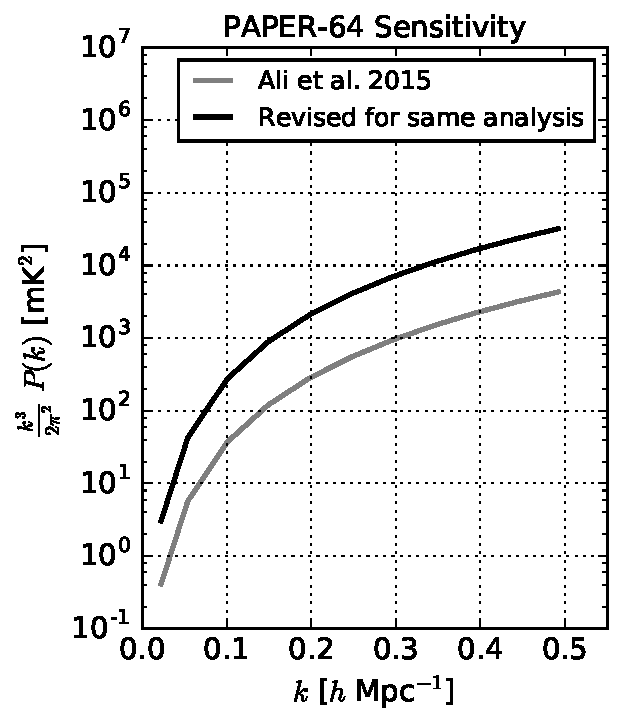
\includegraphics[width=0.55\textwidth]{plots/sense_check.pdf}
	\caption{An updated prediction for the thermal noise level of PAPER-64 data (black) is shown in comparison to previously 
published sensitivity limits (gray), both computed for the parameters and methods used in \citet{ali_et_al2015}. Major factors that contribute to the discrepancy are $
\Omega_{\rm eff}$, $N_{\rm days}$ and $N_{\rm bls}$, as in Equation \eqref{eq:sense} and described in Chapter \ref{sec:Error}, which when combined decreases our 
sensitivity (higher noise floor) by a factor of $\sim7$ in mK$^{2}$.}
	\label{fig:sense_check}
\end{figure}

To verify our thermal noise prediction, we form power spectra estimates using a pure noise simulation. We create Gaussian 
random noise assuming a constant $T_{\rm rcvr}$ (translated into $T_{\rm sys}$ via Equation \eqref{eq:sys}) but accounting for the true $N_{\rm days}$ as determined 
by LST sampling counts for each time and frequency in the LST-binned data. We convert $T_{\rm sys}$ into a root-mean-square variance statistic 
using:

\begin{equation}
\label{eq:noise}
T_{\rm rms} = \frac{T_{\rm sys}}{\sqrt{\Delta\nu \Delta t N_{\rm days} N_{\rm pols}}},
\end{equation}

\noindent where $\Delta\nu$ is the channel spacing, $\Delta t$ is the integration time, $N_{\rm days}$ is the number of daily counts for a 
particular time and frequency that went into our LST-binned set, and $N_{\rm pols}$ is the number of polarizations ($2$ for Stokes 
I). This temperature sets the variance of the Gaussian random noise.

Power spectrum results for the noise simulation, which uses our full power spectrum pipeline, are shown in Figure 
\ref{fig:ps_noise}. We highlight that the bootstrapped data (black and gray points, with $2\sigma$ error bars) and thermal noise prediction (solid green) show good agreement, as bootstrapping provides an accurate estimate of the noise variance. However, the limits from the full signal loss framework (weighted and unweighted in red and blue, respectively) are inflated, likely due to the additional inclusion of sample variance that comes from the EoR simulations. While the noise simulation provides an important indicator about the accuracy of our theoretical noise calculation, we note that the calculation did not take into account additional sources of error associated with earlier analysis steps (for example, \citet{trott_wayth_2017} show how calibration specifically can add errors to visibilities). Additionally, we recommend that future work investigate possible error correlations between baseline pairs and any interaction effects between signal and noise that may effect error calculations. Because of these reasons, we therefore interpret our noise prediction as the sensitivity floor for our measurements.

\begin{figure*}
	\centering
	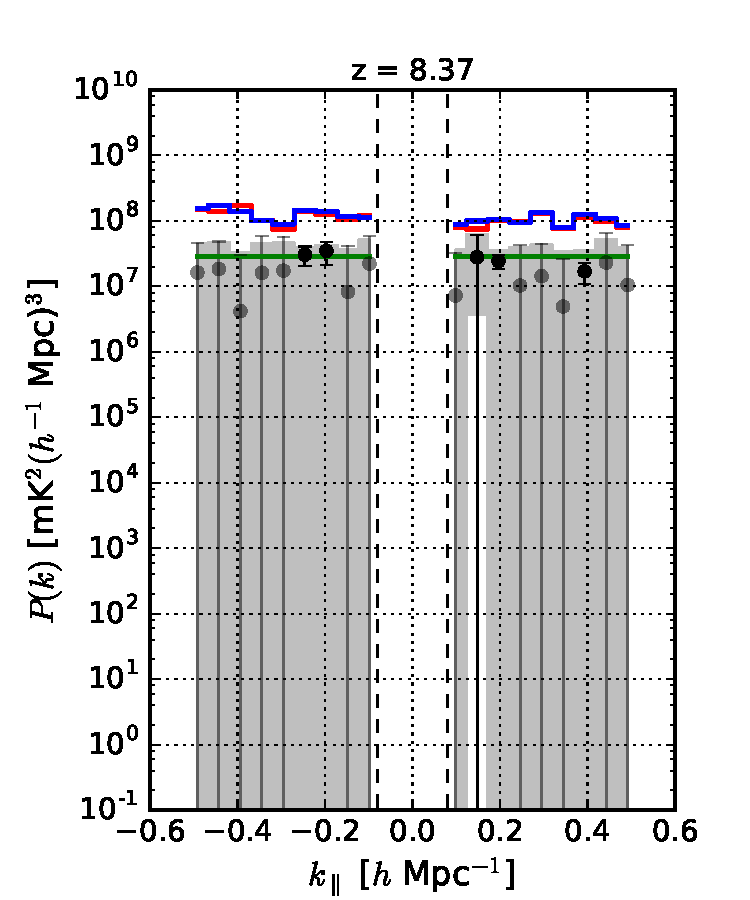
\includegraphics[width=0.45\textwidth]{plots/ps1_noise_add.pdf}
	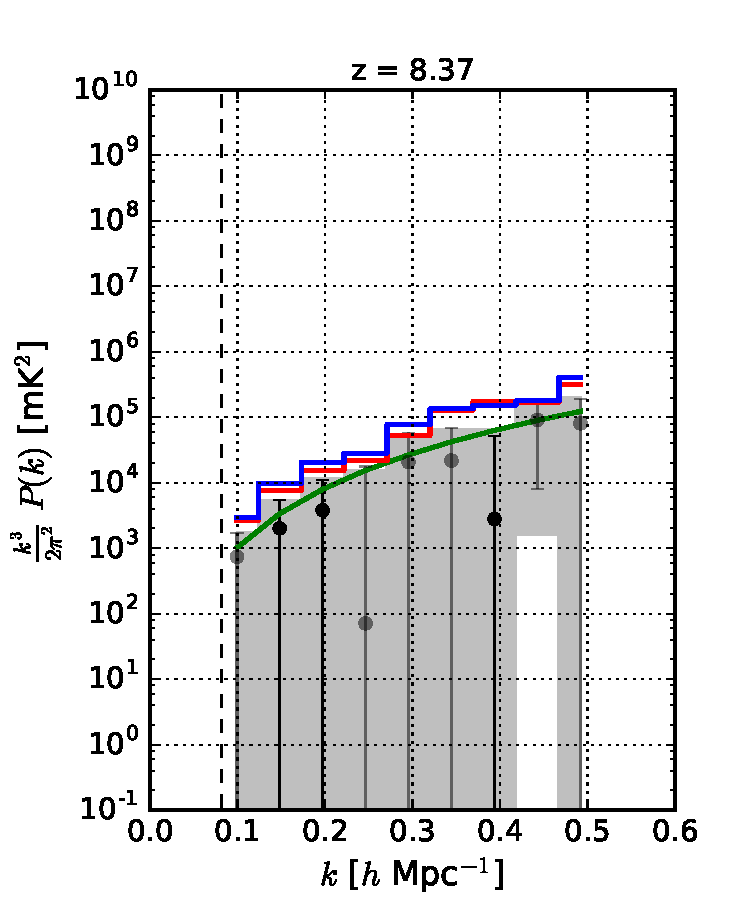
\includegraphics[width=0.45\textwidth]{plots/ps2_noise_add.pdf}
	\caption{The power spectrum for a noise simulation that mimics the noise level of a subset of PAPER-64 data, where the solid red curve is the $2\sigma$ upper limit on the EoR signal estimated from our signal injection framework using $\widehat{\textbf{C}}_{\rm eff}$. The theoretical $2\sigma$ thermal noise level prediction based on observational parameters (calculated by Equation \eqref{eq:sense}) is in green. Additionally, the power spectrum result for the uniform weighted case is shown in three different ways: power spectrum values (black and gray points as positive and negative values, respectively, with $2\sigma$ error bars from bootstrapping), the $2\sigma$ upper limit on the EoR signal using our full signal injection framework (solid blue), and the measured power spectrum values with $2\sigma$ thermal noise errors (gray shaded regions). The vertical dashed black lines signify the horizon limit for this analysis using $30$\,m baselines. We highlight that the bootstrapped data points and thermal noise prediction show good agreement, while the limits from the full injection framework (red and blue) are inflated due to the additional inclusion of sample variance that comes from the injection simulations.}
	\label{fig:ps_noise}
\end{figure*}

\section{Bias}
\label{sec:Bias}

In Chapter \ref{sec:BiasOverview} we highlighted some common sources of bias that can show up as power spectrum 
detections and imitate an EoR signal. We discussed the importance of using jackknife and null tests for instilling confidence in an EoR 
detection, as well as for identifying other sources of biases. Here we demonstrate methods used by PAPER-64 to mitigate 
foreground and noise bias and we perform null tests in order to characterize the stability and implications of our results.

\subsection{Mitigating Bias}
\label{sec:MitBias}

We briefly discuss one way we mitigate foreground leakage in a power spectrum estimate, and two ways we 
suppress noise biases. These methods are not novel to this analysis but here we frame them in the context of minimizing false 
(non-EoR) detections. 

Tailoring window functions is one way to suppress foreground biases (similar discussions to the following one are in \citet{liu_et_al2014b} and \citetalias{ali_et_al2015}). As alluded to in Chapter \ref{sec:SiglossOverview}, we 
have a choice for the normalization matrix $\textbf{M}$ in Equation \eqref{eq:phat}. For the analysis of PAPER-64 data, we 
compute $\textbf{M}$ using the matrix $\textbf{G}$ (which would be the Fisher matrix if $\textbf{R} \equiv \textbf{C}^{-1}$), defined as:

\begin{equation}
\textbf{G}^{\alpha\beta} = \frac{1}{2} \text{tr} [\textbf{R}\textbf{Q}^{\alpha}\textbf{R}\textbf{Q}^{\beta} ]
\end{equation}

\noindent where $\textbf{R}$ is the data-weighting matrix and $\alpha$ and $\beta$ are wavebands in $k_{\parallel}$. We take 
the Cholesky decomposition of $\textbf{G}$, decomposing it into two lower triangular matrices (which is possible since $\textbf{G}$ is Hermitian):

\begin{equation}
\textbf{G} = \textbf{LL}^{\dagger}.
\end{equation}

\noindent Next, we construct $\textbf{M}$:

\begin{equation}
\textbf{M} = \textbf{DL}^{-1}
\end{equation}

\noindent where $\textbf{D}$ is a diagonal matrix. In doing so, our window function, defined as $\textbf{W} = \textbf{MG}$ (see Equation \eqref{eq:Wpplusbias}), 
becomes

\begin{equation}
\textbf{W} = \textbf{DL}^{\dagger}.
\end{equation}

\noindent Because of the nature of the lower triangular matrix, this window function has the property of preventing the leakage 
of foreground power from low-$k$ to high-$k$ modes. Specifically, we order the elements in $\textbf{G}$ in such a way so that 
power can leak from high-$k$ modes to low-$k$ modes, but not vice versa. Since most foreground power shows up at low-$k$'s, this method ensures a window function that retains clean, noise-dominated measurements while minimizing the 
contamination of foreground bias. This tailored window function was used in the \citetalias{ali_et_al2015} analysis, however throughout this paper, we use a diagonal $\textbf{M}$ for simplicity.

In addition to mitigating foreground bias at high-$k$'s, two other sources of bias that we actively suppress in the PAPER-64 
analysis are noise bias associated with the squaring of thermal noise and noise bias from crosstalk. In order to avoid the 
former, we filter out certain cross-multiplications when forming $\widehat{q}$ in Equation \eqref{eq:qhat}. Namely, the PAPER-64 
dataset is divided into two halves: even Julian dates and odd Julian dates. Our data vectors are then $\textbf{x}_{even, 1}$ for 
the ``even" dataset and baseline $1$, $\textbf{x}_{odd, 1}$ for the ``odd" dataset and baseline $1$, etc. We only form 
$\widehat{q}$ when the two copies of $\textbf{x}$ come from different groups and baselines, never multiplying ``baseline 1" with ``baseline 1", for 
example, in order to prevent the squaring of the same thermal noise. 

To mitigate crosstalk bias, which appears as a static bias in time, we apply a fringe-rate filter that suppresses fringe-rates of 
zero. Figure \ref{fig:frp} shows that the filter response is zero for such static signals. The effect of filtering out zero fringe-rates 
on power spectrum results is shown in \citetalias{ali_et_al2015}. Most notably, even without accounting for signal loss, the crosstalk bias at all $k$'s is very strong compared to the removed case.

\subsection{Jackknife/Null Tests}

As shown in Figure \ref{fig:ps1_data}, our illustrative PAPER-64 power spectrum shows biases above the predicted noise level, particularly at low-$k$ values. As discussed in Chapter \ref{sec:BiasTypes}, this bias is
most likely attributable to foreground leakage. %The cause for biases at higher $k$-values is more difficult to pinpoint. 

Here we perform three null tests on PAPER-64 data that aim to isolate systematics in the data and verify 
that our biases are not attributable to EoR. Similar to in Chapter \ref{sec:JackknifeOverview}, we take jackknives along different axes of the dataset to produce multiple power spectra. We then difference them (i.e., the null test) to tease out excess variances.

The three results are shown in Figure \ref{fig:null}. Each test displays the differenced power spectrum between two halves of a jackknife, where the plotted points are the differenced power spectrum values, and the plotted errors are the bootstrapped errors of the two dataset halves added in quadrature. The expected thermal noise level (gray shaded regions) is the thermal noise of each dataset added in quadrature as well. Constructing the tests as such ensures that we are probing whether the variances of each dataset differ by an amount consistent with the thermal noise. We use uniform weightings for all tests. 

We take jackknives along three different axes:

\begin{itemize}
%\item Original Data (black): This is identical to the unweighted, revised PAPER-64 power spectrum in Figure \ref{fig:ps1_data} (one baseline type only) with weighting matrix $\textbf{I}$. There are clear detections at low $k$'s.
\item Baselines: We split our dataset into two halves, where each contains half of the total baselines used in the 
analysis. No baselines are repeated between the two datasets.
\item Sidereal Hour: We split our dataset into two halves based on LST, namely the first half (LSTs 0.5-4.5 hours) and second half (LSTs 
4.5-8.6 hours).
\item Day: We split our dataset into even and odd Julian dates. We form power spectra for each separately, allowing the cross-multiplication of ``even" with ``even", for example, for this null test only. If the same sky signal is in both the ``even" and ``odd" datasets, we expect it to cancel out. %However, allowing these cross-multiplications can in practice introduce a low level noise bias... 
\end{itemize}

\begin{figure*}
	\centering
	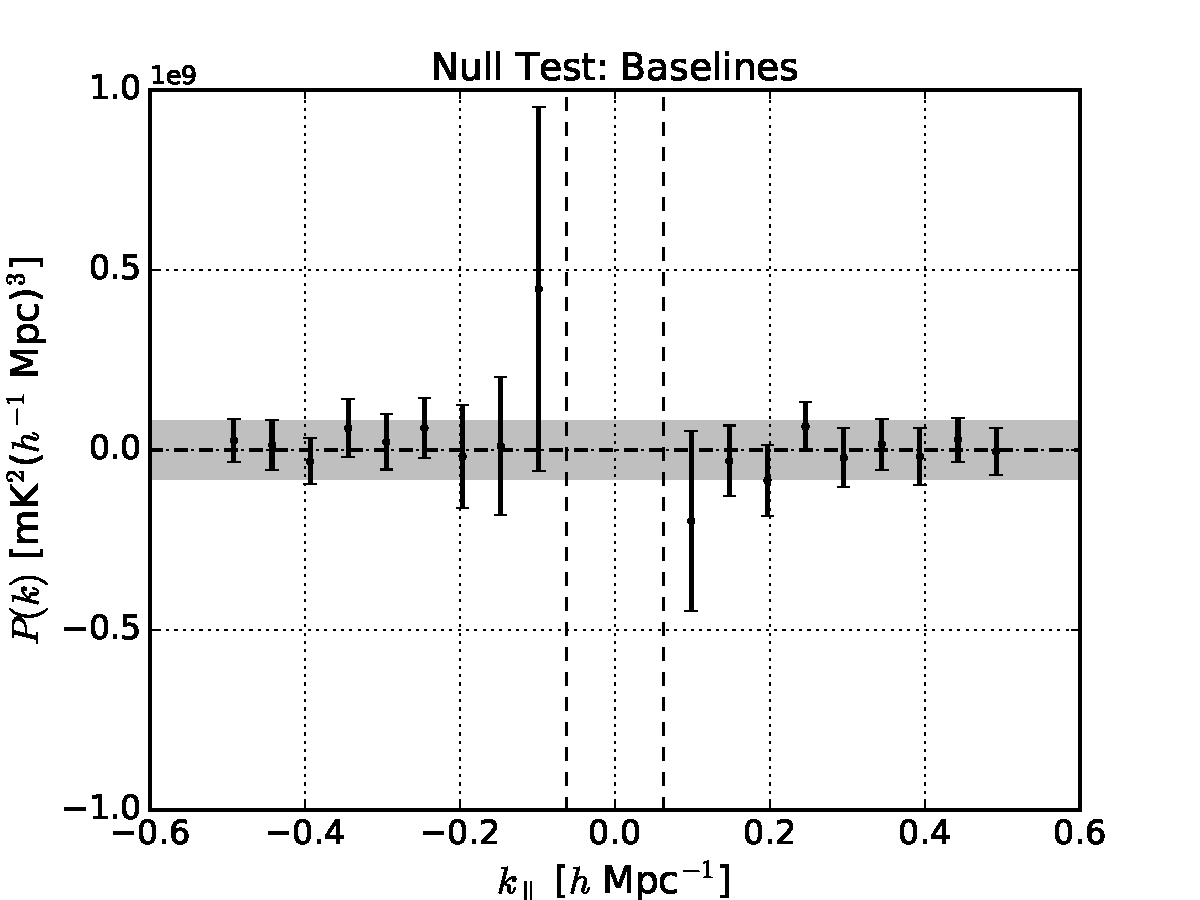
\includegraphics[width=0.47\textwidth]{plots/null_bls.pdf}
	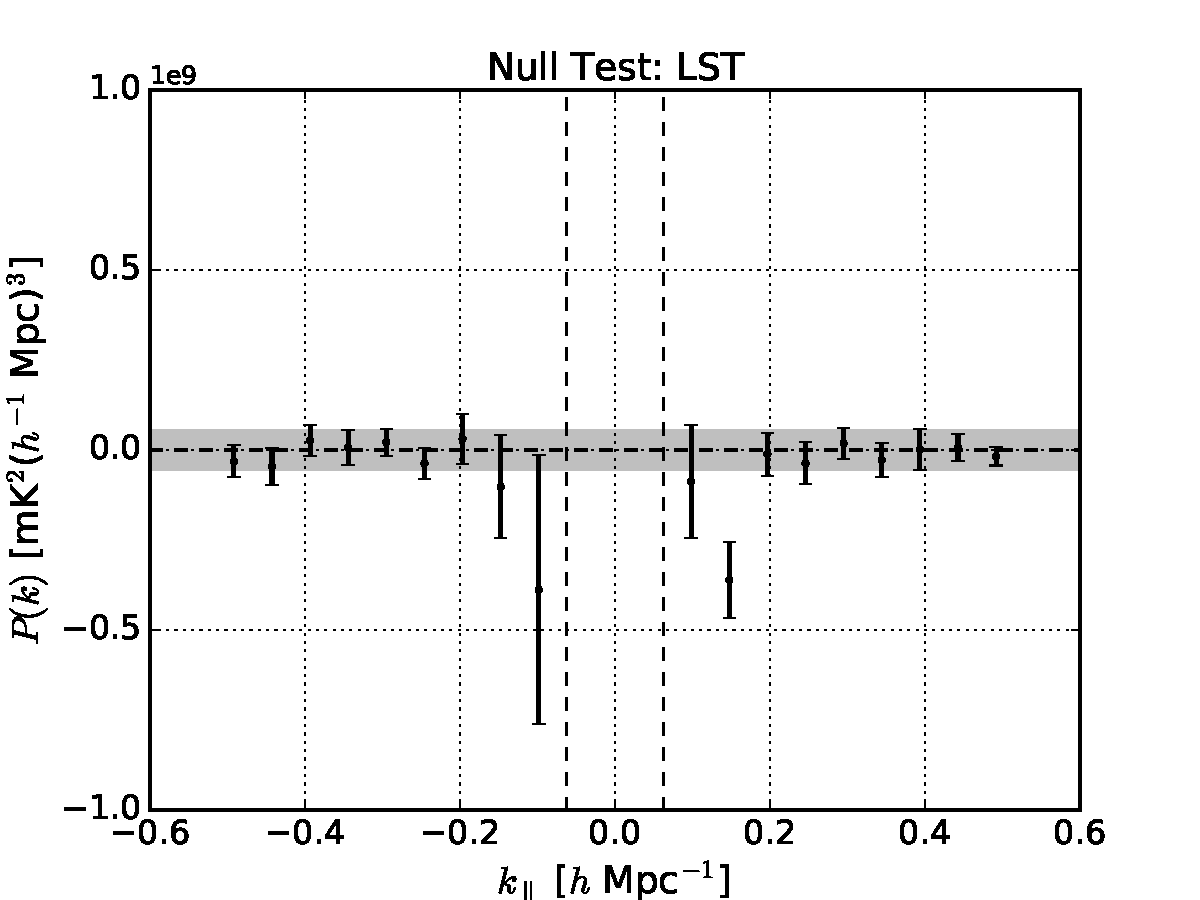
\includegraphics[width=0.47\textwidth]{plots/null_lsts.pdf}
	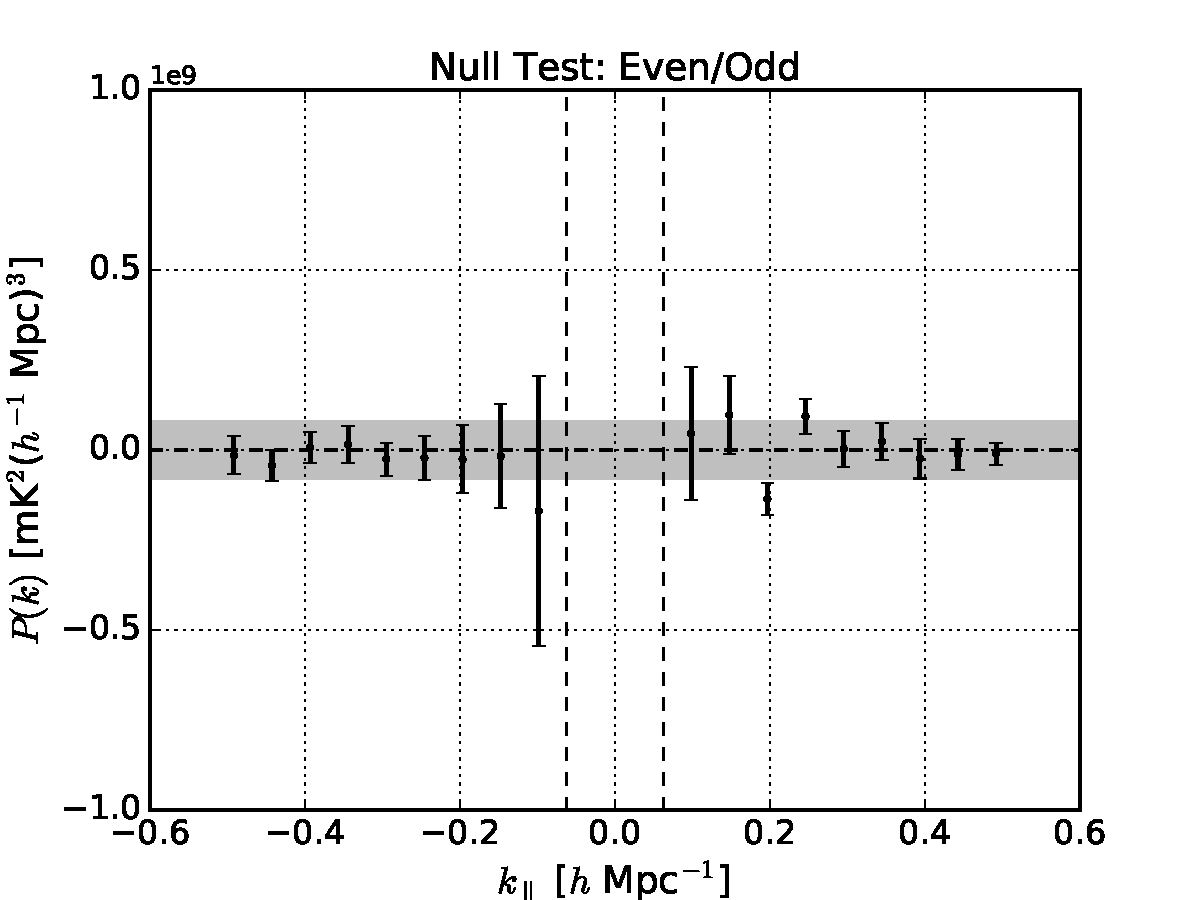
\includegraphics[width=0.47\textwidth]{plots/null_eo.pdf}
	\caption{Differenced power spectrum results (with $2\sigma$ bootstrapped errors) for three null tests, where a jackknife is taken along the baseline axis (top left), LST axis (top right), and even/odd Julian date axis (bottom). The results shown are unweighted (no signal loss), where the power spectrum values plotted are computed from the difference between two power spectra produced on either side of the jackknife axis. The gray shaded region in each plot is the estimated $2\sigma$ theoretical noise limit given the parameters of each test. We find that there are no significant systematics for $k > \pm 0.2$\,$h$ Mpc$^{-1}$ for all three tests. However, we find that all tests exhibit an extra variance at $k$-values near the horizon ($k\sim\pm 0.1$\,$h$ Mpc$^{-1}$), likely due to foreground-noise coupling terms when foregrounds are brightest. Additionally, we find that the LST null test is not fully consistent with zero, implying a bias that is LST dependent and likely caused by varying foregrounds.}
	\label{fig:null}
\end{figure*}

In investigating Figure \ref{fig:null}, we focus on three main possibilities --- whether the data points and error bars are consistent with thermal noise (``passing"), whether the error bars are consistent with zero but not consistent with thermal noise (``passing but has an additional variance"), or whether the error bars are not consistent with zero at all (``failing"). We examine each case in the context of our results below.

Firstly, all three null tests display data points that lie within the thermal noise gray band for $k > \pm 0.25$\,$h$ Mpc$^{-1}$. In addition, all three null tests show error bars consistent with the thermal noise level for those same $k$'s. This implies that the two jackknife halves do not differ by an amount greater than the thermal noise (i.e., the baselines making up the two jackknives either do not contain bias, or contain similar amounts of bias; we suspect it is the former though more thorough jackknives along this axis are needed to make this conclusion). We deem these as ``passing" null tests for the specific jackknives taken (again, dividing up the data in a different way along the same axes may not yield the same results, so more thorough testing is needed to be sure).

The second null test possibility (error bars consistent with zero but not with thermal noise) is displayed by the $k$-values just outside the horizon ($k\sim\pm 0.1$\,$h$ Mpc$^{-1}$) for all three tests. This indicates an additive noise component that is increasing our errors. More specifically, although we expect each cross-multiplication that is used in power spectrum estimation to have independent noise, there is still the possibility of a noise-foreground coupling term that can introduce power. This is because cross-multiplications produce four additive terms --- a signal-squared term (where ``signal" includes both foregrounds and EoR), two cross-terms between the signal and noise, and one noise-only term. When differencing two power spectra (each with their own four terms), we expect the signal-only term to subtract out for a ``passing" null test, and we expect the noise-only terms to be consistent with thermal noise. While the cross-terms have a mathematical expectation value of zero, in practice we are limited by our number of samples ($90$ cross-products for this analysis times $\sim$ $8$ independent LST samples). Combined with the fact that the foregrounds are so bright, the finite ensemble of the couplings can introduce extra variance that varies with foreground strength. It is therefore not surprising that this effect is largest at $k$-values just outside the horizon, where we expect foregrounds to be brightest post-delay filtering.

Lastly, a third null test result is an error bar not consistent with zero. This is the case for the LST null test at $k\sim-0.1$\,$h$ Mpc$^{-1}$ and $k\sim0.15$\,$h$ Mpc$^{-1}$, as well as the even/odd test at $k\sim0.2$\,$h$ Mpc$^{-1}$ and $k\sim0.25$\,$h$ Mpc$^{-1}$. In such a case, the two jackknife halves differ by an amount greater than the thermal noise (i.e., the data point is not in the thermal noise band), yet they are each constrained tightly by individual error bars that when combined, are not consistent with zero. This result implies that there exists a low level bias that is LST-dependent and Julian date-dependent. The former is likely caused by residual foregrounds that vary in LST, and it is not surprising that this type of bias occurs near the horizon limit. The latter requires further investigation that we leave to future work.

In this section we have presented the first jackknife and null tests from the PAPER experiment. Unsurprisingly, they imply that our measurements are biased by foregrounds, and not the EoR signal (a clean detection of EoR would have passed all three tests). While simple, these tests outline a framework that can be used by future measurements. The 21\,cm community is beginning to recognize the importance of these types of tests (\citealt{pober_et_al2016b}) in characterizing power spectra at the EoR level, and it is clear that future results will require more substantial and thorough investigations of this nature.

\section{Summary}

Although current 21\,cm published power spectrum upper limits lie several orders of magnitude above predicted EoR levels, 
ongoing analyses of deeper sensitivity datasets from PAPER, MWA, and LOFAR, as well as next generation instruments like 
HERA, are expected to continue to push towards EoR sensitivities. As the field progresses towards a detection, we have shown 
that it is crucial for future analyses to have a rigorous understanding of signal loss in an analysis pipeline and be able to accurately 
and robustly calculate both power spectrum and theoretical errors.

In particular, in Chapters \ref{c.PSmethods} and \ref{c.PSA64} we have investigated the subtleties and tradeoffs of common 21\,cm power spectrum techniques on 
signal loss and error estimation, which can be summarized as follows:

\begin{itemize}
\item Substantial signal loss can result when weighting data using empirically estimated covariances due to couplings with the data realizations (Chapter 
\ref{sec:SiglossOverview}). Loss of the 21\,cm signal is especially significant the fewer number of independent modes that
exist in the data. Hence, there exists a trade-off between sensitivity driven 
time-averaging techniques such as fringe-rate filtering and signal loss when using empirically estimated covariances. 
\item Signal injection and recovery simulations can be used to quantify signal loss (Chapter \ref{sec:siglossmethod}). However, a 
signal-only simulation (i.e., comparing a uniformly weighted vs. weighted power spectrum of EoR only) can underestimate loss by 
failing to account for correlations between the data and signal which can be large and negative.
\item Errors that are estimated via bootstrapping can be underestimated if samples in the dataset are significantly correlated 
(Chapter \ref{sec:Boot}). However, if the number of independent samples in a dataset is well-determined, bootstrapping is a 
simple and accurate way of estimating errors.
\end{itemize}

As a consequence of our investigations, we have also used a subset of PAPER-64 data to make a new power spectrum analysis. This serves as an illustrative example of using a signal injection framework, correctly computing errors via bootstrapping, and accurately estimating thermal noise. Our revised PAPER-64 limits are presented in Kolopanis et al. (\textit{in prep.}), which supersede all previously published PAPER limits. Because of the many challenges associated with signal loss and its estimation as described in this paper, Kolopanis et al. (\textit{in prep.}) use a straightforward power spectrum estimation approach that is not lossy. However, the main reasons for a previously underestimated limit (\citealt{ali_et_al2018}) and 
ways in which our new analysis differs can still be summarized by the following:

\begin{itemize}
\item Signal loss, previously found to be $<2\%$ in \citetalias{ali_et_al2015}, was underestimated by a factor of $>$$1000$ for the case of empirically estimated inverse 
covariance weighting. Using a regularized covariance weighting method can minimize loss (Chapter 
\ref{sec:Weight}), however, because a regularized weighting method is not as aggressive as the former, it produces limits that are still higher than the lossy empirical inverse covariance limits. Underestimated signal loss therefore represents the bulk of our revision. 
\item Power spectrum errors, originally computed by bootstrapping, were underestimated for the data by a factor of $\sim2$ in mK due to oversampling data whose effective number of independent samples was reduced from fringe-rate filtering (Chapter \ref{sec:Boot}). Several other errors were also found regarding error estimation, though with smaller effects.
\item Several factors used in an analytic expression to predict the noise-level in PAPER-64 data were revised, yielding a 
decrease in predicted sensitivity level by a factor of $\sim3$ in mK (Chapter \ref{sec:Error}). We note that our sensitivity prediction is revised by a factor less than our overall
power spectrum result, implying that if taken at face value, the theoretical prediction for noise in \citetalias{ali_et_al2015} was too high for its data 
points.
\end{itemize}

The future of 21\,cm cosmology is exciting, as new experiments have sensitivities that expect to reach and surpass EoR levels, improved 
foreground mitigation and removal strategies are being developed, and simulations are being designed to better understand 
instruments. On the power spectrum analysis side, robust signal loss simulations and precise error calculations will play critical roles in accurate 21\,cm results. With strong foundations being established now, it is safe to say that we can expect to learn much about reionization and our early Universe in the coming years.


\chapter{PAPER-128}
\label{c.PSA128}

\section{Overview}

The PAPER experiment expanded out to 128 antennas in 2013 and observed for two seasons. The first season began in November, 2013 and lasted until March, 2014. The second began in July, 2014 and ended in January, 2015. The PAPER-128 configuration consists of 112 core antennas arranged in a grid layout (7 rows and 16 columns), with neighboring East/West spacings being 15\,m and neighboring North/South spacings being 4\,m (Figure \ref{fig:paper128_array}). Additionally, 16 outrigger antennas were placed in strategic locations in order to form long baselines and increase \textit{uv}-plane sampling. These outrigger antennas are not used for the power spectrum analysis presented in this thesis, but are useful for imaging analyses.

\begin{figure}
	\centering
	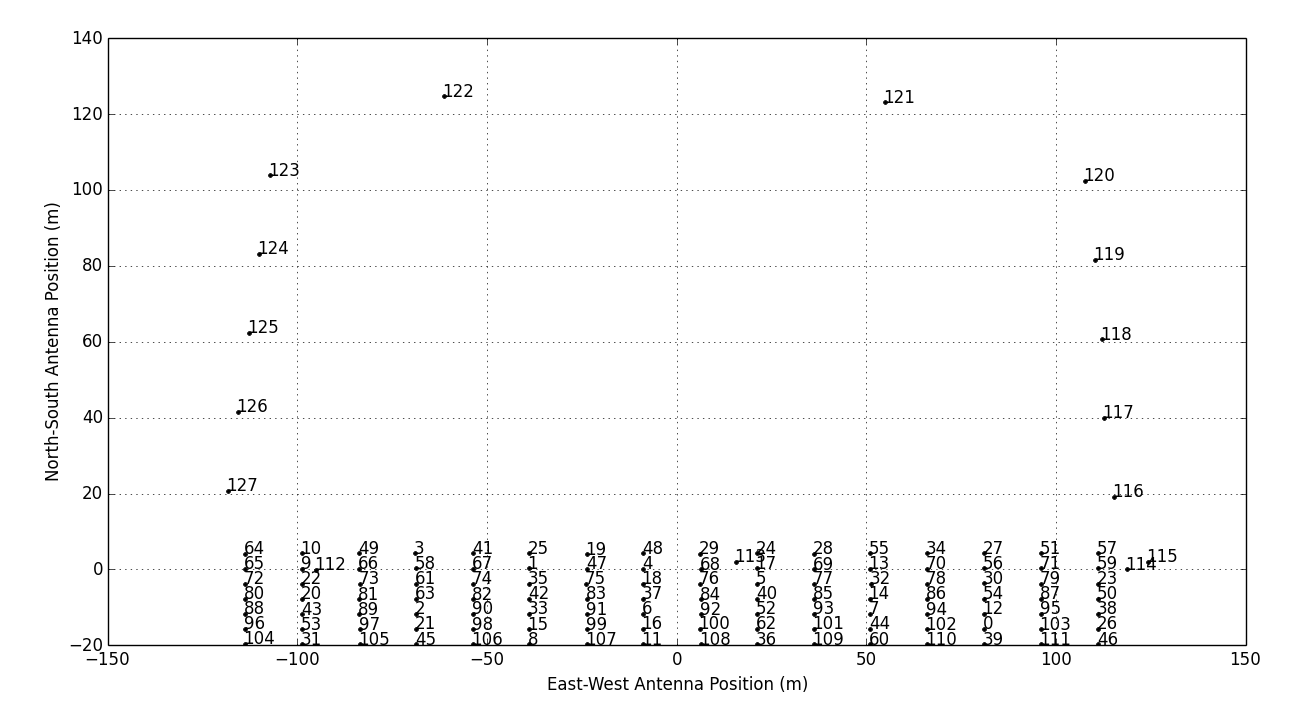
\includegraphics[width=0.96\textwidth]{plots/paper128_layout.png}
	\caption{The PAPER-128 antenna layout. There are 112 antennas arranged in a grid layout which are used for power spectrum analyses. The addition of 16 outrigger antennas is used to increase \textit{uv}-plane sampling for imaging analyses.}
	\label{fig:paper128_array}
\end{figure}

In general, the signal chain of PAPER-128 is similar to that of PAPER-64. However, one major change is the addition of receiverators on site, which houses the receivers used to amplify and filter the antenna signals. Prior to this change, the receivers were located inside a cooled shipping container along with the rest of the DSP system. With the addition of more antennas, however, the receivers were moved outside the container to save space. 

Although PAPER-128 doubled in number of antennas, the data collected by this array is typically found to be lower in quality than that of PAPER-64. There are many reasons for this, including general wear and tear on the instrument and the addition of the receiverators (which had no monitoring system and, as we will see, is one of the main reasons for missing and corrupted PAPER-128 data). Because of these issues, PAPER-128 requires the development of novel techniques in order to filter out contaminated data products prior to analysis. Using the entire season of data, without any filtering, would result in a power spectrum analysis severely dominated by systematics and (non-EoR) detections. Thus, one of the unique challenges facing PAPER-128 is how to automatically and accurately detect and remove bad data (i.e., misbehaving baselines, dead receiverators, criss-crossed signal paths, etc.) in order to curate a dataset as free of systematics as possible.

In this chapter, we present methods developed for the detection of corrupt data in PAPER-128. These methods represent the first routinely-used ``quality assurance" steps for the PAPER experiment. They also represent the first generation of data assessment techniques that are currently being expanded upon for incorporation into HERA's real-time processing system. 

\begin{table}[]
\begin{tabular}{|c|c|c|c|c|}
\hline
\textbf{Epoch} & \textbf{Dates}        & \textbf{\begin{tabular}[c]{@{}c@{}}Number of \\ Days Analyzed\end{tabular}} & \textbf{Flagged Days}                                                    & \textbf{Flagged Antennas}                                                                                                                         \\ \hline
1              & \begin{tabular}[c]{@{}c@{}} Nov 2013 - Jan 2014 \\ JDs 6617-6673\end{tabular}   & 38                                                                          & \begin{tabular}[c]{@{}c@{}}6647,6662,6664,\\ 6665,6673\end{tabular}      & \begin{tabular}[c]{@{}c@{}}3,7,8,16,19,20,\\ 27,28,34,53,\\ 56,84,85,96,100\\ \textbf{FX2}: 2,10,15,22,31,\\ 33,42,43,47,58,\\ 64,72,91,97,105,107\end{tabular} \\ \hline
2              & \begin{tabular}[c]{@{}c@{}} Jan 2014 - March 2014 \\JDs 6678-6724\end{tabular} & 40                                                                          & \begin{tabular}[c]{@{}c@{}}6692,6702,6704,\\ 6706,6717,6730\end{tabular} & \begin{tabular}[c]{@{}c@{}}3,7,16,27,34,56,\\57,84,85,100,110\end{tabular}                                                               \\ \hline
\end{tabular}
\caption{An overview of the PAPER-128 data used for power spectrum analysis in this thesis.}
\label{table:psa128_overview}
\end{table}

Additionally in this chapter, we process two epochs of PAPER-128 data (both from the first season) and show power spectrum results for each. We do not show results from the second season of data due to increased hardware failure that was experienced at the end of PAPER-128's deployment. As such, the first season of PAPER-128 represents the bulk of the array's sensitivity (though we note that the limits do not surpass those of PAPER-64, mostly due to having fewer days of data). Table \ref{table:psa128_overview} gives an overview of the PAPER-128 dataset analyzed in this thesis.

\section{Quality Assurance}

Post-processing of PAPER data relies heavily on the array's redundancy, and any sources of non-redundancy have the potential to corrupt redundant calibration and power spectrum estimation. These sources of error --- which span from the failure of analog or digital components to improper feed installation to the accidental deletion and subsequent recovery of data products --- manifest themselves in corrupted data that can be found primarily along two main axes: the time-axis and the antenna-axis. 

We next present metrics that we have developed to locate contaminated data along these axes. We use the results of these metrics to remove specific days of data and specific antennas from our analysis prior to calibration in order to ensure robust calibration that is not influenced by outlier data.

\subsection{Flagging Julian Dates}

To better assess the variation of PAPER-128 data across its two-year deployment (which consists of 7+ individual epochs of data, where an epoch is characterized by the shut-down and subsequent re-starting of the correlator), we first investigate one-dimensional slices of compressed data that span the entire time axis but only one frequency channel. We choose channel 100 for this analysis, as its corresponding frequency of 150\,MHz lies in the middle of our band (similar to PAPER-64, PAPER-128's bandwidth consists of 203 frequency channels ranging from 100 to 200\,MHz).

We look at the visibility amplitude of each day of data in an epoch as a function of LST, shown as the different colors in Figure \ref{fig:psa128_meanVij}. We designate a reference day to each epoch (a manually chosen ``good" day), and flag days that differ from the reference day by more than 20\%. After flagging, visibilities show good day-to-day agreement across an epoch (bottom row of Figure \ref{fig:psa128_meanVij}.

An example of data from a particularly ``bad" day is shown in Figure \ref{fig:psa128_badday}. It is clear that Julian date 2456692 differs dramatically from reference day 2456680, as it contains many corrupted files throughout the day due to failure somewhere in the signal chain. This failure mode is often due to the accidental deletion and erroneous recovery of data (much of the season's data was accidentally deleted prior to any of the work in this thesis), as well as hardware failures (e.g., loose cable connections) that result in lost sky fringes. From Table \ref{table:psa128_overview}, we see that a total of 38 days pass our flagging metric for Epoch 1 and 40 days pass for Epoch 2 (both from PAPER-128's first observing season), and a total of five and six days are flagged for each epoch, respectively.

\begin{figure*}
	\centering
	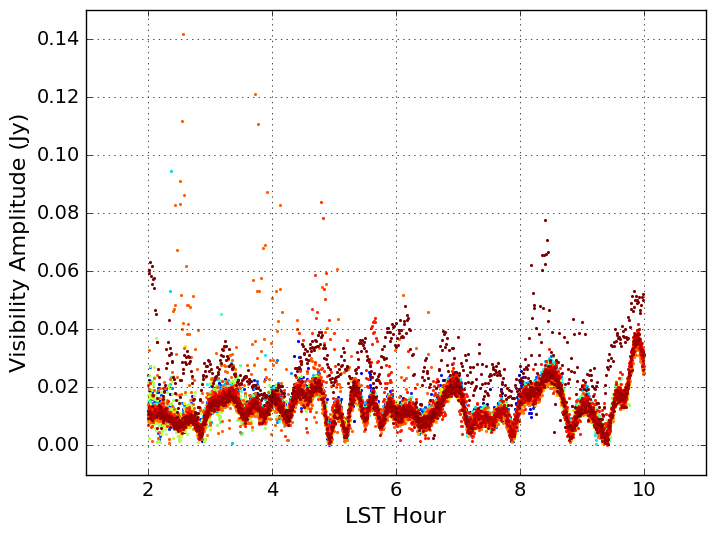
\includegraphics[trim={0cm 0cm 0cm 0cm},clip,height=0.35\textwidth]{plots/psa128_meanVij_S1E1_before.png}
	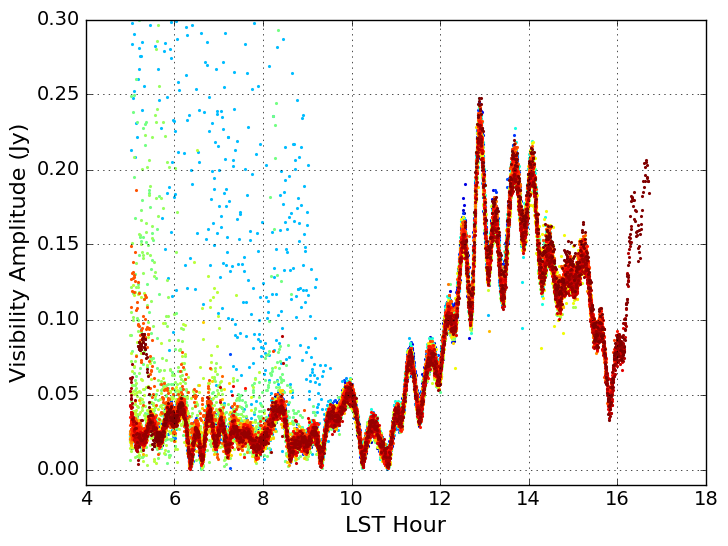
\includegraphics[trim={0cm 0cm 0cm 0cm},clip,height=0.35\textwidth]{plots/psa128_meanVij_S1E2_before.png}
	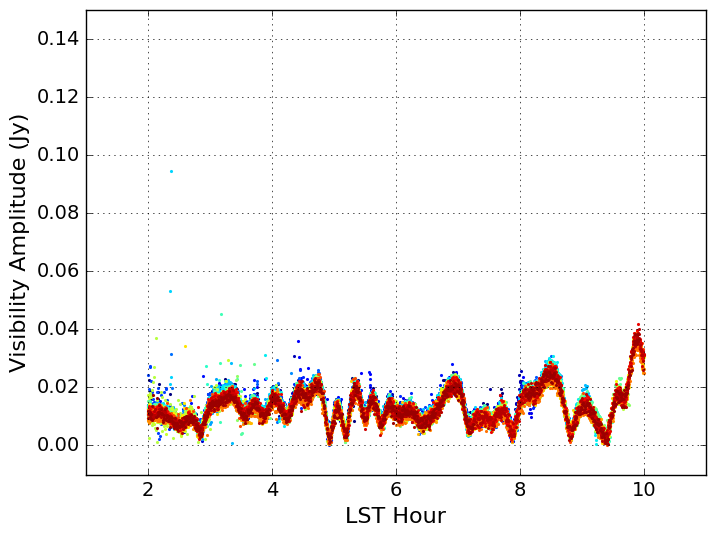
\includegraphics[trim={0cm 0cm 0cm 0cm},clip,height=0.35\textwidth]{plots/psa128_meanVij_S1E1_after.png}
	\includegraphics[trim={0cm 0cm 0cm 0cm},clip,height=0.35\textwidth]{plots/psa128_meanVij_S1E2_after.png}
	\caption{Visibility amplitudes as a function of LST for different Julian days of data (colors). The left column shows the data before (top) and after (bottom) the flagging of outlier days for Epoch 1. The right column shows similar data for Epoch 2. After flagging, visibilities show good day-to-day agreement across an epoch.}
	\label{fig:psa128_meanVij}
\end{figure*}

\begin{figure}
	\centering
	\includegraphics[width=0.8\textwidth]{plots/psa128_badday.png}
	\caption{Waterfall plots of visibility amplitudes for a ``good" reference day (left) in Epoch 2 and ``bad" day (right). We exclude corrupted data for specific days found with our metric.}
	\label{fig:psa128_badday}
\end{figure}

\subsection{Flagging Antennas}
\label{sec:psa128_badant}

There are a few types of failure modes for data associated with specific antennae. The first is if feeds are accidentally rotated by 90 degrees (or equivalently, the cables for the XX and YY polarizations are swapped). Consequently, visibilities involving a ``cross-polarized" antenna exhibit visibility amplitudes that are more weakly correlated (lower amplitude) than what is expected for an XX or YY visibility (and similarly, XY and YX visibilities exhibit too high of an amplitude, or too strong of a correlation). In order to locate potentially cross-polarized antennas, we use the following metric:

\begin{equation}
\label{eq:psa128_badant}
M_{i} = \frac{\sum\limits_{j,\nu,t} |V_{ij}|}{(N-1)},
\end{equation}
where the visibility for baseline $ij$ is summed for every $j^{th}$ antenna, frequency $\nu$, and time $t$, and $N$ is the number of antennas. We compute this metric for all four polarizations (XX, XY, YX, YY). Next, for each night of data we form the polarization fraction quantity:

\begin{equation}
\label{eq:psa128_crosspol}
P_{i} = \frac{M_{i}^{XY} + M_{i}^{YX}}{M_{i}^{XX} + M_{i}^{YY}}.
\end{equation}
We expect the numerator of this quantity to be higher than the denominator for cross-polarized antennae. In practice, we form polarization fractions for every antenna and flag those with high $P_{i}$ values as being cross-polarized. We note that this metric works best for long baselines, where XX and XY visibilities are expected to have large differences in signal-to-noise over short distance scales. For short baselines (and large-scales), astrophysical polarization has been shown to be present in all polarization quantities, including the linear ones, thus bringing $P_{i}$ closer to unity (\citealt{lenc_et_al2016}).

Using this metric, we find six antennas to be cross-polarized in PAPER-128 observations (antennas 26, 34, 38, 46, 50, and 72). An example of visibilities containing antenna 26 is shown in Figure \ref{fig:psa128_crosspol}, and it is clear that the ``X" and ``Y" polarizations are swapped for baselines involving that antenna. We fix this issue, re-naming polarization states where necessary, for all the compressed PAPER-128 data before performing other quality assessment tests and calibration.

\begin{figure}
	\centering
	\includegraphics[width=0.96\textwidth]{plots/psa128_crosspol.png}
	\caption{Waterfall plots of visibility amplitudes for four different polarizations and two different baselines. Antenna 26 is found to be cross-polarized because its feed was rotated by 90 degrees, and hence its ``X" and ``Y" polarization states are mis-labeled. Equation \eqref{eq:psa128_crosspol} captures visibility amplitudes like the ones shown here in order to automatically detect cross-polarized antennae.}
	\label{fig:psa128_crosspol}
\end{figure}

Another failure mode is an antenna that exhibits low amplitude, a fairly common occurrence as different electronic components can cause the temporary reduction or loss of power. A drastic example of this is when an entire correlator (FX2) was accidentally shut-off, cutting off connections to 16 antennas. The loss of those 16 antennas only affected Epoch 1, and the correlator was then re-started for Epoch 2. 

In order to find antennas with unusually low signals, we again employ Equation \eqref{eq:psa128_badant}, computing the metric for every antenna. Comparing $M_{i}$ across the entire array can reveal which antennas are consistently misbehaving. We then flag antennas with $M_{i}$ values that are low by at least $1\sigma$. Figure \ref{fig:psa128_badants} shows these antenna flags across both epochs, and we remove all data associated with antennas that are flagged greater than 50\% of the time (then for each epoch, we combine the flags for the XX and YY polarizations).

\begin{figure}
	\centering
	\includegraphics[trim={0cm 0cm 0cm 0cm},clip,height=0.35\textwidth]{plots/psa128_badants_S1E1.png}
	\includegraphics[trim={0cm 0cm 0cm 0cm},clip,height=0.35\textwidth]{plots/psa128_badants_S1E2.png}
	\caption{Flagged antennas, found using Equation \eqref{eq:psa128_badant}, are marked in black for each antenna number (x-axis) and Julian date (y-axis). The left column shows flags for XX polarization, and the right column shows flags for YY polarization. The top row shows flags for Epoch 1 and the bottom row shows flags for Epoch 2. We remove antennas that are flagged greater than 50\% of the time per epoch.}
	\label{fig:psa128_badants}
\end{figure}

Almost all of the flagged antennas listed in Table \ref{table:psa128_overview} are found via the metric described above. However, we do note that a handful are found manually by visually inspecting visibility data and {\tt Omnical} results. While our metric does a good job identifying antennas with low amplitudes, we found that there were certain antennas (usually one-off instances) with additional issues that do not fall under any of our previous metrics and would require a more sophisticated metric to be able to find automatically.

Finally, we highlight the importance of flagging antennas prior to redundant calibration by showing {\tt FirstCal} phase solutions for a single antenna without flagging and with flagging (Figure \ref{fig:psa128_chisq}, top). {\tt Omnical} $\chi^{2}$ results are also shown (bottom). These results depict how the quality of redundant calibration (the stability of the calibration solutions and level of redundancy) depends on the behavior of the antennas. It is evident that the {\tt FirstCal} solutions are unstable from file to file without any initial antenna flagging (top left). Similarly, higher $\chi^{2}$ values means that the {\tt Omnical} model visibilities differ substantially from the gain-corrected measured visibilities, meaning redundant calibration is poor. It is obvious that pre-calibration flagging metrics are crucial in order to robustly calibrate PAPER-128 data.

\begin{figure}
	\centering
	\includegraphics[trim={0cm 0cm 1cm 0cm},clip,height=0.35\textwidth]{plots/S1E1xx_nobadants_firstcal.pdf}
	\includegraphics[trim={0cm 0cm 1cm 0cm},clip,height=0.35\textwidth]{plots/S1E1xx_withbadants_firstcal.pdf}
	\includegraphics[trim={0cm 0cm 1cm 0cm},clip,height=0.35\textwidth]{plots/S1E1xx_nobadants_chisq.pdf}
	\includegraphics[trim={0cm 0cm 1cm 0cm},clip,height=0.35\textwidth]{plots/S1E1xx_withbadants_chisq.pdf}
	\caption{{\tt FirstCal} phase solutions for Antenna 1 (Epoch 1, XX polarization) where no antennas are flagged (top left) and some antennas are flagged (via the methods described in Chapter \ref{sec:psa128_badant}, top right). Omnical $\chi^{2}$ results are also shown for the two cases (bottom). We do not include any of the 16 dead antennas associated with correlator FX2. It is crucial to flag misbehaving antennas (especially extreme outlier antennas) prior to redundant calibration, motivating the development of automated quality assessment tools prior to the post-processing of data.}
	\label{fig:psa128_chisq}
\end{figure}

\section{Data Processing}

We process both epochs of PAPER-128 data, closely following the PAPER-64 processing steps outlined in Chapter \ref{sec:PSA64_processing}. One specific difference from the PAPER-64 pipeline is that we aggressively flag RFI prior to delay-filtering in order to prevent low levels of spectral structure from leaking into the EoR window. Because the overall quality of PAPER-128 data is in general lower than PAPER-64, we found that aggressive flagging methods are worthwhile in order to maximize signal-to-noise. To accomplish this, we first flag calibrated visibilities on a per-frequency, per-integration basis based on {\sc Omnical} $\chi^{2}$ values (using a $6\sigma$ deviation cutoff). This masks potentially problematic data identified from the redundant calibration solutions. In addition, we manually flag ten known channels containing RFI. 

Delay-filtering proceeds identically to the PAPER-64 pipeline. We then bin both the foreground-containing and foreground-removed data by LST into separate datasets. For both these datasets, we form Stokes I using Equation \eqref{eq:stokes}.

Recalling that redundant calibration only solves for internal calibration parameters, absolute calibration remains needed. In the PAPER-64 analysis, a self-calibration method was used to solve for overall gain and phase calibration solutions (immediately after redundant calibration) (\citealt{ali_et_al2015}). Trusting these solutions, we can then calibrate the PAPER-128 data to the calibrated PAPER-64 data. To do this, we use foreground-containing, LST-binned data for both PAPER-64 and PAPER-128 (where the PAPER-64 dataset is already calibrated) and look at a matching fiducial baseline for each. We align both datasets in LST and compute the ratio of the two for every time integration and frequency channel. We then average these ratios over time to yield a bandpass solution. 

Mathematically, if the visibility data for PAPER-64 and PAPER-128 are written as the following complex numbers:

\begin{eqnarray}
V_{64} = ae^{i\phi_{a}} \\
V_{128} = be^{i\phi_{b}},
\end{eqnarray}
we solve for an overall gain correction factor as:

\begin{equation}
f_{gain} = \frac{a}{b}
\end{equation}
and an overall phase factor as:

\begin{equation}
f_{\phi} = \phi_{a} - \phi_{b}.
\end{equation}
Combining these two gives a bandpass solution (one number per frequency):

\begin{equation}
f = f_{gain}e^{if_{\phi}}.
\end{equation}

Using this bandpass, we fit an eighth order polynomial to smooth the solutions and apply this multiplicative factor to the delay-filtered, LST-binned PAPER-64 data. We calibrate each epoch of data separately. We note that this coarse absolute calibration is only a rough calibration, and a more careful, sky-based calibration is recommended for precise results. However, using this simple calibration yields foreground data that agrees with the PAPER-64 data to within $\sim20\%$.

Finally, the last step of processing is fringe-rate filtering, where an optimal filter is used to combine the data and filter out excess noise. PAPER-128 has an original integration time of 32\,s, making the optimal filter length to be $\sim3910$\,s, slightly longer than that of PAPER-64. Armed with fringe-rate filtered, LST-binned datasets for both epochs, we proceed to power spectrum estimation.

\section{Power Spectrum Limits}

We form power spectrum estimates for both epochs of data and two frequency channel ranges: 139-149\,MHz (z=8.9) and 154-164\,MHz (z=7.9). Both bands consist of $21$ channels (each 0.5\,MHz) and are relatively absent of RFI. We focus only on one baseline-separation type, namely all 30\,m East/West baselines (of which there are 51 in the first epoch and 79 in the second). Our power spectrum formalism follows the analysis outlined in Chapter \ref{c.PSA64} and uses all updated methods regarding bootstrapping and noise sensitivity estimation. Because empirical inverse covariance weighting is shown to be extremely lossy for fringe-rate filtered PAPER data (Chapter \ref{sec:siglossmethod}) and regularization techniques do not significantly improve power spectrum sensitivity (Chapter \ref{sec:Weight}), we form unweighted limits ($\textbf{C} \equiv \textbf{I}$) in an effort to present straightforward, reliable results.

Figure \ref{fig:psa128_ps} shows the power spectrum results for PAPER-128. The two epochs are displayed as columns and the two redshifts as rows. Black and gray data points represent positive and negative power spectrum values, respectively (calculated as the average power spectrum value over all baseline pairs), and they have $2\sigma$ error bars that are calculated from bootstrapping over baselines. The solid green curve is our theoretical prediction of our sensitivity, computed analytically using Equation \eqref{eq:sense}. This sensitivity prediction is also plotted as gray shaded regions around the data points.

We note that our best limit is (126.4\,mK)$^{2}$ at $k = 0.29\,h$ Mpc$^{-1}$ and $z=7.9$ (from Epoch 2). This is a factor of XXX higher than our best limit from PAPER-64 (which uses three baselines instead of just one). These limits are understandably comparable given that the PAPER-128 analysis uses fewer days of data (by a factor of $\sim2$). While it's certainly possible that combining multiple epochs of data together (and using more baseline types) may yield better limits, we do not think this analysis is worthwhile as the second season of data is severely dominated by systematics. Instead, we look forward to exciting future results from HERA, knowing that many of the techniques developed for both PAPER-64 and PAPER-128 are being incorporated and improved upon.

\begin{figure}
	\centering
	\caption*{\hspace{0.6cm} Epoch 1 \hspace{5.6cm} Epoch 2}
	\includegraphics[trim={0cm 0cm 0cm 0.7cm},clip,height=0.5\textwidth]{plots/PSA128_S1E1_80_100.pdf}
	\includegraphics[trim={0cm 0cm 0cm 0.7cm},clip,height=0.5\textwidth]{plots/PSA128_S1E2_80_100.pdf}
	\includegraphics[trim={0cm 0cm 0cm 0.3cm},clip,height=0.5\textwidth]{plots/PSA128_S1E1_110_130.pdf}
	\includegraphics[trim={0cm 0cm 0cm 0.3cm},clip,height=0.5\textwidth]{plots/PSA128_S1E2_110_130.pdf}
	\caption*{\vspace{0.005cm}}
	\caption{Power spectrum results for PAPER-128 season 1 data for two redshifts (rows) and two epochs (columns), using one baseline separation-type only (30\,m East/West baselines). Black and gray points represent positive and negative power spectrum values, respectively, with $2\sigma$ error bars determined from bootstrapping. The $2\sigma$ theoretical noise sensitivity prediction is shown in green. Gray shaded regions correspond to theoretical errors on each data point.}
	\label{fig:psa128_ps}
\end{figure}

\chapter{HERA}
\label{c.HERA}






\defcitealias{ali_et_al2015}{A15}

\chapter{Conclusion}
\label{c.conclusion}

The work presented in this thesis can be summarized as the following:

\begin{itemize}
\item The original 21\,cm power spectrum results from the 64-element configuration of PAPER, presented in \citetalias{ali_et_al2015}, have been found to suffer from cosmological signal loss associated with the use of empirical covariances. Qualitative and quantitative investigations of the origin of this loss have shaped a deeper understanding of why signal loss arises, how to mitigate it, and how data analysis choices affect loss and power spectrum sensitivities. From this work emerges a new method to quantify signal loss which sets a standard across the field as a whole in terms of performing detailed calculations and assessments of loss.
\item Numerous other power spectrum analysis errors that affect both \citet{parsons_et_al2014} and \citetalias{ali_et_al2015} have been discovered and revised. These errors mostly concern error estimation techniques used by PAPER. While both the empirical and theoretical errors were under-estimated in the original analyses, updated methods are used to produce the power spectrum results throughout this work. At a broader level, this work has influenced the development of additional error estimation techniques for both PAPER and HERA analyses in a push for more robust tests and validation.
\item Using a simplified pipeline and incorporating all updated methods, PAPER-64 places new 21\,cm upper limits across a range of redshifts that are competitive with results from other experiments. Most notably, novel components of this analysis include investigations of PAPER's redundancy, comparisons with sky simulations, and analyses of jackknife tests.
\item The 128-element configuration of PAPER has been found to present unique challenges in terms of data quality. Algorithms have been developed in order to locate and remove contaminated data, which are now standard quality-check measures that have been incorporated into HERA's real-time processing system. However, because the quality of PAPER-128 data is poor compared to that of PAPER-64, we only present power spectrum results for two epochs of data, which are found to be comparable to the revised PAPER-64 results.
\item Initial HERA analyses are ongoing and signal loss characterization continues in an effort to build intuition behind our power spectrum analysis choices. Preliminary work suggests that the shape and accuracy of an eigenspectrum of a covariance is closely related to the amount of signal loss that is incurred when weighting data by the covariance. Future work in characterizing eigenspectra will help in understanding the interplay between convergences, weightings, and signal loss.
\end{itemize}

Taken as individual parts, the work in this thesis represents a collection of subtle lessons concerning 21\,cm power spectrum estimation. But looked at as a whole, it tells a bigger story that serves as a reminder of the uncertainty, challenges, and unpredictability of science in general. What began as a promising future for PAPER-128 (following a field-leading result from PAPER-64) led to the discovery of errors in PAPER-64 and subsequently an unanticipated retraction and revision. However, it is important to remember that good science --- regardless of the final outcome --- is science that is honest, careful, repeatable, and communicated. The broader story told in this thesis is, in some ways, one of unexpected failure. But it is also clear that the issues found are not unique to any one experiment and are pushing scientific progress in an untraditional way. As we close the chapter on PAPER, the lessons we have learned will continue to positively influence the path ahead, as unpredictable as it may be. What is predictable, though, is that we are now equipped with better tools and deeper understandings, and the field of 21\,cm cosmology has a lot to look forward to. 





\bibliography{thesis}{}

\end{document}
